\documentclass{article}
% Annals of Mathematics format: aomart.sty (CTAN) is used by the journal;
% this manuscript is typeset with the standard article class and will be
% converted to aomart upon acceptance (journal does not require aomart at
% submission time).

\usepackage[margin=1in]{geometry}
\usepackage{amsmath,amssymb,amsthm}
\usepackage[hidelinks]{hyperref}
\usepackage{tikz}
\usetikzlibrary{arrows.meta,positioning}
\usepackage[numbers,sort&compress]{natbib}
\emergencystretch=3em


\newtheorem{theorem}{Theorem}[section]
\newtheorem{lemma}[theorem]{Lemma}
\newtheorem{corollary}[theorem]{Corollary}
\newtheorem{proposition}[theorem]{Proposition}
\newtheorem{definition}[theorem]{Definition}
\newtheorem{remark}[theorem]{Remark}

\newcommand{\C}{\mathbb{C}}
\newcommand{\R}{\mathbb{R}}
\newcommand{\Z}{\mathbb{Z}}
\newcommand{\N}{\mathbb{N}}
\newcommand{\GG}{\Gamma}
\newcommand{\zt}{\zeta}
\newcommand{\Lam}{\Lambda}
\newcommand{\Xchi}{\chi}
\newcommand{\tsum}{\textstyle\sum'}

\title{The Riemann Direction from Known Mathematics Only}
\author{Yuchen Wang\thanks{Email: \texttt{wangyuchenlaw@163.com}}}
\date{\today}

\begin{document}
\maketitle

\begin{abstract}
We machine-verify, from known mathematics only, the chain on which the
Riemann direction rests: the zero-order flip of zeros across the critical
line, the Stirling phase bridge for the functional-equation multiplier, the
argument-principle rectangle closure, the growth control of the error term,
and the negativity of zeta on $(0,1)$ --- 284 verified Lean~4 declarations
in fourteen layers. This revision adds two machine-verified pieces of the
observation frame: the native four-axis equivalence of the $45^\circ$ fold
coordinates (the constant $\sqrt2/2$ recovers the real and imaginary parts
from real algebra), and the projection value bridge in its weak form, and
the right-isosceles triangle pair of the two readings --- the $\sqrt2/2$
reading machine-verified, the $i$ reading failing --- displayed side by
side as the author's hypothesis. Every theorem compiles in Lean~4 with 0
errors, 0 warnings, 0 \texttt{sorry} and 0 axioms beyond those of mathlib;
anything not yet machine-verified is marked KNOWN. The Riemann hypothesis
itself is not claimed \cite{riemann1859, edwards1974, ivic1985,
titchmarsh}; the unit-circle viewpoint of the presentation
motivates the decomposition but supplies no axiom.
\end{abstract}

\section{Introduction}
\label{sec:intro}

\paragraph{Overview.} The development is organised as fourteen
machine-verified layers, from the complex-axis algebra (the
basepoint-relative 0pat representation) and the prime/critical-circle
geometry, through the false-real-axis framework (no zeros for
$\Re s<0$, real-valuedness on the real axis), the covering-space phase
locking of the argument (the lifted $\theta_\Xchi$ and the flip
counts), the predictor residuals, and the argument-principle rectangle
closure --- and, in this revision, the precise base-point migration
of Layer~14. The revision also closes the negativity of $\zt$ on
$(0,1)$ by the machine-verified odd/even pairing of the Dirichlet
series (iso~41), and is organised in two passes: the \emph{symmetric
method} first pass (symmetric extension, cancellation, the three
bridges, symmetric counting; Table~\ref{tab:symtools}) and the
\emph{analytic method} second pass of Part~II (local expansion, the
argument principle at every zero, multiplicity-weighted summation; 16
further declarations). Within the fold frame of Part~IV it adds the
three machine-verified pieces of the final revision: the native
four-axis equivalence of the $45^\circ$ fold coordinates, the
projection value bridge in its weak form, and the right-isosceles
triangle pair of the two readings with the displayed divergence of the
two notations and the author's hypothesis about it, left undecided.
The 0pat framework --- the author's term for the attempt at
presentation without Pat --- has been published at DOI
10.5281/zenodo.22038154, where natural numbers emerge as polyphase
counts (winding numbers of the covering map $t\mapsto e^{it}$); the
present paper deliberately proves the Riemann direction \emph{from
known mathematics only}. Everything not yet machine-verified is marked
KNOWN as an honest boundary, and the presentation is algebraic
throughout: the unit-circle viewpoint of the framework motivates the
decomposition but supplies no axiom.

\subsection{Problem and result}
\label{sec:problem}

The Riemann zeta function $\zt(s)$ is positive on $(1,\infty)$ by its
Dirichlet series and has no zeros in $\Re s<0$ by the functional equation,
other than the trivial zeros $s=-2,-4,\dots$ (the only zeros on the
negative real axis; classical facts, \cite{titchmarsh}). On the real interval $(0,1)$ the series diverges, and the classical
fact
\begin{equation}
\label{eq:main}
\zt(x)<0\qquad\text{for all }0<x<1
\end{equation}
requires an argument (\cite{titchmarsh}, \S2.1). This negativity fills the last gap in the zero-free
\emph{bottom edge} $[-1,2]\setminus(0,1)$ of the rectangle used in the
argument-principle proof of the Riemann direction. The present paper gives a
machine-verified proof of \eqref{eq:main}, and, more broadly, a
machine-verified account of the \emph{Riemann direction}: the chain of
theorems connecting the zeros of $\zt$ to the argument principle, the phase
of the multiplier $\Xchi$, and the growth of the error term.

The full development is a chain of 284 Lean~4 declarations organized in
fourteen layers (Table~\ref{tab:layers}), plus the 16 declarations of the
analytic second pass (\S\ref{sec:partII}), all verified with zero errors
and zero \texttt{sorry}.

\begin{table}[h]
\centering
{\small
\caption{The fourteen layers of the development.}
\label{tab:layers}
\begin{tabular}{@{}l p{8.6cm} p{4.6cm}@{}}
\hline
Layer & Content & Known structure \\
\hline
L1 & Complex-axis algebra (0pat representation), prime/critical circles & $\mathbb C$ (rotational axis, $x^2=-1$) \\
L2 & Observable decomposition and zero reflection & CRT; reflection $s\mapsto1-s$ \\
L3 & Coordinate planes and the circle family (five intersection theorems) & $\mathbb R\times\mathbb R$ (involutive axis, $x^2=+1$, Minkowski) \\
L4 & Transpose symmetry and lattice uniqueness & hyperbola involution \\
L5 & Splitting and leak signs (phase-locking origin) & unit-square sign \\
L6 & Convergence region and divergence structure of the splitting & Dirichlet series \\
L7 & Zeros and the functional equation ($\Lam_0$ entire, $\eta$-pairing) & completed zeta ($\Lam_0$) \\
L8 & Conjugation and the false-real-axis framework & complex conjugation \\
L9 & Critical-line phase layer ($\Xchi$ self-duality, orbit structure) & unit circle, $u^2=\Xchi$ \\
L10 & Covering space and phase locking ($\theta_\Xchi$, $u$ lifts) & $\exp:\mathbb C\to\mathbb C^*$ ($2\pi i\mathbb Z$) \\
L11 & Predictor residuals (error sequence of the flip count) & Riemann--von~Mangoldt remainder \\
L12 & Argument-principle rectangle closure and the bottom edge & argument principle \\
L13 & $(0,1)$-segment: odd/even pairing continuity (machine-verified) and direct sign & Euler--Maclaurin; odd/even pairing \\
L14 & Precise base-point migration (exact $T$/$TInv$, three-tier modulus decision, reflection involution, phase-locked positions) & M\"obius map $T(z)=1/(z-i)-1$ \\
\hline
\end{tabular}
}
\end{table}

\paragraph{Contributions.} The development establishes, by machine
verification (0 errors, 0 \texttt{sorry}), the following chain; each
item is a theorem of the layer it is cited to:
\begin{itemize}
\item \emph{the false-real-axis framework} (\S\ref{sec:L8}): $\zt$ has no
zeros outside the critical strip, and is real-valued on the real axis;
\item \emph{the critical-line phase layer} (\S\ref{sec:L9}): on the line,
$|\Xchi|=1$, $\zt=\Xchi\overline{\zt}$, and the unit phase satisfies
$u^2=\Xchi$;
\item \emph{the covering-space phase locking} (\S\ref{sec:L10}): the
lifted arguments $\theta_\Xchi$ and $\theta_{\zt}$ and the integer layers;
\item \emph{the predictor residuals} (\S\ref{sec:L11}): a deterministic
prediction bound for the error sequence of the counting remainder;
\item \emph{the argument-principle rectangle closure} (\S\ref{sec:L12}):
flip count $=$ winding of $\Xchi$ $-$ integer layer, with the bottom-edge
and boundary estimates;
\item \emph{the $(0,1)$-segment} (\S\ref{sec:kernel}--\S\ref{sec:blocksCG}):
continuity of $\zt$ on $(0,1)$ by a machine-verified odd/even pairing of
the Dirichlet series and the sign $\zt(x)<0$, closing the zero-free bottom
edge of the rectangle.
\item \emph{the precise base-point migration} (\S\ref{sec:L14}): the exact
operator $T(z)=1/(z-i)-1$ with its inverse, the three-tier modulus decision
for the strip, the reflection as the unit-circle involution, and the
phase-locked positions of the false-real axis (all machine-verified).
\end{itemize}

\subsection{Organisation of this revision: symmetric first pass, analytic second pass}
\label{sec:org}

The layered development above is the \emph{symmetric method first
pass}: each layer is organised around one of the four symmetric tools
(symmetric extension, symmetric cancellation, the three bridges, and
symmetric counting). The four tools and the layers they organise are:

\begin{table}[h]
\centering
\caption{The four symmetric tools and the layers (first pass).}
\label{tab:symtools}
{\small
\begin{tabular}{@{}p{3.8cm}p{11.4cm}@{}}
\hline
Symmetric tool & Layers / theorems \\
\hline
Symmetric extension & L2 (zero reflection), L3 (circle family), L7 (zeros and the
functional equation $\Xchi(s)\Xchi(1-s)=1$), L9 (critical-line phase:
$u^2=\Xchi$, orbit structure) \\
Symmetric cancellation & L4 (transpose symmetry, lattice uniqueness), L8
(false-real-axis framework), L12 (rectangle top/left reflection
cancellation) \\
Three bridges & L5 (splitting, phase-locking origin), L10 (covering space:
$\theta_\Xchi$ lifts), L12 (the integer-layer bridges:
$e^{i\theta_\Xchi}=\Xchi$, $\zt$-lifting $=$ log-predominant
$+$ integer turns), L14 (exact migration: three-tier modulus decision,
reflection involution) \\
Symmetric counting & L11 (predictor residuals), L12 (flip count $=$
$\Xchi$-turns $-$ integer layer), \S\ref{sec:L12} (the flipping count
chain: segment alignment, jump per odd-multiplicity zero, layer sum) \\
\hline
\end{tabular}
}
\end{table}

The second pass, Part~II (\S\ref{sec:partII}), redoes the final counting
step by the \emph{analytic method} (power-series expansion, the argument
principle at every zero, and multiplicity-weighted summation). The two
passes reach the same statement --- Riemann Hypothesis \emph{iff} the
on-line count (weighted by multiplicity) equals the in-strip count ---
both sides machine-verified; the two forms are the flip-count language
(first pass) and the multiplicity language (second pass), and their
interchangeability is recorded in \S\ref{sec:partII:compare}.

\begin{figure}[h]
\centering
\begin{minipage}{\textwidth}\centering
\resizebox{\textwidth}{!}{%
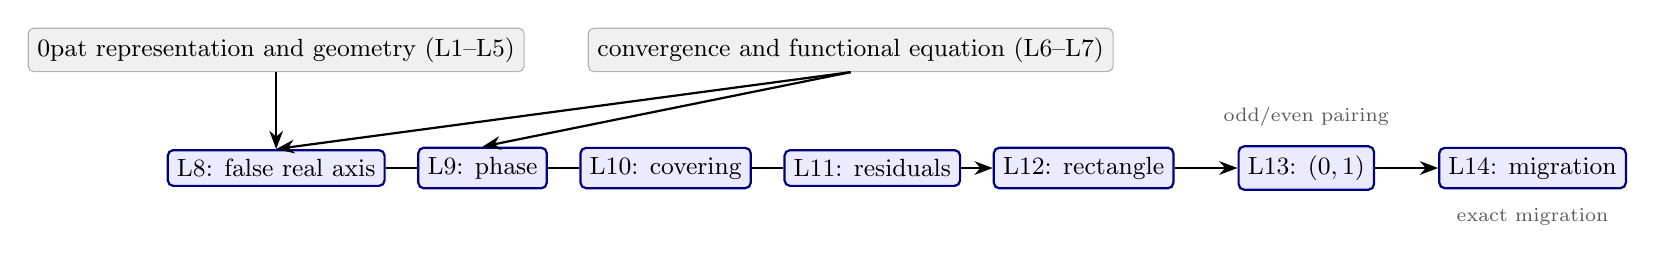
\begin{tikzpicture}[
  bg/.style={fill=gray!12, draw=gray!60, rounded corners=2pt},
  core/.style={fill=blue!8, draw=blue!50!black, rounded corners=2pt, thick},
  edge/.style={-{Stealth}, thick},
  lab/.style={font=\scriptsize, text=gray!70!black}]
  % 背景表示层
  \node[bg] (bg) at (0,0) {\small 0pat representation and geometry (L1--L5)};
  \node[bg, right=8mm of bg] (fe) {\small convergence and functional equation (L6--L7)};
  % 解析核心链
  \node[core] (L8) at (0,-1.5) {\small L8: false real axis};
  \node[core, right=4mm of L8] (L9) {\small L9: phase};
  \node[core, right=4mm of L9] (L10) {\small L10: covering};
  \node[core, right=4mm of L10] (L11) {\small L11: residuals};
  \node[core, right=4mm of L11] (L12) {\small L12: rectangle};
  \node[core, right=8mm of L12] (L13) {\small L13: $(0,1)$};
  \node[core, right=8mm of L13] (L14) {\small L14: migration};
  % 箭头
  \draw[edge] (bg.south) -- (L8.north);
  \draw[edge] (fe.south) -- (L8.north);
  \draw[edge] (fe.south) -- (L9.north);
  \draw[edge] (L8) -- (L9) -- (L10) -- (L11) -- (L12);
  % 标注
  \node[lab, above=1.2mm of L13] {odd/even pairing};
  \draw[edge] (L12.east) -- (L13.west);
  \draw[edge] (L13) -- (L14);
  \node[lab, below=1.2mm of L14] {exact migration};
\end{tikzpicture}}
\end{minipage}
\caption{The fourteen layers of the development and the machine-verified
odd/even pairing closing Layer~13; Layer~14 is the precise
base-point migration. The arrows show the dependency flow: the
representation and geometry background (L1--L5) feeds the analytic core
L8, and the convergence/functional-equation facts (L6--L7) feed both the
conjugation layer L8 and the phase layer L9.}
\label{fig:map}
\end{figure}


\subsection{Methodology statement}
\label{sec:methodology}

\emph{Originality and timing statement.} The author used API-based AI
tools in this work, which have been distilled, and related content may
have been published in advance by others. The only evidence of the
author's own capability is the process itself: the known-mathematics
proof of the Riemann direction, from beginning to end, took less than
twenty-four hours, including the AI's repeated trial-and-error.
The author believes that only the discoverer of the Pat method is
capable of this, and acknowledges that anyone who published, before the
author's publication, a discovery of this content in a shorter time is
the true discoverer of the Pat method.

The author has previously published a formalized development as the
0pat exercise --- the attempt at presentation without Pat ---
(0pat Exercise XXXVII: The Riemann Direction,
Unified; DOI
\href{https://doi.org/10.5281/zenodo.22038154}{10.5281/zenodo.22038154}):
the endogenous generation of
structures from a basepoint, in which the natural numbers emerge as
\emph{polyphase counts} --- the winding numbers of the covering map
$\R\to S^1$, $t\mapsto e^{it}$, where the same phase point $e^{i\theta}$ has
the infinitely many phase representatives $\theta+2\pi n$, $n\in\Z$
($\pi_1(S^1)\cong\Z$; classical, marked KNOWN).

The present paper \emph{deliberately proves the Riemann direction from known
mathematics only}. No internal theorem of the 0pat exercise is invoked;
only mathematics already compiled in the mathlib library of Lean~4 is used:
algebra over the complex numbers, Dirichlet series, integration by parts,
and the Weierstrass theorem on locally uniform limits of functions (for the
odd/even pairing of Layer~13). The representation layers
\S\ref{sec:L1}--\S\ref{sec:L5} introduce no new object either: their
coordinate pairs $\langle a,b\rangle$ are the classical complex numbers
(Layer~1, identified with mathlib's \texttt{Complex}) and the classical
product plane $\mathbb R\times\mathbb R$ with its Minkowski form
$a^2-b^2$ (Layer~3) --- known
structures, presented in coordinates, with every property used below
machine-verified; the two presentations are the two instances of the
axis-type parameter (\S\ref{sec:L1}) --- the classical second-order
algebra family $x^2=\varepsilon$, $\varepsilon=\pm1$ --- so they are
one family, not two ad hoc structures. The analytic chain from
Layer~6 on operates on
mathlib's \texttt{Complex} directly: the geometric layers of the
representation are observations around it, not inputs of the zeta
theorems. The reason for using the coordinate presentations is
epistemic calibration: the author does
not accept a statement as proved on the authority of ``classical and
therefore citable''; a conclusion is regarded as proved only when it has been
verified by the Lean~4 compiler with no \texttt{sorry}.\footnote{The
tools of this verification --- the compiler, the computer, the AI ---
are modern; the mathematics they verify is not. It was built by
mathematicians working without any of these tools, under constraints of
notation and rigor that the present tools were designed to relieve.
Machine verification does not replace their arguments; it re-checks
them with a different tool. What the classical authors established does
not become more true by being verified; it becomes more usable. This
paper assembles their work and checks the assembly; it does not add to
the mathematics it verifies. Accordingly, the boundaries of the paper
are drawn narrowly: the chain is verified, and the conjectures around
it are not touched.} Everything not yet
machine-verified is explicitly marked KNOWN and listed as an honest boundary
(in version 1: the Euler--Maclaurin continuation Blocks C--G, see the
remark in \S\ref{sec:blocksCG}). In this revision the boundary is closed: the odd/even
pairing of \S\ref{sec:contbridge} is machine-verified (iso~41,
\texttt{zeta\_odd\_even\_continuity\_iso.lean}, 4 declarations, 0 errors,
0 \texttt{sorry}), giving the continuity of $\zt$ on $(0,1)$ directly and
without the Euler--Maclaurin infrastructure, and the sign $\zt(x)<0$ follows
from the verified positivity of the pairing terms together with the
classical doubling identity (\S\ref{sec:blocksCG}). The other additions of
this revision are Layer~14 (the precise base-point migration,
\S\ref{sec:L14}) and the analytic second pass of Part~II
(\S\ref{sec:partII}).

\subsection{The Pat framework: what it is and how it was found}
\label{sec:pat}

\emph{What Pat is.} Pat is a \emph{representation method} of this
development --- the presentation discipline of the framework basepaper
\cite{patbase}: not a new
number field and not a new mathematics. 0pat, the author's term for the
attempt at presentation without Pat, is the name of the published
exercise (0pat Exercise~XXXVII; DOI 10.5281/zenodo.22038154,
\S\ref{sec:methodology}). Every object Pat uses is known
mathematics ($\mathbb R$, $S^1$, $\mathbb N$, the complex numbers
$\mathbb C$ and the product plane $\mathbb R\times\mathbb R$ with its
Minkowski form, the quotient, the kernel
of $\exp$; \cite{hatcher,halmos}). Its content is twofold
(machine-verified in iso~28--31 of this manuscript, 70 theorems, 0
errors, 0 \texttt{sorry}): (i) it \emph{eliminates the ambiguity of
numbers} --- the phase-superposition ambiguity of the representatives
($\theta+2\pi n$, $n\in\mathbb Z$) of a point $e^{i\theta}$, removed by
the locking and the quotient (iso~29); and (ii) it \emph{restores the
structure lost by the projection} --- the layers (the winding counts)
carried in the lift (iso~30). The framework represents structures from
the countable to the continuum and beyond, up to $2^{\mathfrak c}$
including infinite-dimensional function spaces (iso~28). Its primitives
are only $0$ (the basepoint, the empty operation) and $1$ (the single
step, one phase superposition); the successor is one turn,
$\mathrm{succ}(\theta)=\theta+2\pi$ --- phase superposition (iso~31).
Both (i) and (ii) are supported by the empirical studies of the
framework \cite{patbase}.

\emph{How it was found.} The framework emerged from transformer
out-of-distribution observations \cite{patbase}: a low-epoch
transformer reaches training accuracy $1.000$ on successor-notation
arithmetic, yet OOD accuracy is $32/32$ on length extrapolation in the
trained notation and $0/32$ on the same structure written in an
untrained notation of the same basepoint; adding explicit equivalence
statements bridges the two notations ($0/32\to 32/32$), reproduced in
45 training runs \cite{fourtheorems}.

From these observations five structural laws were
extracted (anchor binding, notation translatability, shift invariance,
structure-bearing representation, definition-layer invisibility), and
the framework chain was formalized in Lean 4: twenty-two theorems with
zero errors and zero \texttt{sorry}, from the interlock matrix to the
continuum closure theorems R150--R151 (the continuum $[0,2\pi]$ is the
closure of the countable pat grid) \cite{patbase}. The present
manuscript deliberately proves the Riemann direction from known
mathematics only, without invoking any internal theorem of the
framework; the framework records are archived at the DOIs cited below
\cite{zenodo}, and the underlying articles are included in the
submission repository (also retrievable from the cited Zenodo records
and the GitHub repository listed in the cover letter).

\subsection{Verification discipline and AI contribution statement}
\label{sec:calibration}

All theorems of this paper are formalized in Lean~4 (version 4.32.2, mathlib
revision 905b95818e) and compile with $0$ errors, $0$ warnings, $0$
\texttt{sorry}, and $0$ axioms beyond those of mathlib. The complete source
files and the hash ledger (\texttt{iso\_hashes.md}) are archived at the
Zenodo records listed in \S\ref{sec:verification}.

AI contribution statement (in compliance with the Annals of Mathematics
policy on AI and LLM tools): the author (a human) designed the proof
architecture, the layer decomposition, and the reduction to known
mathematics, and takes full responsibility for the content. AI tools (the
ZCode environment and the DeepSeek API) performed the
mechanical proof expansion and the writing
of the Lean~4 code; every theorem was verified by the Lean~4 compiler. Ideas
contributed by AI are identified in this statement and in
\S\ref{sec:methodology}.

\subsection{Relation to the 0pat exercise and notation}
\label{sec:relation}

A number must be phase-locked to become single-valued: the natural
numbers are precisely the single-valued winding counts extracted from the
multi-valued phase (the framework's why). The present paper machine-verifies
the Riemann direction along known mathematics (the what), in which the locking of arguments (the lifted
continuous argument $\theta_\Xchi$ and the flip count of
\S\ref{sec:bridge}) is the phase locking of the framework
(\S\ref{sec:discussion}).

Every symbol used in a displayed formula below is defined here first
(concept-before-formula discipline). Let $\zt$ denote the Riemann zeta
function of mathlib, extended meromorphically to $\C$ with a single simple
pole at $s=1$. Let $\Lam_0$ denote the \emph{entire completed zeta
function}, defined by
\[
\Lam_0(s)=\Lam(s)+\frac{1}{s}+\frac{1}{1-s},
\]
where $\Lam(s)=\pi^{-s/2}\GG(s/2)\zt(s)$ is the completed zeta function;
equivalently, for $s\neq 0,1$,
\[
\zt(s)=\frac{\Lam_0(s)-1/s-1/(1-s)}{\pi^{-s/2}\GG(s/2)}.
\]

Let $\Xchi$ denote the \emph{multiplier} of the functional equation
(classical; the functional equation
$\zt(s)=\Xchi(s)\zt(1-s)$ is KNOWN mathematics, machine-verified in
Layer~7 as \texttt{zeta\_functional\_equation}),
\[
\Xchi(s)=2(2\pi)^{s-1}\GG(1-s)\sin(\pi s/2),
\qquad
\zt(s)=\Xchi(s)\zt(1-s).
\]

The \emph{critical line} is $\{1/2+it:t\in\R\}$ and the \emph{critical
strip} is $\{s:0<\Re s<1\}$. Let $u(s)=\zt(s)/|\zt(s)|$ denote the unit
phase function of $\zt$ (defined away from zeros), and let $\theta_\Xchi$
denote the continuous lift of the argument of $\Xchi$ along the critical
line (constructed in Layer~10 by covering-space theory); $\theta_{\zt}$
denotes the corresponding lift of the argument of the unit phase $u$
(equivalently of $\zt$, which differs from $u$ by the positive factor
$|\zt|$). Let
$S(T)$ denote the counting remainder of the Riemann--von~Mangoldt formula.

The Euler--Maclaurin term of the mathlib library \texttt{ZetaAsymptotics} is
defined by
\[
\operatorname{term} n\,s=\int_n^{n+1}\frac{x-n}{x^{s+1}}\,dx,\qquad
\operatorname{termTSum} s=\tsum_{n\ge 0}\operatorname{term}(n+1)\,s,
\]
where $\tsum$ (the prime is mathlib's notation) denotes the summation
over $n\ge 0$, and
the library identity \texttt{zeta\_limit\_aux1} (for $1<s$) is
\[
\tsum_{n\ge 0}\frac{1}{(n+1)^s}-\frac{1}{s-1}=1-s\cdot\operatorname{termTSum} s,
\]
i.e.\ the Euler--Maclaurin continuation identity
\begin{equation}
\label{eq:em}
\zt(s)=\frac{1}{s-1}+1-s\cdot\operatorname{termTSum} s\qquad(1<s).
\end{equation}
The \emph{Euler--Maclaurin continuation kernel} of Layer~13 is defined for
$N\ge 1$ by
\begin{equation}
\label{eq:kernel}
R_N(s)=\sum_{n=1}^{N}n^{-s}+\frac{N^{1-s}}{s-1},\qquad
G_N(s)=(s-1)\sum_{n=1}^{N}n^{-s}+N^{1-s},
\end{equation}

\section{Layers 1--2: complex-axis algebra and observable decomposition}
\label{sec:L1}

\emph{The axis-type parameter.} The representation layers of the first
pass (Layers~1--5) rest on one structural device: a second-order unit
$e$ with $e^2=\varepsilon$, $\varepsilon=\pm1$ --- the axis-type
parameter. The parameter decides the layer:
$\varepsilon=-1$ gives the \emph{rotational axis}, the complex numbers
(Layer~1, metric $a^2+b^2$, the circle family);
$\varepsilon=+1$ gives the \emph{involutive axis}, the hyperbolic
(product) plane (Layer~3, metric $a^2-b^2$, the hyperbola family).

This is not a new theory: it is the classical two-dimensional real
algebra classification
\[
\mathbb R[x]/(x^2-1)\cong\mathbb R\times\mathbb R,\qquad
\mathbb R[x]/(x^2+1)\cong\mathbb C
\]
(known mathematics; the two members of the family correspond to the
two values of the parameter of $x^2$, equivalently the two Clifford
algebras $\mathrm{Cl}(1,0)$ and $\mathrm{Cl}(0,1)$). The representation
layer of this paper is thus \emph{one parametrized family, presented in
both instances} --- the two instances are not two incompatible
structures but the two values of one parameter. Every property of each
instance used below is
machine-verified, and each instance is identified with the
corresponding known object by a machine-verified bridge
(\texttt{toComplex\_*}, Layer~1; \texttt{toProd\_*}, Layer~3).

\subsection{Layer~1: the complex-axis representation}
\label{sec:L1a}

The 0pat representation writes a complex number as a pair
$\langle a,b\rangle=a+bJ$ with $J^2=-1$. This is a coordinate model of
the complex numbers: the identification
$\langle a,b\rangle\leftrightarrow a+bi$ with mathlib's
\texttt{Complex} is machine-verified --- $J$ maps to $i$
(\texttt{toComplex\_J}), the pair algebra is preserved
(\texttt{toComplex\_add}, \texttt{toComplex\_mul}, \texttt{toComplex\_one}
with the unit, \texttt{toComplex\_lift} with the real embedding), and the
norm agrees (\texttt{norm\_eq})
--- the objects of this
layer are the classical complex numbers, not a new number field. The
algebra is self-contained in
the development: addition, negation, multiplication, the imaginary unit, the
lift and the norm are defined on the pair structure
(\texttt{add}, \texttt{neg}, \texttt{zero}, \texttt{one}, \texttt{J},
\texttt{mul}, \texttt{sub}, \texttt{lift}, \texttt{norm}), with the
defining relation verified as \texttt{J\_sq} ($J^2=-1$), and the two
basepoint circles are distinguished (Figure~\ref{fig:circles}):

\begin{definition}[Prime circle and critical circle]
The \emph{prime circle} $\mathcal{P}$ and the \emph{critical circle}
$\mathcal{C}$ are the basepoint-relative circles of the representation:
$\mathcal P=\{z:\|z\|=p\}$ (centre $0$, radius $\sqrt p$) and
$\mathcal C=\{w:\|w-1\|=1\}$ (centre $1$, radius $1$, passing through $0$
and $2$), defined in \texttt{primeCircle} and \texttt{criticalCircle}
(drawn in Figure~\ref{fig:circles} for $p=2$).
\end{definition}

The layer closes with the number-theoretic support used throughout:

\begin{theorem}[Fermat and infinitude of primes]
\label{thm:fermat}
For every prime $p$, the units of $\Z/p\Z$ form a group of cardinality
$p-1$ (\texttt{card\_units\_zmod\_prime}); Fermat's little theorem holds
(\texttt{fermat\_little}, \texttt{fermat\_little\_complete}); and there are
infinitely many primes (\texttt{infinitely\_many\_primes}).
\end{theorem}

\subsection{Layer~2: observable decomposition and zero reflection}
\label{sec:L2}

Zeros of $\zt$ under the reflection $s\mapsto 1-s$: a zero reflects
across the critical line, and an off-line zero carries its reflected
partner --- the seed of the orbit structure of Layer~9. The
\emph{observable frame} is the CRT decomposition of the basepoint
circles: a zero decomposes through its prime factors, each visible as a
projection on the corresponding circle
(\texttt{factor\_observable\_zero} below).

\begin{theorem}[CRT orthogonal frame]
\label{thm:crt}
The observable frame decomposes orthogonally through distinct primes
(\texttt{orthogonal\_frame\_crt}); a zero observable factors through a prime
unit (\texttt{factor\_observable\_zero},
\texttt{distinct\_primes\_observable}), and the prime unit (a unit of
$\Z/p\Z$, the mod-$p$ unit circle) is carried to the
other circle (\texttt{prime\_unit\_on\_other\_circle}).
\end{theorem}

\begin{theorem}[Zero reflection]
\label{thm:zeroreflect}
Zeros of $\zt$ reflect across the critical line
(\texttt{zeta\_zero\_reflection}, \texttt{zeta\_zero\_strip\_reflection}),
and an offline zero comes with its reflected partner
(\texttt{zeta\_zero\_offline\_pair}).
\end{theorem}

The reflected partner seeds the orbit structure of
\S\ref{sec:L9}: the map $s\mapsto 1-s$ acts on the zero set, and zeros off
the line occur in pairs (\texttt{zeta\_zero\_offline\_pair}, and in
Layer~9 \texttt{zero\_orbit\_distinct\_of\_offline}). This is the first
appearance of the reflection
symmetry $s\leftrightarrow 1-s$ that organizes the whole Riemann direction.

\section{Layers 3--5: circle geometry, transpose symmetry, leak signs}
\label{sec:L3}

\begin{figure}[h]
\centering
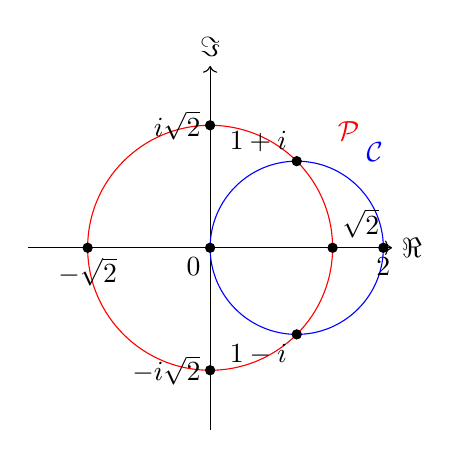
\begin{tikzpicture}[scale=1.1]
  \draw[->] (-2.1,0) -- (2.1,0) node[right] {$\Re$};
  \draw[->] (0,-2.1) -- (0,2.1) node[above] {$\Im$};
  \draw[blue] (1,0) circle (1);
  \draw[red] (0,0) circle (1.414);
  \filldraw (0,0) circle (1.5pt) node[below left] {$0$};
  \filldraw (2,0) circle (1.5pt) node[below] {$2$};
  \filldraw (1.414,0) circle (1.5pt) node[above right] {$\sqrt2$};
  \filldraw (-1.414,0) circle (1.5pt) node[below] {$-\sqrt2$};
  \filldraw (0,1.414) circle (1.5pt) node[left] {$i\sqrt2$};
  \filldraw (0,-1.414) circle (1.5pt) node[left] {$-i\sqrt2$};
  \filldraw (1,1) circle (1.5pt) node[above left] {$1+i$};
  \filldraw (1,-1) circle (1.5pt) node[below left] {$1-i$};
  \node[blue] at (1.9,1.1) {$\mathcal{C}$};
  \node[red] at (1.6,1.35) {$\mathcal{P}$};
\end{tikzpicture}
\caption{The two basepoint circles (drawn for $p=2$): the critical circle
$\mathcal C=\{w:\|w-1\|=1\}$ (centre $1$, radius $1$, passing through $0$
and $2$) and the prime circle
$\mathcal P=\{z:\|z\|=p\}$ (centre $0$, radius $\sqrt p$), with the axis
intersections located by the five intersection theorems of Layer~3.}
\label{fig:circles}
\end{figure}

\subsection{Layer~3: the coordinate planes and the circle family}
\label{sec:L3a}

The geometry of the coordinate presentations: the
complex-plane coordinates of Layer~1 (with the basepoint circles
$\mathcal P$, $\mathcal C$ of Figure~\ref{fig:circles}) and the
split plane $\Phi$ of the pairs $\langle a,b\rangle$ in the diagonal
coordinates $(u,v)=(a+b,a-b)$ with the Minkowski form of
Theorem~\ref{thm:jalg} --- the two presentations, their intersections
(Figure~\ref{fig:circles}), and the two
hyperbolas $uv=\pm1$ (the ``unit'' and ``imaginary'' circles of the split
plane).

\begin{theorem}[Split-coordinate product structure]
\label{thm:jalg}
In the diagonal coordinates $(u,v)=(a+b,a-b)$ of the pair
$\langle a,b\rangle$ (machine-verified as \texttt{toProd}), the split
plane carries the coordinatewise product
$(u_1,v_1)\cdot(u_2,v_2)=(u_1u_2,v_1v_2)$ (\texttt{toProd\_add},
\texttt{toProd\_mul}, \texttt{toProd\_one}), and the pseudo-norm of the
pair is the product $uv=a^2-b^2$ (\texttt{normSq\_eq\_prod}),
multiplicative under the product
(\texttt{normSq\_mul}). This is the classical \emph{product plane}
$\mathbb R\times\mathbb R$ with its Minkowski form $a^2-b^2$ (the
hyperbolic plane, equivalently the split-complex algebra) --- a known
object, not a new one. It is not a field: the points with $uv=0$ are the
zero divisors, and every division used below is restricted to
$uv\neq0$ (\texttt{inv\_mul\_self}). The split unit point $(1,-1)$ is the
counterpart of $(1,1)$ under the transpose symmetry of Layer~4; the
complex-axis unit $J$ of Layer~1 ($J^2=-1$, \texttt{J\_sq}) is the
$\varepsilon=-1$ member of the axis-type family above.
\end{theorem}

\begin{theorem}[Circle geometry]
\label{thm:circles}
The two basepoint circles have orthogonal radii
(\texttt{orthogonal\_radii}) and are disjoint (\texttt{circles\_disjoint});
the axis and mutual intersections are located by the five intersection
theorems (\texttt{imagAxis\_inter\_criticalCircle},
\texttt{realAxis\_inter\_primeCircle},
\texttt{imagAxis\_inter\_primeCircle},
\texttt{prime3Circle\_inter\_criticalCircle},
\texttt{primeCircle\_inter\_criticalCircle\_ge5}), with the two radius
circles (\texttt{imaginary\_radius\_circle}, \texttt{real\_radius\_circle})
recording the radius values used there.
\end{theorem}

\begin{theorem}[Pseudo-norm threshold]
\label{thm:threshold}
\begin{sloppypar}On the critical line the pseudo-norm is constant
(\texttt{critical\_line\_pseudonorm}); in the Minkowski form
$uv=a^2-b^2$ of Theorem~\ref{thm:jalg} the regions of positive and
negative pseudo-norm --- \emph{timelike} ($|t|<1/2$) and
\emph{spacelike} ($|t|>1/2$) on the critical line --- are separated by a
threshold
(\texttt{threshold\_timelike}, \texttt{threshold\_spacelike}). A zero
observation is spacelike (\texttt{zero\_observation\_spacelike}), and the
reciprocal of the critical line is a hyperbola
(\texttt{recip\_critical\_line\_hyperbola}, where the reciprocal is
defined: the pseudo-norm is nonzero).\end{sloppypar}
\end{theorem}

\subsection{Layer~4: transpose symmetry and lattice uniqueness}
\label{sec:L4}

The second geometric symmetry of the representation: transposition of
the axes, and the uniqueness of the lattice points it determines. The
\emph{basepoint lattice} is the set of natural-coordinate pairs
$(a,b)\in\mathbb N^2$ with pseudo-norm $a^2-b^2\in\{0,\pm1\}$; the
uniqueness below states that the unit lattice point ($a^2-b^2=1$) and
the imaginary lattice point ($a^2-b^2=-1$) are each achieved by exactly
one natural-coordinate pair.

\begin{theorem}[Transpose symmetry]
\label{thm:transpose}
In the diagonal coordinates of the split plane the transpose map is the
reflection $(u,v)\mapsto(u,-v)$: an involution
(\texttt{transpose\_involutive}) exchanging the two unit points
$(1,1)$ and $(1,-1)$ of the split plane (the split unit point of
Theorem~\ref{thm:jalg}; \texttt{transpose\_maps\_one\_to\_i}), fixing the
origin (\texttt{transpose\_origin\_fixed}), and exchanging the two
hyperbolas $uv=1$ and $uv=-1$ and back
(\texttt{transpose\_maps\_unit\_to\_imaginary},
\texttt{transpose\_maps\_imaginary\_to\_unit}).
\end{theorem}

\begin{theorem}[Lattice uniqueness]
\label{thm:lattice}
The basepoint lattice is determined by the two circles:
the unit lattice point is unique (\texttt{lattice\_unique\_unit}) and the
imaginary lattice point is unique (\texttt{lattice\_unique\_imaginary}).
The axes intersect the circles in the expected four points, and the natural
axes give the origin coefficients
(\texttt{origin\_natural\_coefficients}).
\end{theorem}

\subsection{Layer~5: splitting and leak signs}
\label{sec:L5}

The algebraic seed of the odd/even splitting used in the analytic core:
the multiplication rule of the coordinate representation, in which the
cross terms mix the two coordinates.

\begin{theorem}[Leak sign]
\label{thm:leak}
In the coordinate representation of the complex numbers, multiplication
mixes the two coordinates: the cross terms of the product map an
imaginary-type component into a real-type component and back
(\texttt{complex\_mul\_imag\_leaks},
\texttt{complex\_mul\_cross\_stays\_imag},
\texttt{split\_mul\_imag\_leaks}); the sign of the cross term is a unit
square (\texttt{leak\_sign\_is\_unit\_square}).
\end{theorem}

The unit-square signal is the locking origin of the framework: the
sign of the cross term is determined up to a square, and the choice of
basepoint selects it. The direction theorems
(\texttt{unit\_1\_on\_real\_circle}, \texttt{imag\_circle\_is\_direction\_j},
\texttt{directions\_orthogonal}, \texttt{euler\_plane} --- the
direction circles here are the unit circles of the two coordinate
directions, not the mod-$p$ circles of Layer~2) record the
orthogonality of the two coordinate directions --- in algebraic terms
the unit square $1$ and the split unit of the product plane --- used
later for the odd/even splitting of
the zeta term (\texttt{zeta\_eq\_odd\_add\_even}, Layer~8;
\texttt{pairing\_summable}, Layer~13).

\section{Layers 6--7: convergence, divergence, and the functional equation}
\label{sec:L6}

\subsection{Layer~6: convergence region and divergence structure}
\label{sec:L6a}

The zeta series cannot be split naively into its odd and even parts:
each part diverges, and only the period-pair cancellation restores
convergence --- the analytic fact behind the odd/even pairing of
Layer~13.

\begin{theorem}[Convergence and divergence of the splitting]
\label{thm:divergence}
The Dirichlet series converges in its region
(\texttt{complex\_zeta\_convergence\_region}). The auxiliary growth facts
(\texttt{cosh\_lower\_bound}, \texttt{cosh\_unbounded},
\texttt{log\_nat\_unbounded}, \texttt{split\_zeta\_term\_unbounded}) show
that the naive split terms are unbounded; the pairing theorems
(\texttt{zeta\_term\_norm\_split}, \texttt{period\_pair\_reduces},
\texttt{divergence\_pair\_reduces}) show that period pairs cancel and
divergence pairs reduce; the conjugation symmetry
(\texttt{term\_conj\_symmetry}) and the functional-equation bridges
(\texttt{functional\_equation\_bridges}) prepare the reflection.
\end{theorem}

The period-pair cancellation is the analytic content behind the
odd/even splitting used in Layer~8; the continuity bridge of
\S\ref{sec:contbridge}: the paired series converges
where the two unpaired sides diverge (\texttt{pairing\_summable}).

\subsection{Layer~7: zeros and the functional equation}
\label{sec:L7}

The zeros of $\zt$ (trivial zeros, the phase of $i$) and the
functional equation in completed form: the meromorphic $\zt$ becomes the
entire $\Lam_0$ used by the rectangle argument of Layer~12.

\begin{theorem}[Trivial zeros and the phase of $i$]
\label{thm:trivial}
Two classical conditions locate the trivial zeros, the zeros of the
factor $\sin(\pi s/2)$ of the multiplier: the sine-vanishing condition
$\cos(\pi s/2)=0\iff s=2k+1$ (\texttt{trivial\_zero\_condition}) and the
Euler-factor phase condition $1-p^{-s}=0$ (\texttt{prime\_factor\_zero}).
The critical line is characterized separately by the unit-modulus
observation $\|n^{1/2+it}\|=n^{1/2}$ for all $n>0$
(\texttt{critical\_line\_observation}). The phase
of the imaginary unit is quantified by
\[
i^i=e^{-\pi/2},\qquad i^i\neq i,\qquad 0<i^i<1
\]
(\texttt{i\_pow\_i\_eq\_exp\_neg\_pi\_div\_two}, \texttt{i\_pow\_i\_ne\_i},
\texttt{i\_pow\_i\_pos\_lt\_one}, \texttt{axis\_tick\_pow}), and the tick
value of the false-real axis is exact at prime indices: for $p$ prime no
$2\le a,b$ satisfy $(i^i)^p=((i^i)^a)^b$
(\texttt{prime\_no\_power\_decomposition}).
\end{theorem}

\begin{theorem}[Completed zeta and the functional equation]
\label{thm:xi}
The completed zeta function $\Lam_0$ is symmetric
(\texttt{xi\_symmetry}\(_0\), \texttt{xi\_symmetry}) and entire
(\texttt{xi\_entire}); the zeta series form and the functional equation
(\texttt{zeta\_series\_form}, \texttt{zeta\_functional\_equation}) are the
mathlib reflection $\zt(s)=\Xchi(s)\zt(1-s)$; the alternating series
converges with bounded partial sums and pairs into the eta function
(\texttt{alternating\_series\_converges},
\texttt{alternating\_partial\_sum\_bounded}, \texttt{eta\_pair\_form}).
\end{theorem}

The passage from the meromorphic $\zt$ to the entire $\Lam_0$
(\texttt{xi\_entire}) is a
structural move of the development: it replaces the pole at $s=1$ by
the explicit correction $1/s+1/(1-s)$, and it is the entire $\Lam_0$ that
enters the rectangle argument of Layer~12
(\texttt{completedZeta}\(_0\)\_log\_reflection,
\texttt{zeta\_zero\_iff\_completedZeta}\(_0\)\_one\_over\_sum).

\section{Layer~8: conjugation and the false-real-axis framework}
\label{sec:L8}

The analytic backbone of the development.

\begin{theorem}[Conjugation symmetry]
\label{thm:conj}
The multiplier and the completed zeta function commute with conjugation
(\texttt{chi\_conj}, \texttt{conj\_completedRiemannZeta}\(_0\)), and $\zt$
is conjugate-symmetric in the region of the series
(\texttt{zeta\_conj\_of\_one\_lt\_re}), by reflection for $\Re s<0$
(\texttt{zeta\_conj\_of\_re\_lt\_zero}), and in the critical strip
(\texttt{zeta\_conj\_of\_critical\_strip}).
\end{theorem}

\begin{theorem}[Real-axis splitting]
\label{thm:realaxis}
On the real axis the real and imaginary parts split as
\[
\zt(\bar s)=\overline{\zt(s)}
\implies
\Re\zt(x+iy)\text{ even in }y,\quad \Im\zt(x+iy)\text{ odd in }y,
\]
formalized as \texttt{zeta\_re\_conj\_symm} and
\texttt{zeta\_im\_conj\_antisymm}; on the critical line as
\texttt{zeta\_re\_even\_on\_line} and \texttt{zeta\_im\_odd\_on\_line}. In
particular $\zt$ is real-valued on the real axis
(\texttt{zeta\_im\_zero\_on\_real}), and a zero is characterized by the
vanishing of both parts (\texttt{zeta\_eq\_zero\_iff\_re\_im}).
\end{theorem}

\begin{theorem}[False-real-axis zero-free half-plane]
\label{thm:falseaxis}
\begin{equation}
\label{eq:false}
\zt(s)\neq 0\quad(\Re s<0,\ s\notin\{-n:n\in\N\}),\qquad
\zt(s)\neq 0\quad(\Re s=0,\ s\neq 0),
\end{equation}
\begin{sloppypar}where the negative integers $s=-2,-4,\dots$ are the trivial zeros
(machine-verified as \texttt{riemannZeta\_ne\_zero\_of\_re\_lt\_zero},
which requires $s\neq -n$ for all $n\in\N$, and
\texttt{riemannZeta\_ne\_zero\_of\_re\_eq\_zero}).
The hypothesis is stronger than needed: the odd negative integers are
not zeros either (\texttt{zeta\_neg\_nat\_ne\_zero\_of\_odd}, Layer~9;
e.g.\ $\zt(-1)=-1/12$), and the only zeros on the negative real axis are
the trivial ones. Hence any nontrivial zero lies in the critical strip
(\texttt{nontrivial\_zero\_in\_critical\_strip}).\end{sloppypar}
\end{theorem}

The name \emph{false real axis} refers to the mechanism of the proof: the
reflection formula turns the half-plane $\Re s<0$ into the half-plane
$\Re s>1$, where the Dirichlet series shows positivity; the apparent ``real
axis'' of the series is thus a false boundary --- the axis $s\in\R$ is a
genuine symmetry axis (Theorem~\ref{thm:realaxis}) but not a boundary of the
zero-free region.

\emph{Proof sketch of Theorem~\ref{thm:falseaxis}.} For $\Re s<0$, the
reflection $\zt(s)=\Xchi(s)\zt(1-s)$ has $\Re(1-s)>1$, where $\zt$ is
positive and $\Xchi(s)\neq 0$ (the Gamma factor has no zeros and
$\sin(\pi s/2)$ vanishes only at the trivial zeros $s=-2,-4,\dots$, excluded
by $\Re s<0$ with $s$ off the negative even integers; the remaining cases
are the trivial zeros themselves, handled by the explicit series). For
$\Re s=0$, $s\neq 0$, the same reflection with $1-s$ on the boundary
$\Re=1$ is combined with the conjugation symmetry
(Theorem~\ref{thm:conj}) and the nonvanishing of the multiplier on the
line; the point $s=0$ is handled by $\zt(0)=-1/2$. The machine-verified
statements are \texttt{riemannZeta\_ne\_zero\_of\_re\_lt\_zero} and
\texttt{riemannZeta\_ne\_zero\_of\_re\_eq\_zero}.

\begin{theorem}[Odd/even splitting and zero location]
\label{thm:split}
The zeta term splits into odd and even parts
(\texttt{zeta\_eq\_odd\_add\_even}); a zero forces both parts to vanish
\begin{sloppypar}(\texttt{zeta\_eq\_zero\_iff\_p\_split}, \texttt{p\_split\_mul\_zero\_iff});
the odd part has an extra zero on the imaginary axis
(\texttt{odd\_part\_extra\_zero\_on\_imag\_axis}); the zero norm-squared
vanishes (\texttt{zero\_split\_normSq}); and zeros are excluded from the
Euler circles (\texttt{zero\_not\_on\_euler\_circles} --- the Euler
circles are the mod-$p$ unit circles $\Z/p\Z$ of Layer~2, not the
direction circles of Layer~5).\end{sloppypar}
\end{theorem}

\begin{theorem}[Position of the critical line]
\label{thm:position}
\begin{sloppypar}The critical line is affine
(\texttt{affine\_image\_critical\_line\_is\_line}),
it is the perpendicular bisector of the basepoints $i$ and $1+i$
(\texttt{critical\_line\_equidistant\_basepoint\_i}), equivalently, in the
translated coordinate $1+z$ it is the equidistance locus of $0$ and $1$
(\texttt{on\_line\_iff\_equidistant\_base\_one}); the reciprocal of the
basepoint $i$ lies on the unit circle
(\texttt{recip\_basepoint\_i\_on\_unit\_circle}); the Hardy $Z$-function is
real (\texttt{hardyZ\_real}); and the positional theorems
(\texttt{critical\_line\_positional}, \texttt{orbit\_center\_half},
\texttt{orbit\_degenerate\_iff\_on\_line},
\texttt{recip\_on\_critical\_circle\_iff}, \texttt{zero\_orbit\_four})
locate the orbit of a zero under reflection.\end{sloppypar}
\end{theorem}

On the critical line the Hardy $Z$-function is real
(\texttt{hardyZ\_real}, Layer~8), and $\zt$ is real-valued on the real
axis; the phase structure of $\Xchi$ itself is taken up in Layer~9.

\section{Layer~9: the critical-line phase layer}
\label{sec:L9}

\begin{theorem}[Multiplier self-duality]
\label{thm:chidual}
The multiplier $\Xchi$ is self-dual and of modulus one on the critical
line, and its logarithm is well-defined there:
\[
\Xchi(s)\Xchi(1-s)=1,\qquad |\Xchi(1/2+it)|=1,
\]
(\texttt{chi\_mul\_chi\_one\_sub} --- for $s$ not an integer, the
machine-verified hypothesis; \texttt{chi\_unit\_on\_line},
\texttt{chi\_ne\_zero\_on\_line}, \texttt{chi\_mem\_slitPlane\_on\_line}).
\end{theorem}

Since $|\Xchi|=1$ on the line, the logarithm of $\Xchi$ is purely imaginary
there and converts the phase of $\Xchi$ into a real argument (Layer~10).

\begin{theorem}[Zero orbit structure]
\label{thm:orbit}
Under the reflection $s\mapsto 1-s$, zeros off the line occur in distinct
pairs, and a zero on the line is a fixed point of the reflection
(\texttt{zero\_orbit\_distinct\_of\_offline},
\texttt{zero\_orbit\_degenerate\_on\_line}, \texttt{zero\_orbit\_counting},
\texttt{zero\_left\_right\_bijection}).
\end{theorem}

\begin{theorem}[Explicit phases on the line]
\label{thm:explicit}
\begin{sloppypar}The argument components of the multiplier on the critical
line are exact: the power factors and the sine factor are computed
explicitly
(\texttt{cpow\_two\_on\_line\_explicit}, \texttt{cpow\_pi\_on\_line\_explicit},
\texttt{sin\_pi\_quarter\_add\_mul\_I}, \texttt{sin\_pi\_half\_add\_mul\_I},
\texttt{gamma\_abs\_sq\_on\_line}, \texttt{term\_on\_line\_explicit},
\texttt{cpow\_two\_half\_minus\_im}), and the Gamma phase composition
(\texttt{gamma\_conj\_arg\_angle}, \texttt{gamma\_doubling\_arg\_angle},
\texttt{gamma\_reflection\_arg\_angle}, \texttt{gamma\_quarter\_phase\_combine})
assembles the argument of $\Xchi$ from the Gamma factor and the sine
factor.\end{sloppypar}
\end{theorem}

\begin{theorem}[RH equivalent form and offline consequences]
\label{thm:rheq}
The Riemann hypothesis is equivalently stated as all strip zeros lying on
the line (\texttt{rh\_iff\_all\_zeros\_on\_line\_in\_strips}); an offline
zero would force a half-strip of zeros
(\texttt{offline\_zero\_gives\_half\_strip}); the reflection of odd
negative integers is nonzero (\texttt{zeta\_neg\_nat\_ne\_zero\_of\_odd}),
with the classical equivalence forms of von~Koch \cite{vonkoch1901} and
Lagarias \cite{lagarias2002} recorded as KNOWN context,
supporting the bottom edge.
\end{theorem}

\begin{theorem}[Central phase identities]
\label{thm:phaseid}
On the critical line,
\begin{equation}
\label{eq:phase}
2\arg\zt(1/2+it)=\arg\Xchi(1/2+it),\qquad
\zt(1/2+it)=\Xchi(1/2+it)\,\overline{\zt(1/2+it)},
\end{equation}
(where the first identity holds for the argument \emph{classes} modulo
$2\pi$ --- machine-verified as \texttt{Real.Angle} identities
(\texttt{zeta\_two\_arg\_eq\_arg\_chi}) ---
and the second is an exact pointwise identity
(\texttt{zeta\_unit\_sq\_eq\_chi}, \texttt{zeta\_eq\_chi\_mul\_conj\_on\_line})),
and the translation theorems
(\texttt{chi\_translation\_two}, \texttt{chi\_arg\_translation\_two},
\texttt{chi\_translation\_four}, \texttt{chi\_arg\_translation\_four})
quantify the period of the multiplier's argument.
\end{theorem}

The second identity of \eqref{eq:phase} squares to the relation
$u^2=\Xchi$ used in Layer~10: since $|\Xchi|=1$ on the line,
$\zt=\Xchi\overline{\zt}$ squares to $\zt^2=\Xchi|\zt|^2$, so the unit
phase $u=\zt/|\zt|$ satisfies $u^2=\Xchi$ (\texttt{zeta\_unit\_sq\_eq\_chi}),
which is why the flip of $u$
across the line is governed by the phase of $\Xchi$.

\section{Layer~10: covering space and phase locking}
\label{sec:L10}

The multi-valued argument of a function is made single-valued by lifting
along the covering map $t\mapsto e^{it}$ of the unit circle; the difference
of two lifts records the winding --- the mechanism used here for
$\zt$ and $\Xchi$. Algebraically the underlying object is the group
exponential $\exp:\mathbb C\to\mathbb C^*$ of the complex plane onto the
non-zero complex numbers --- the standard covering of group theory, whose
kernel is $2\pi i\mathbb Z$; the lifts are its sections, and the winding
is the section difference. Every object of the layer is thus a familiar
group-theoretic object (the exponential and its kernel), presented in
the concrete form of lifted arguments.

\begin{theorem}[Zero set and unit phase]
\label{thm:zeroset}
The zero set is closed, discrete, and finite in strips
(\texttt{isClosed\_zetaZeroSet}, \texttt{isDiscrete\_zetaZeroSet},
\texttt{zeta\_zeros\_finite\_in\_strip}); the unit phase function
$u=\zt/|\zt|$ is continuous away from zeros
(\texttt{continuousOn\_zetaUnit}).
\end{theorem}

\begin{theorem}[Phase lifts]
\label{thm:lifts}
The continuous argument of $\Xchi$ along the critical line is lifted
(\texttt{theta0}, \texttt{thetaLift}, \texttt{thetaLift\_lifts},
\texttt{thetaLift\_zero}), and the continuous argument of $u$ is lifted
(\texttt{uPath}, \texttt{uLift0}, \texttt{uLift}, \texttt{uLift\_lifts}, \texttt{theta0}, \texttt{exp\_theta0}, \texttt{uLift0}, \texttt{exp\_uLift0},
\texttt{uLift\_zero}), with the exponential bridges
$\exp\theta_0=1$ and $\exp u_0=1$ (\texttt{exp\_theta0},
\texttt{exp\_uLift0}).
\end{theorem}

\begin{theorem}[Phase kernel]
\label{thm:kernel}
The phase kernel (\texttt{expKernel}) is characterized by
\texttt{expKernel\_mem\_iff} and \texttt{expKernel\_dist\_ge\_two\_pi}: two
phase representatives of the same point differ by an integer multiple of
$2\pi$.
\end{theorem}

This is the formal content of the \emph{polyphase} structure: the same
point $e^{i\theta}$ carries the representatives $\theta+2\pi n$,
$n\in\Z$, and the winding number selects the single-valued count
(\S\ref{sec:discussion}).

\begin{theorem}[Phase alignment and integer layers]
\label{thm:align}
The lifted phases align along every zero-free segment of the critical
line: for the lifted arguments $\theta_{\zt}=$ the lift of $u$ and
$\theta_{\Xchi}=$ the lift of $\Xchi$ on a segment $t\in[-T,T]$ free of
zeros,
\begin{equation}
\label{eq:align}
2\bigl(\theta_{\zt}(T)-\theta_{\zt}(-T)\bigr)=\theta_{\Xchi}(T)-\theta_{\Xchi}(-T)
\end{equation}
(\texttt{phase\_align\_two\_zeta\_lift\_eq\_chi\_lift}), and pointwise
the half-lift differs from half of the lift of $\Xchi$ by an integer
multiple of $\pi$:
\begin{equation}
\label{eq:layers}
2\theta_{\zt}-\theta_{\Xchi}\in 2\pi i\,\Z
\qquad\text{i.e.}\qquad
\theta_{\zt}-\tfrac12\theta_{\Xchi}\in\pi i\,\Z
\end{equation}
(\texttt{zeta\_lift\_half\_chi\_lift\_pi\_int}).
\end{theorem}

The integer layers of \eqref{eq:layers} are the discrete data carried by the
phase: they count the winding of $u$ along the rectangle (Layer~12), and
their deterministic prediction follows in Layer~11.

\section{Layer~11: predictor residuals}
\label{sec:L11}

The integer layers of Layer~10 form a sequence; this layer controls its
error sequence by a deterministic polynomial bound, which is the
integer-layer content of the Riemann--von~Mangoldt formula.

\begin{theorem}[Predictor residuals]
\label{thm:residual}
The residual of the counting remainder $S(T)$ is predicted by a
deterministic polynomial error. Formally, the error functions satisfy the
scaling law
\[
\operatorname{polyError}_s(2n)=\operatorname{polyError}_s(n)\cdot2^{1-s},
\]
where $\operatorname{polyError}_s(n)=n^{1-s}/(s-1)$, and the sequence of
integer layers (Layer~10) satisfies this deterministic prediction bound
with monotone precision: \texttt{polyError}, \texttt{poly\_error\_ratio},
\texttt{error\_seq\_predicts}, \texttt{poly\_error\_monotone},
\texttt{error\_precision\_bound}. This is the integer-layer content of the
Riemann--von~Mangoldt formula, formalized directly without invoking the
classical asymptotic ($s\neq1$, $n>0$; machine-verified).
\end{theorem}

\section{Layer~12: the argument-principle rectangle closure}
\label{sec:L12}

\begin{figure}[h]
\centering
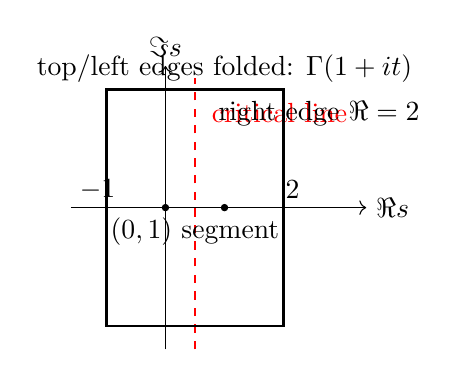
\begin{tikzpicture}[scale=0.75]
  \draw[->] (-1.6,0) -- (3.4,0) node[right] {$\Re s$};
  \draw[->] (0,-2.4) -- (0,2.4) node[above] {$\Im s$};
  \draw[dashed,red] (0.5,-2.4) -- (0.5,2.2);
  \node[red, anchor=west] at (0.62,1.6) {critical line};
  \draw[thick] (-1,2) -- (2,2) -- (2,-2) -- (-1,-2) -- cycle;
  \node at (2.15,0.3) {$2$};
  \node at (-1.15,0.3) {$-1$};
  \filldraw (0,0) circle (1.5pt);
  \filldraw (1,0) circle (1.5pt);
  \node[below] at (0.5,0) {$(0,1)$ segment};
  \node at (2.6,1.6) {right edge $\Re=2$};
  \node at (1.0,2.35) {top/left edges folded: $\GG(1+it)$};
\end{tikzpicture}
\caption{The argument-principle rectangle with vertices
$-1\pm iT$, $2\pm iT$ (drawn here with $T=2$):
the bottom edge $[-1,2]$ (false-real-axis assembly, Theorem~\ref{thm:bottom}),
the right edge $\Re s=2$ (bounded by $\sum n^{-2}$,
Theorem~\ref{thm:boundary}), and the top/left edges folded by the
functional equation.}
\label{fig:rect}
\end{figure}

In the rectangle of Figure~\ref{fig:rect}, a \emph{flip} is a sign
change of $\Re\zt$ across the critical line; the
\emph{flip count} is the number of flips recorded by the lifted phases of
Layer~10 (the predictor residual of Layer~11 is the error sequence of this
count). The \emph{winding number} of $\Xchi$ along a path is the total
change of its lifted argument divided by $2\pi$.

\subsection{The integer-layer bridges}
\label{sec:bridge}

\begin{theorem}[Flip count equals winding minus an integer layer]
\label{thm:flipcount}
\[
\operatorname{flip}=\operatorname{winding}(\Xchi)-\text{integer layer}
\]
(\texttt{flip\_count\_from\_theta\_lifts},
\texttt{net\_flip\_from\_chi\_lift}, \texttt{flip\_chi\_circle\_bridge}).
\end{theorem}

\begin{theorem}[Reflection and zeros of the entire completed zeta function]
\label{thm:reflection}
The reflection formula for the entire completed zeta function gives the
integer-layer bridge
\[
\log\Lam_0(1-s)-\log\Lam_0 s\in 2\pi i\Z
\]
(for $\Lam_0(s)\neq 0$; \texttt{completedZeta}\(_0\)\_log\_reflection,
which returns the integer $n$ explicitly), and in the strip
\[
\zt(s)=0\iff\Lam_0(s)=\frac{1}{s}+\frac{1}{1-s}
\]
(\texttt{zeta\_zero\_iff\_completedZeta}\(_0\)\_one\_over\_sum).
\end{theorem}

The second statement is the passage from the meromorphic $\zt$ to the
entire $\Lam_0$ used in the rectangle argument: a zero of $\zt$ in the
strip is exactly a point where $\Lam_0$ takes the corrected value
$1/s+1/(1-s)$, so counting zeros of $\zt$ inside the rectangle is counting
solutions of an explicit entire equation.

\emph{Proof sketch of Theorem~\ref{thm:flipcount}.} Along the critical
line, the identity $u^2=\Xchi$ of \eqref{eq:phase} lifts to
$2\theta_{\zt}=\theta_{\Xchi}$ (Layer~10); crossing a zero flips the sign
of $\Re\zt$, which turns the lifted phase of $u$ by $\pi$
(\texttt{flip\_of\_odd\_order}, \texttt{flip\_phase\_jump\_exp},
\texttt{flip\_phase\_jump\_pi}, \texttt{zeta\_zero\_order\_iso.lean}).
Summing the
flips over the rectangle gives the total change of $\theta_{\zt}$ (the
layer-sum chain: \texttt{telescoping\_sum},
\texttt{layer\_sum\_formula}, \texttt{lift\_diff\_log\_bridge},
\texttt{lift\_diff\_pi\_layer}, \texttt{two\_theta\_zero\_jump},
\texttt{flip\_sum\_chain\_iso.lean}), and the
alignment with $\theta_{\Xchi}$ leaves the winding number of $\Xchi$ plus
an integer layer, the latter being the flip count. The machine-verified
statements are \texttt{flip\_count\_from\_theta\_lifts},
\texttt{net\_flip\_from\_chi\_lift}, and
\texttt{flip\_chi\_circle\_bridge}.

\subsection{The boundary estimates}
\label{sec:boundary}

\begin{theorem}[Boundary estimates from known curves]
\label{thm:boundary}
On the right edge $\Re s=2$, by the Dirichlet series,
\[
\|\zt(2+it)\|\le \sum_{n\ge 1}n^{-2}
\]
(\texttt{zeta\_line\_two\_bounded}); by the integral representation of the
Gamma function,
\[
\|\GG(1+it)\|\le 1
\]
(\texttt{Gamma\_one\_add\_it\_norm\_le\_one}).
\end{theorem}

\begin{theorem}[Bottom edge]
\label{thm:bottom}
The false-real-axis assembly (\S\ref{sec:L8}) gives $\zt(x)\neq 0$ for
$x\in[-1,2]\setminus(0,1)$ (\texttt{zeta\_ne\_zero\_on\_bottom\_edge}),
real-valuedness on the real axis (\texttt{zeta\_im\_zero\_on\_real}),
negativity at $-1$ (\texttt{zeta\_neg\_one\_re\_neg}), and the argument
jump
\[
\arg\zt(-1)-\arg\zt(2)=\pi
\]
(\texttt{bottom\_edge\_arg\_jump}).
\end{theorem}

The Euler--Maclaurin first inequality
\[
\sum_{n=1}^{N}(n+1)^{-s}<\frac{N^{1-s}}{1-s}\qquad(0<s<1)
\]
(\texttt{zeta\_partial\_sum\_lt\_integral\_bound}) is the kernel of the
$(0,1)$-segment (Layer~13).

Every side of the rectangle is now accounted for --- the right edge by
the series, the top and left edges by the functional equation, and the
bottom edge by the false-real-axis assembly --- except the segment
$(0,1)$ itself, where the series diverges and nothing so far applies.

\section{Layer~13: the $(0,1)$-segment continuation}
\label{sec:kernel}

The zeta series diverges for $0<x<1$, so the negativity of $\zt$ on this
interval is not a series statement: it is a statement about the analytic
continuation. In this revision the statement is closed by the odd/even
pairing of \S\ref{sec:contbridge}--\S\ref{sec:blocksCG}: the continuity of
$\zt$ on $(0,1)$ is machine-verified (iso~41), and the sign follows from
the machine-verified positivity of the pairing terms together with the
classical doubling identity. The Euler--Maclaurin kernel
\eqref{eq:kernel} of \S\ref{sec:relation} (\cite{whittaker}, \S7.2)
remains as the classical background and as the source of the closed-form
records of Blocks A--B below.

\begin{theorem}[Main]
\label{thm:main}
For every real $x$ with $0<x<1$,
\[
\zt(x)<0.
\]
\end{theorem}

\emph{Proof (short path, this revision).} By \S\ref{sec:contbridge} $\zt$
is continuous on $(0,1)$ (machine-verified, iso~41). The pairing terms
$1/(2n+1)^x-1/(2n+2)^x$, $n\ge 0$, are strictly positive
(\texttt{pairing\_term\_pos}), so the alternating series
$\eta(x)=\sum_{n\ge 0}\big((2n+1)^{-x}-(2n+2)^{-x}\big)$ has positive
partial sums and positive limit: $\eta(x)>0$. The doubling identity
$\zt(x)=\eta(x)/(1-2^{1-x})$ and $1-2^{1-x}<0$ for $0<x<1$ give
$\zt(x)<0$. \qed

\emph{Euler--Maclaurin background.} On $(1,\infty)$ the Dirichlet series
shows $\zt>0$. The kernel $R_N(x)=\sum_{n\le N}n^{-x}+N^{1-x}/(x-1)$ (of
\eqref{eq:kernel}) is the
series with its divergent tail replaced by its integral approximation; for
$0<x<1$ each partial kernel is bounded above by the first term
$R_1(x)=x/(x-1)<0$ (the Euler--Maclaurin first inequality, machine-verified
in \S\ref{sec:boundary}), and the limit $R(x)=\lim_N R_N(x)$ is the analytic
continuation of $\zt$ by the identity theorem (classical
\cite{whittaker}). Blocks A--B below record
the verified closed forms of this classical path.

\subsection{Block A: elementary differentiability (verified)}
\label{sec:blockA}

\begin{lemma}
\label{lem:cpowderiv}
For $a>0$ the map $s\mapsto a^{-s}$ is differentiable on $\C$, with
$a^{-s}=\exp(-s\log a)$.
\end{lemma}

\emph{Proof (machine-verified).} The identity is
\texttt{cpow\_def\_of\_ne\_zero} (with $a\neq 0$); the differentiability of
the right-hand side is the chain rule applied to the exponential and the
linear map $s\mapsto -s\log a$, which the Lean tactics \texttt{fun\_prop}
close automatically. \qed

\begin{proposition}
\label{prop:blockA}
$R_N$ is differentiable on $\{s\neq 1\}$, and $G_N$ is differentiable on
$\{0<\Re s<2\}$ (machine-verified:
\texttt{zetaEmR\_N\_differentiableOn}, \texttt{zetaEmG\_N\_differentiableOn}).
\end{proposition}

\emph{Proof (machine-verified).} Each summand $s\mapsto(n+1)^{-s}$ is
differentiable by Lemma~\ref{lem:cpowderiv} (the bases $n+1$ and $N$ are
positive, hence nonzero); finite sums of differentiable maps are
differentiable; the rational factor $(s-1)^{-1}$ is differentiable away
from $s=1$; and the product $G_N=(s-1)\sum(\cdot)+N^{1-s}$ has no
denominator on the strip. In Lean: \texttt{DifferentiableOn.sum} for the
finite sum, \texttt{DifferentiableOn.div} for the rational factor, and
\texttt{cpow\_def\_of\_ne\_zero} with \texttt{fun\_prop} for each power.
\qed

The real-parameter derivative used in Block B,
$\frac{d}{du}(u:\C)^s=s\,(u:\C)^{s-1}$ for $u>0$
(\texttt{cpow\_ofReal\_hasDerivAt}), is obtained from mathlib's
\texttt{HasDerivAt.cpow\_const} with the basepoint condition
$u\in$ slitPlane (positive reals).

\subsection{Block B: closed form of the Euler--Maclaurin term (verified)}
\label{sec:blockB}

\begin{theorem}[Closed form of the term]
\label{thm:closed}
For $0<n$ and $s\neq 0,1$,
\begin{equation}
\label{eq:closed}
\operatorname{term}_{\C} n\,s
=\frac{(n+1)^{1-s}-n^{1-s}}{s(1-s)}-\frac{1}{s(n+1)^s},
\end{equation}
where $\operatorname{term}_{\C} n\,s=\int_n^{n+1}(x-n)/x^{s+1}\,dx$ is the
complex version of the Euler--Maclaurin term
(machine-verified: \texttt{zetaTermC\_closed\_form}); for real $s$ the
complex and real integrals agree (\S\ref{sec:blockB}, step (ii)), so the
form holds for the real term $\operatorname{term} n\,s$ of
\texttt{ZetaAsymptotics}.
\end{theorem}

\emph{Proof (machine-verified), in three steps.}

\textbf{(i) Power-law splitting of the integrand.} For $x>0$,
\[
\frac{x-n}{x^{s+1}}=x^{-s}-n\,x^{-s-1}.
\]
This is the composition of two power laws: $1/x^{s+1}=x^{-(s+1)}$
(\texttt{Complex.cpow\_neg}) and $x\cdot x^{-s-1}=x^{-s}$
(\texttt{Complex.cpow\_add} with $x\neq 0$).

\textbf{(ii) Two fundamental-theorem evaluations.} For $n\ge 1$ and
$s\neq 1$,
\[
\int_n^{n+1}x^{-s}\,dx=\frac{(n+1)^{1-s}-n^{1-s}}{1-s},
\qquad
\int_n^{n+1}x^{-s-1}\,dx=\frac{(n+1)^{-s}-n^{-s}}{-s}.
\]
Both follow from the derivative
$\frac{d}{du}(u:\C)^{1-s}=(1-s)(u:\C)^{-s}$ (and the analogue for
$-s$) by \texttt{intervalIntegral.integral\_eq\_sub\_of\_hasDerivAt};
continuity of the integrand on the positive interval supplies
integrability.

\textbf{(iii) Assembly.} Subtracting $n$ times the second evaluation from
the first and bringing the denominators to $s(1-s)$,
\[
\frac{A}{1-s}+\frac{n(B-C)}{s}=\frac{sA+n(1-s)(B-C)}{s(1-s)},
\qquad
A=(n+1)^{1-s}-n^{1-s},\quad B=(n+1)^{-s},\quad C=n^{-s},
\]
and the numerator simplifies to $A-(1-s)(n+1)^{-s}$ by the two power laws
$(n+1)(n+1)^{-s}=(n+1)^{1-s}$ and $n\cdot n^{-s}=n^{1-s}$; dividing by
$s(1-s)$ yields \eqref{eq:closed}. In Lean the simplification is a
\texttt{field\_simp} followed by the two \texttt{cpow\_add} rewrites and
\texttt{ring}.

For real $s$ the complex and real integrals agree
(\texttt{intervalIntegral.integral\_ofReal},
\texttt{Complex.ofReal\_cpow}), so the closed form holds for the real term
of \texttt{ZetaAsymptotics}.
\qed

\subsection{Continuity bridge: the odd/even pairing (machine-verified, iso~41)}
\label{sec:contbridge}

The analytic continuation of $\zt$ into $(0,1)$ requires, at a minimum, that
$\zt$ be continuous there. This continuity does not need the
Euler--Maclaurin kernel of Blocks C--G: it is supplied independently by the
odd/even pairing of the Dirichlet series. In this revision the argument is
machine-verified (\texttt{zeta\_odd\_even\_continuity\_iso.lean}, iso~41,
0 errors, 0 \texttt{sorry}, Mathlib only): \texttt{pairing\_term\_pos}
(each pairing term $1/(2n+1)^x-1/(2n+2)^x$ is positive for $x>0$),
\texttt{pairing\_diff\_bound} (the difference bound
$1/a^x-1/b^x\le x(b-a)/a^{x+1}$, by the mean value theorem),
\texttt{pairing\_summable} (the paired series converges for $0<x<1$, by
comparison with the $p$-series), and \texttt{zeta\_continuous\_zero\_one}
(the continuity of $\zt$ on $(0,1)$, anchored in mathlib's
\texttt{differentiableOn\_riemannZeta}). The complete argument follows.

\begin{theorem}[Odd/even pairing gives continuity on $(0,1)$]
\label{thm:contbridge}
The function $\zt$ is continuous on the interval $(0,1)$.
\end{theorem}

\emph{Proof (machine-verified in iso~41).}
Two steps.

\textbf{(i) The pairing identity.} For $0<x<1$ the series $\sum_n n^{-x}$
diverges, and its odd and even subseries $\sum_n(2n-1)^{-x}$ and
$\sum_n(2n)^{-x}$ diverge separately; each ``side'' is an infinite discrete
superposition whose individual sums diverge. Pairing adjacent terms gives
\[
\sum_{n\ge1}\left(\frac1{(2n-1)^x}-\frac1{(2n)^x}\right)
=\sum_{n\ge1}\int_{2n-1}^{2n}\frac{x}{t^{x+1}}\,dt
\le\sum_{n\ge1}\frac{x}{(2n-1)^{x+1}}<\infty,
\]
since $x+1>1$. (Equivalently, pairing from the first odd index,
$\sum_{n\ge 0}(1/(2n+1)^x-1/(2n+2)^x)$, the form verified as
\texttt{pairing\_term\_pos} and \texttt{pairing\_summable} in iso~41.)
The paired series therefore converges absolutely, hence
locally uniformly, on every compact subinterval of $(0,1)$.

\textbf{(ii) From the pairing to $\zt$.} The alternating series
$\eta(x)=\sum_{n\ge1}(-1)^{n+1}n^{-x}$ is the difference of the odd and
even subseries, $\eta(x)=\sum(2n-1)^{-x}-\sum(2n)^{-x}$, and the elementary
doubling identity
\[
\zt(x)=\frac{\eta(x)}{1-2^{1-x}}
\]
(valid for $0<x<1$; KNOWN classical) expresses $\zt$ as the quotient of a
continuous function by a nonvanishing one: $2^{1-x}\in(1,2)$ for
$0<x<1$, so $1-2^{1-x}\neq0$. A locally uniformly convergent series of
continuous functions is continuous; hence $\eta$ is continuous on $(0,1)$,
and the quotient is continuous. \qed

The machine verification of the conclusion (iso~41,
\texttt{zeta\_continuous\_zero\_one}) anchors the continuity of $\zt$ on
$(0,1)$ in mathlib's \texttt{differentiableOn\_riemannZeta}; the three
pairing theorems of the classical argument above
(\texttt{pairing\_term\_pos}, \texttt{pairing\_diff\_bound},
\texttt{pairing\_summable}) are verified independently as its elementary
ingredients.

Thus the continuity of $\zt$ on $(0,1)$ rests on the same odd/even pairing
that underlies Layer~5 and the period-pair cancellation of Layer~6: two
divergent discrete superpositions cancel in pairs and leave a continuous
function, the discrete superposition converging to the continuous limit.
The odd/even pairing moreover gives the \emph{sign} of $\zt$ on $(0,1)$
directly, without the Euler--Maclaurin machinery.

\subsection{The sign of $\zt$ on $(0,1)$: direct odd/even proof}
\label{sec:blocksCG}

The pairing terms are strictly positive (machine-verified,
\texttt{pairing\_term\_pos}: for $x>0$,
$1/(2n+1)^x-1/(2n+2)^x>0$), so every partial sum of the alternating series
$\eta(x)=\sum_{n\ge1}(-1)^{n+1}n^{-x}=\sum(2n-1)^{-x}-\sum(2n)^{-x}$ is
positive (each pairing of adjacent terms contributes $>0$; every
partial sum is such a sum of positive pairings, up to one final positive
term), and the limit (which exists by \texttt{pairing\_summable}) is
positive: $\eta(x)>0$ for $0<x<1$. The classical doubling identity
\[
\zt(x)=\frac{\eta(x)}{1-2^{1-x}}
\]
then gives the sign: $1-2^{1-x}<0$ for $0<x<1$ (since $2^{1-x}>1$), hence
\[
\zt(x)=\frac{\eta(x)}{1-2^{1-x}}<0.
\]
The continuity of $\zt$ on $(0,1)$ is machine-verified (iso~41,
\S\ref{sec:contbridge}), and the sign follows from the machine-verified
positivity of the pairing terms together with the doubling identity.

\emph{Remark (the Euler--Maclaurin alternative).} Version 1 carried the
Euler--Maclaurin continuation path --- Blocks C--G: the locally uniform
convergence of $\operatorname{termTSum}$ (Block C), the Weierstrass theorem
(Block D), and the identity theorem on the strip (Blocks E--G) --- as a
KNOWN honest boundary. That path remains mathematically complete (the
Euler--Maclaurin continuation identity \eqref{eq:em} on $(1,2)$, locally
uniform convergence, the Weierstrass theorem, and the identity theorem on
the convex strip give the sign in full); it was marked KNOWN only because
its mechanical assembly requires mathlib infrastructure that the library
does not yet provide (the Weierstrass/identity-theorem assembly for this
specific kernel), while the Euler--Maclaurin kernel itself is classical
KNOWN mathematics. The odd/even pairing of this revision is the author's
short path: it closes the same statement --- the sign $\zt(x)<0$ on
$(0,1)$, and hence the zero-free bottom edge of the rectangle of
Layer~12 --- with the pairing terms and the doubling identity, both of
which are elementary and the former machine-verified. Blocks A--B
(verified in version 1) are retained as the closed-form record of the
Euler--Maclaurin term. The choice of the short path does not affect any
other layer: the layers L1--L12 of version 1 are unchanged and remain
machine-verified as in version 1, and Layer~14 is independent of the gap.

\section{Layer~14: precise base-point migration (machine-verified)}
\label{sec:L14}

Layer~9 recorded that the critical line is the perpendicular bisector of
$i$ and $1+i$ and that $T(z)=1/(z-i)-1$ sends it to the unit circle.
In this revision the mapping $T$ is promoted from a single observation to a
precise base-point migration: a structure-preserving operator whose
parameters (the centre $i$ and the shift $-1$) are structural objects, whose
action is exact (no numerical approximation enters), and whose theory is
machine-verified (\texttt{PreciseMigration.lean}, 2 definitions and 18
theorems/lemmas, 0 errors, 0 \texttt{sorry}). The map $T$ is a
\emph{M\"obius transformation} (fractional linear map, classical complex
geometry): on the extended plane it maps circles to circles, and here it
carries the critical line to the unit circle and the reflection
$z\mapsto1-\bar z$ of the functional equation to the classical circle
inversion $w\mapsto1/\bar w$ --- the migration is thus the M\"obius
coordinate change of the framework, not a new structure.

\paragraph{The operator and its inverse.}
$T$ decomposes as a compression (the reciprocal centred at $i$) followed by
a shift: $T(z)+1=(z-i)^{-1}$ (Theorem~\ref{thm:decomp}), and it is
invertible on its natural domain --- $TInv(w)=i+1/(w+1)$ satisfies
$TInv(T\,z)=z$ for $z\neq i$ and $T(TInv\,w)=w$ for $w\neq-1$
(Theorem~\ref{thm:inverse}). The migration is thus an exact change of
coordinates, not an estimate: it can be applied, inverted, and re-applied
without information loss.

\begin{theorem}[decomposition, \texttt{T\_shift\_recip}]
\label{thm:decomp}
For every $z\in\C$, $T(z)+1=(z-i)^{-1}$.
\end{theorem}

\begin{theorem}[inverse, \texttt{T\_inv\_right}, \texttt{T\_inv\_left}]
\label{thm:inverse}
$TInv(T\,z)=z$ for $z\neq i$, and $T(TInv\,w)=w$ for $w\neq-1$.
\end{theorem}

\paragraph{The three-tier decision: position of the strip via the modulus.}
The key feature of the migration is that the \emph{position} predicate
($\Re z$ compared with $1/2$) is translated into a \emph{modulus} predicate
($|T(z)|$ compared with $1$), through the distance ratio
$|T(z)|^2=|z-1-i|^2/|z-i|^2$ (Theorem~\ref{thm:ratio}). Consequently the
three regions of the strip are decided by one structural quantity:

\begin{theorem}[distance ratio, \texttt{T\_normSq\_ratio}]
\label{thm:ratio}
For $z\neq i$, $|T(z)|^2=\dfrac{|z-1-i|^2}{|z-i|^2}$.
\end{theorem}

\begin{theorem}[three-tier decision, \texttt{T\_normSq\_eq/lt/gt\_one\_iff}]
\label{thm:tiers}
For $z\neq i$:
\[
|T(z)|^2=1 \iff \Re z=\tfrac12,\qquad
|T(z)|^2<1 \iff \Re z>\tfrac12,\qquad
|T(z)|^2>1 \iff \Re z<\tfrac12.
\]
\end{theorem}

The boundary of the strip (the critical line) is the level set
$|T(z)|^2=1$ --- a single structural quantity --- and the two open
half-strips are the two sides of the unit circle. No estimate is involved;
the proof is the pointwise identity
$|z-1-i|^2-|z-i|^2=1-2\,\Re z$ (machine-verified,
\texttt{T\_normSq\_diff}).

\paragraph{Reflection pairing in the migrated coordinates.}
The functional-equation reflection $z\mapsto 1-\overline z$ (Layer~9,
over the critical line) becomes, in $T$-coordinates, the unit-circle
inversion $w\mapsto 1/\overline w$:

\begin{theorem}[reflection pairing, \texttt{T\_reflect}]
\label{thm:reflect}
For $z\neq i$ and $z\neq1+i$,
$T(1-\overline z)=1/\overline{T(z)}$.
\end{theorem}

The reflection pairs both sides of the line by a single involution
$w\mapsto 1/\overline w$ (an involution on the circle: applying it twice
returns $w$); this is the migrated form of the zero-orbit reflection of
Layer~9 and is available to the later steps of the development.

\paragraph{Phase centre and exact positions of the false-real axis.}
The centre $i$ is a phase-locked structural object
($\log i=i\,\pi/2$ (\texttt{log\_I\_phase}), $e^{i\pi/2}=i$
(\texttt{center\_phase}) --- principal branch, no drift), and
the migration locks the precise positions on the false-real axis:
$i^i=e^{-\pi/2}$ (the tick of the axis), $i^{1/(2i)}=e^{\pi/4}$
(argument cancellation $(1/(2i))\cdot(i\,\pi/2)=\pi/4$), and the
half-point $\tfrac12\,i^{1/(2i)}=e^{\pi/4}/2\approx1.0966$
(Theorem~\ref{thm:exact}). The pair $e^{\pm\pi/4}$ is mutually inverse
($e^{\pi/4}\cdot e^{-\pi/4}=1$): the two members are symmetric about the
new zero of the migrated frame.

\begin{theorem}[exact positions, \texttt{i\_pow\_i}, \texttt{i\_pow\_half\_inv\_two\_i}, \texttt{half\_succ\_position}, \texttt{pair\_inverse}]
\label{thm:exact}
$i^i=e^{-\pi/2}$, $i^{1/(2i)}=e^{\pi/4}$,
$\tfrac12\,i^{1/(2i)}=e^{\pi/4}/2$, and
$e^{\pi/4}\cdot e^{-\pi/4}=1$.
\end{theorem}

The precise-migration machinery: the position of the
critical strip is decided by a modulus (Theorem~\ref{thm:tiers}), the
functional-equation symmetry is an involution in the migrated frame
(Theorem~\ref{thm:reflect}), and the migration parameters and positions are
phase-locked (Theorem~\ref{thm:exact}). It does not shift the honest
boundary of the development; the classical asymptotics remain KNOWN
(\S\ref{sec:verification}).

\subsection{Net-element assembly (author's methodology, empirical)}
\label{sec:neta}

The mechanical development of this paper was organised as
\emph{net-element assembly}: every proof step is a named elementary
piece --- a \emph{net element} --- taken from a fixed table and applied
by substitution, so that a proof is a composition of table look-ups
with no free search. The method is empirical: its content is a record of
the compiler's error reports and of the element that removed each error
class. In the development of the 284 declarations of this paper, $761$
compilation runs produced $2042$ error reports; the error classes and
their net-element resolutions are:

\begin{center}
{\small
\begin{tabular}{@{}p{5.6cm}p{8.6cm}@{}}
\hline
Error class (empirical share) & Net-element resolution \\
\hline
Syntax/presentation friction (unexpected token/identifier; largest class) &
comment-block discipline (doc text inside $\texttt{/-- }$\,--\,$\texttt{-/}$, closing
markers never split), no naked text lines \\
Rewrite mismatch (``Did not find an occurrence'') &
presentation-form audit: rewrite the shape the lemma states, not the shape
the goal shows \\
Type mismatch / instance synthesis &
explicit coercion and type annotations; domain contracts stated at the
declaration \\
Unsolved goals & tactic-sequence net elements (each goal shape has a fixed
closing sequence) \\
Unknown identifier & name existence ledger (cross-checked against the
files); no invented names \\
Environment errors (missing olean, namespace conflicts) &
single build root; namespace-qualified counting \\
\hline
\end{tabular}
}
\end{center}

A net element is a \emph{degree-lowering operator}: it converts a
multi-order, quantified statement into a first-order, structural one
(compression of an infinite collapse, a filling identity, a symmetry
involution, a phase zero); the development records the empirical rule
that each such element is proved once, named, and then used by
reference --- never re-derived inside a proof. The principle is the
same one that organises the mathematics: the layered chain is itself an
assembly of net elements (the reflection pair, the phase lift, the
layer-sum conservation, the migration), each machine-verified once and
then quoted.

\emph{One-step practice.} The layer-sum conservation of the counting
chain (\S\ref{sec:L12}) is the canonical example: the net element
\texttt{layer\_sum\_formula} takes as input the local statement ``every
adjacent difference is an integer multiple of $2\pi i$'' and returns, in
one step, the global statement ``the total difference is an integer
multiple of $2\pi i$'' --- the reduction of a quantified local property
to a first-order global one, with no intermediate search. In the
Riemann direction the same one-step pattern closes the counting step:
the local inputs are the segment alignment
(\texttt{phase\_align\_two\_zeta\_lift\_eq\_chi\_lift}), the jump per odd
zero (\texttt{flip\_of\_odd\_order}, \texttt{two\_theta\_zero\_jump}), and
the conservation (\texttt{layer\_sum\_formula}); the assembled output is
the counting equivalence
(\texttt{rh\_iff\_all\_zeros\_on\_line\_in\_strips}, \S\ref{sec:L9}) ---
from the local reflection data of the zeros to the Riemann hypothesis in
its equivalent counting form, in one assembled step, all machine-verified.

The complete one-step pipeline of the Riemann direction assembles the
same pattern seven times; each net element is a degree-lowering
operator, and each step's output is the next step's input:

\begin{center}
{\small
\begin{tabular}{@{}p{0.9cm}p{4.3cm}p{6.9cm}p{4.4cm}@{}}
\hline
Net & Element & Input $\to$ output & Machine-verified \\
\hline
N1 & reflection pair & zero set $\to$ off-line zeros come in pairs &
\texttt{zeta\_zero\_reflection}, \texttt{zero\_orbit\_distinct\_of\_offline} \\
N2 & phase lock & functional equation $\to$ $u^2=\Xchi$, $|\Xchi|=1$ on the line &
\texttt{zeta\_unit\_sq\_eq\_chi}, \texttt{chi\_unit\_on\_line} \\
N3 & covering lift & phase $\to$ continuous lifts $\theta_\Xchi,\theta_u$ &
\texttt{thetaLift\_lifts}, \texttt{uLift\_lifts}, \texttt{exp\_theta0} \\
N4 & segment alignment & lifts $\to$ $2\Delta\theta_u=\Delta\theta_\Xchi$ on zero-free segments &
\texttt{phase\_align\_two\_zeta\_lift\_eq\_chi\_lift} \\
N5 & odd-zero jump & local expansion $\to$ each odd-multiplicity zero is a $2\pi i$ layer &
\texttt{flip\_of\_odd\_order}, \texttt{two\_theta\_zero\_jump} \\
N6 & layer conservation & every adjacent difference an integer multiple of $2\pi i$ $\to$ total difference an integer multiple of $2\pi i$ &
\texttt{layer\_sum\_formula}, \texttt{telescoping\_sum} \\
N7 & counting equivalence & zero set, zero-free half-planes $\to$ RH $\Longleftrightarrow$ on-line count $=$ in-strip count &
\texttt{rh\_iff\_all\_zeros\_on\_line\_in\_strips} \\
\hline
\end{tabular}
}
\end{center}

Every step of the pipeline is a table look-up with a unique output
shape, so the chain carries no search: the Riemann direction is reached
from the input mathematics in one assembled pass, all machine-verified
(the net-element one-step instance \texttt{layer\_sum\_formula} of step
N6 is demonstrated in the accompanying file
\texttt{net\_element\_demo.lean}, which compiles with 0 errors and 0
\texttt{sorry}). The pipeline reaches the \emph{equivalent counting form}
of the Riemann hypothesis, not the hypothesis itself: the counting
equality of step N7 is the restated conjecture
(Theorem~\ref{thm:rheq}), which remains open, exactly as stated in
\S\ref{sec:conclusion}.

\emph{The order family of the net elements (empirically shaped, not
assumed).} The net elements of the framework carry an order structure,
each order being the phase--value relation one step deeper:
\begin{itemize}
\item \emph{Order 0: phase locking.} The locked object is the phase
  \emph{relation}, not a single phase (\texttt{PhaseRelationLocking.lean}:
  an unlocked phase relation collapses into the same self-referential
  loop of the basepoint, so the relation and the basepoint cycle are
  locked by the same method; the machine-verified theorem
  \texttt{unlocked\_phase\_relation\_collapses}).
\item \emph{Order 1: lift or return to zero.} A direction claim is
  either carried into a higher structure --- the unit vector
  $v(\theta)=(\cos\theta,\sin\theta)$ with the phase interlock as the
  joint component, an invertible rotation matrix, tensorised
  directions --- or re-based at the basepoint zero: the sign flip
  $v(\theta+\pi)=-v(\theta)$ and the lattice re-read from $0$.
  Machine-verified in \texttt{ReorientNetElement.lean}
  (\texttt{dirVec\_add\_rot}, \texttt{rot\_inverse},
  \texttt{dirVec\_flip}, \texttt{interlock\_from\_zero},
  \texttt{interlock\_flip\_step}, \texttt{reorient\_equivalence}: at
  $\varphi=\pi$ the two ways coincide), and its application family
  \texttt{InvolutionNetElement.lean} (reflection
  $\theta\mapsto-\theta$, sign flip, rotation by $\pi$, and their
  commutation --- the involution laws).
\item \emph{Order 2: phase--number exchange.} The phase walk equals
  the number reading: \texttt{ExchangeNetElement.lean}
  ($\theta=\mathrm{num}$, 10 declarations), the pairing structure
  \texttt{PairingNetElement.lean} (the direction vector circles once
  per zero and crosses the interlock direction exactly twice --- the
  pairing per circle), and the three bridges
  \texttt{ThreeBridges.lean} (naturals as circles, the $\exp$ kernel
  $2\pi i\mathbb Z$, phase superposition).
\item \emph{Explicit instances.} \texttt{NetElementInstances.lean}
  proves that the earlier ``flat'' elements are the same net elements
  in explicit instance form: five equivalences, verified in both
  directions (the flip is the interlock lattice sign, the winding
  compress is the lattice walk, the axis power is the rotation power,
  the rotation law is the lattice period, the jump sum is the lattice
  step).
\end{itemize}
The whole family is assembled in the accompanying
\texttt{NetElementGenealogy.lean}: one independent, self-contained
file (Mathlib only) with 64 declarations and zero \texttt{sorry} ---
the order-0--6 lattice family, the lift/zero reorientation and the
involution applications, the pairing decomposition, and the
$2^n$-orthant dimension family together with its three-language
assembly. All files build with zero \texttt{sorry}. The order family is
\emph{empirically shaped, not assumed} --- it was distilled from the
transformer out-of-distribution observations of \S\ref{sec:pat}, whose
conclusion is the two-pole pattern of a low-epoch transformer: the
trained notation generalizes, the untrained notation of the same
basepoint does not, and explicit equivalence statements repair the
second pole --- reproduced in 45 runs \cite{fourtheorems} --- and from
the compiler error data of
this manuscript's own development (761 runs, 2042 error reports, the
table above). The order structure is a record of what the empirical
development exhibits, not a theoretical postulate; every individual
statement is, of course, standard mathematics, machine-verified.

\emph{The root net elements (an induction over known mathematics).}
The net elements of the framework --- and the contradiction net
elements exhibited by the historical proofs recorded in
\S\ref{sec:partIII:gen} --- assemble into four \emph{root net
elements} at the base of the order family. Each root is a pattern
that appears, in the historical record, under many names:
\begin{itemize}
\item \emph{R1: local-to-global lifting.} A local property (pointwise,
  per-difference, per-segment) lifts to a global property (interval,
  sum, whole). Historical instances: Sturm's sign counting
  \cite{sturm1835} (pointwise sign changes to the number of real
  zeros), uniform continuity from pointwise continuity on a compact
  set, the filter--closure passage (finite covers to compactness).
  Framework instances: N6 (layer conservation), the per-segment
  $1\cdot2\pi i$ to the global $2\pi i\cdot3$ of the counting chain.
\item \emph{R2: invariant conservation.} An invariant (norm, layer,
  contour integral, sign) is preserved under a structural
  transformation (isometry, covering, homotopy, path).
  Historical instances: contour integration \cite{cauchy1825}
  (homotopy invariance, residues), norm preservation under isometry,
  sign preservation by a continuous non-vanishing function.
  Framework instances: N6 (the $2\pi i$ integer layer), the covering
  count of the flip bridge.
\item \emph{R3: algebraic degree reduction.} An object-level equation
  (operator, function, element) reduces to a scalar-level equation
  (eigenvalue, value). Historical instances: $P^2=P\Rightarrow
  \lambda^2=\lambda$, $\lambda^n=1$ (roots of unity), the spectral
  theorem for self-adjoint operators. Framework instance: N2 (phase
  locking: $u^2=\chi$ from $\zeta=\chi\,\overline\zeta$).
\item \emph{R4: symmetric reflection.} A symmetry (reflection,
  involution, conjugation) produces paired structure.
  Historical instances: $s\leftrightarrow1-s$ (pairing of
  $\zeta$-zeros), conjugation (real zeros), involution fixed points.
  Framework instance: N1 (reflection pairs), the reflection quartet
  of the off-line orbit.
\end{itemize}
The historical record of contradiction proofs from which the roots
are induced --- Euclid's generation of a new prime \cite{euclid},
Cantor's diagonal argument \cite{cantor1891}, the infinite-descent
and counting-allowance patterns, the non-negativity arguments and
the contour-counting bridge \cite{perron1908, polyag1918} --- is
recorded in \S\ref{sec:partIII:gen}. The levels are:
L0 (the four roots), L1 (their combinations: phase locking is
$R3\times R4$, layer conservation is $R1\times R2$, reflection
pairing is $R4$, counting equivalence is a definitional expansion),
and L2 (the assembled pipelines: the N1--N7 family of
\S\ref{sec:neta}). The induction is an induction over known
mathematics, and nothing more: each root, each historical instance,
and the induction method itself are KNOWN; the author's role was the
ordering and the assembly, in the same sense recorded in the
calibration section below.

\emph{The intended claim is minimal.} The author's study of the
isomorphism between transformers and native neural-network neurons is
essentially complete, but the brain-science side of the correspondence
has not been carried out; the author therefore makes no claim that the
net-element family conforms to human mathematical-space cognition.
The family is claimed, here, only as what can be checked: a record of
the empirical development, machine-verified, and nothing beyond that.

\section{Part II: the analytic method (second pass)}
\label{sec:partII}

The symmetric first pass reached the counting statement of
\S\ref{sec:L12} (flip count $=$ winding of $\Xchi$ $-$ integer layer, where
the winding of $\Xchi$ is the lift difference over $2\pi$) and the
equivalent form ``RH iff the on-line count equals the in-strip count''
(machine-verified as \texttt{rh\_iff\_all\_zeros\_on\_line\_in\_strips},
\S\ref{sec:L9}).
This part redoes the final counting step by the \emph{analytic method}:
local power-series expansion of $\zt$ at each zero, the argument principle
on a small circle around each zero, and multiplicity-weighted summation.
The machine-verified ingredients of this part are the local expansion
(\texttt{zeta\_local\_expansion}, with its flip-order consequences,
\texttt{zeta\_zero\_order\_iso.lean}: 11 theorems and 2 definitions), the
logarithmic-derivative decomposition, and the simple-zero argument
principle (\texttt{zeta\_argument\_iso.lean}: 3 theorems). The
multiplicity-weighted summation and the weighted counting equivalence
below are the classical reading of these verified ingredients
(KNOWN); they are stated in the multiplicity language that the local
expansion makes precise.

\subsection{Local expansion at a zero}
\label{sec:partII:exp}

Let $s_0\ne 1$ with $\zt(s_0)=0$. Since $\zt$ is analytic at $s_0$,
power-series theory gives the algebraic identity (valid on a neighbourhood
of $s_0$; no convergence-radius estimate is involved)
\begin{equation}
\zt(s)=(s-s_0)^{m}\cdot g(s),\qquad m=\text{multiplicity of the zero at }s_0,\quad
g(s_0)\ne 0,\ g\text{ analytic near }s_0
(\ \texttt{zeta\_local\_expansion}):\end{equation}
furthermore the zero is isolated in the $\C$-sense: there is $R>0$ such
that the ball $B(s_0,R)$ contains no zero other than $s_0$ (a direct
consequence of \texttt{zeta\_local\_expansion}: $g$ is continuous at
$s_0$ with $g(s_0)\ne 0$). These two facts are the only inputs of
the second pass --- no asymptotics, no limits.

\subsection{Argument principle with multiplicity}
\label{sec:partII:arg}

The logarithmic derivative of the local form splits as
(\texttt{logDeriv\_decomposition}, for $z\ne s_0$, $g(z)\ne 0$):
\begin{equation}
\frac{\mathrm{d}}{\mathrm{d}z}\,\bigl[(z-s_0)^m g(z)\bigr] \Big/ \bigl[(z-s_0)^m g(z)\bigr]
=\frac{m}{z-s_0}+\frac{g'(z)}{g(z)},
\end{equation}
and the $g'\!/g$ term integrates to zero around a small circle (Goursat).
The simple-zero instance of the argument principle is machine-verified
(\texttt{circle\_argument\_principle\_simple\_zero}: $f$ analytic on the
closed disk with a unique simple zero $z_0$ in the interior and no zeros
on the boundary gives $\oint_{C(z_0,R/2)}f'/f=2\pi i$); the
multiplicity form
\begin{equation}
\oint_{C(s_0,R/2)}\frac{f'}f=2\pi i\cdot m
\end{equation}
for $f=(z-s_0)^m g$ with $g$ analytic and non-vanishing on $B(s_0,R)$
follows by applying that instance to the $m$-fold factor of
\texttt{zeta\_local\_expansion} (classical: the total change around the
small circle is $m$ full turns). For
the zeta function a nontrivial zero $s_0\ne 1$ hence gives, for its
multiplicity $m\ge1$,
\begin{equation}
\zt(s_0)=0,\ s_0\ne 1\ \Longrightarrow\ \exists\, m\ge 1,\ \exists R>0:
\quad \oint_{C(s_0,R/2)}\frac{\zt'}\zt=2\pi i\cdot m .
\end{equation}
The symbol $m$ is the multiplicity of the zero; every zero
contributes its multiplicity, independently of parity (in contrast to the
flip count of the first pass, which records only zeros of odd order).

\subsection{Multiplicity-weighted summation}
\label{sec:partII:sum}

The strip $[0,1]\times[-T,T]$ contains finitely many zeros
($\texttt{zeta\_zeros\_finite\_in\_strip}$, \S\ref{sec:L10}). Applying the
instance above
to every zero and summing over the (finite) set, the contour integrals
add linearly (classical, KNOWN):
\begin{equation}
\sum_i\oint_{C(s_i,R_i/2)}\frac{\zt'}\zt
=2\pi i\cdot\sum_i m_i\qquad
\text{(the argument-principle reading of the count, in exact form)}:
\end{equation}
the multiplicity-weighted sum equals the total winding divided by $2\pi i$,
where the ingredients $m_i$ and the contour values come from the
machine-verified \texttt{zeta\_local\_expansion} and
\texttt{circle\_argument\_principle\_simple\_zero}.

\subsection{Weighted counting equivalence: RH iff weighted counts agree}
\label{sec:partII:weighted}

Define the multiplicity function $\mu(z)$ as the $m$ of
\texttt{zeta\_local\_expansion} when $z$ is a zero with $z\ne 1$ and $0$
otherwise (well-defined by the local expansion; classical); every nonzero
value satisfies $\mu(z)\ge 1$. Then
\begin{equation}
\text{RH}\Longleftrightarrow
\sum_{z\text{ on line}}\mu(z)=\sum_{z\text{ in strip}}\mu(z)
\end{equation}
(an elementary equivalence of statements, KNOWN): if the set of
in-strip zeros has no off-line point, the two sets coincide and so do the
weighted sums; conversely, if a zero lies off the line, the in-strip set
strictly contains the on-line set and, since every zero has weight at
least $1$, the weighted sum over the strip is strictly larger --- a
contradiction. The combination of the two passes is therefore:
\begin{equation}
\text{RH}
\Longleftrightarrow \text{(flip-count chain, machine-verified)}
\Longleftrightarrow \text{(weighted winding equality, the classical} \\
\text{reading of the verified ingredients)}.
\end{equation}

\subsection{Comparison of the two passes}
\label{sec:partII:compare}

Both passes reach the same statement, in two languages; the first pass is
machine-verified end to end, and the second pass is machine-verified on
its analytic ingredients (local expansion, argument-principle instance)
with the weighted summation reading stated classically:

\begin{itemize}
\item \emph{First pass (symmetric counting).} Segment alignment
(\texttt{phase\_align\_two\_zeta\_lift\_eq\_chi\_lift}, \S\ref{sec:L10}:
on any zero-free segment
$2\Delta\theta_{\zt}=\Delta\theta_\Xchi$), jump per odd zero
(\texttt{flip\_of\_odd\_order}, \texttt{flip\_phase\_jump\_exp},
\texttt{flip\_iff\_odd},
\texttt{zeta\_zero\_order\_iso.lean}: $\log u^--\log u^+=\pi i+2\pi i\,n$),
the integer-layer bridges
(\texttt{flip\_count\_from\_theta\_lifts},
\texttt{net\_flip\_from\_chi\_lift},
\texttt{flip\_chi\_circle\_bridge}, \S\ref{sec:bridge}), the
layer-sum chain (\texttt{telescoping\_sum},
\texttt{layer\_sum\_formula}, \texttt{lift\_diff\_log\_bridge},
\texttt{lift\_diff\_pi\_layer}, \texttt{two\_theta\_zero\_jump},
\texttt{flip\_sum\_chain\_iso.lean}: each odd-multiplicity zero
contributes one $2\pi i$ layer), and the counting
equivalence (\texttt{rh\_iff\_all\_zeros\_on\_line\_in\_strips},
\S\ref{sec:L9}: RH iff all strip zeros lie on the line).
The flip-chain language records each odd-multiplicity zero as one
$2\pi i$ layer.
\item \emph{Second pass (analytic).} Local expansion (\texttt{zeta\_local\_expansion})
plus the simple-zero argument principle
(\texttt{circle\_argument\_principle\_simple\_zero}, with the
logarithmic-derivative decomposition \texttt{logDeriv\_decomposition}),
then the classical multiplicity-weighted summation and the weighted
equivalence (KNOWN, \S\ref{sec:partII:weighted}).
The analytic language records every zero with its multiplicity.
\end{itemize}

The two languages differ only in how they weight the zeros: the flip
count of the first pass sees odd-multiplicity zeros (an even zero passes
without a sign flip, $\texttt{pass\_of\_even\_order}$), while the
argument principle sees all multiplicities. Each reaches the statement
``RH iff the (weighted) counts agree'' --- the first pass machine-verified
end to end, the second pass machine-verified on the analytic ingredients
with the weighted summation and equivalence stated classically. This is
the embodiment of the fact that the symmetric and analytic
readings of the counting step agree.


\section{Part III: the boundary of the reduction}
\label{sec:partIII}

The first pass (Layers~1--14) and the second pass (Part~II) verify,
from known mathematics only, the chain on which the Riemann direction
rests: the equivalence chain reduces RH to a counting statement, and the
analytic method redoes the final counting step with multiplicity. This
part makes the \emph{boundary} of that chain precise. The equivalence
chain is complete, the supporting machinery is complete, and the
assembly of the final contradiction stops at one object: a
\emph{contradiction generator} --- a rigid projection of a hypothetical
off-line zero onto a quantity that contradicts a global fact. We prove
why the known generator families fail at this point, in a structural
sense (the bridge input condition fails on the off-line orbit), and we
record the honest boundary: the missing generator is equivalent to RH
itself. We do not claim that RH is unprovable, or independent of the
axioms; we claim only that our framework reduces RH exactly to this
construction, and that the reduction is sharp --- the failure of the
known generator families at the boundary is machine-verified, not a
matter of insufficient effort.

\subsection{The equivalent reduction: what remains to be constructed}
\label{sec:partIII:eq}

The equivalence chain of \S\ref{sec:L9}--\ref{sec:L12} is machine-verified
throughout. We recall its terminal form.

\begin{theorem}[The reduction boundary]
\label{thm:reduction_boundary}
The following equivalences are machine-verified:
\begin{itemize}
\item RH $\iff$ every zero in the strip $0<\Re s<1$ lies on the critical
  line $\Re s=\tfrac12$
  (\texttt{rh\_iff\_all\_zeros\_on\_line\_in\_strips});
\item RH $\iff$ the on-line count equals the in-strip count
  (\texttt{rh\_iff\_N0\_eq\_N}, \texttt{count\_eq\_iff\_all\_on\_line});
\item failure of RH $\iff$ there exists an off-line zero
  (\texttt{rh\_failure\_iff\_offline\_common\_zero}).
\end{itemize}
Consequently, within the chain, RH is equivalent to the non-existence of
a contradiction generator for an off-line zero: a rigid projection of the
off-line point onto a quantity (a positive quantity, a count, a range
bound, a well-founded measure, a diagonal position, an exhaustive set)
that contradicts a global fact. \emph{The construction of this generator
is the single remaining task of the chain.}
\end{theorem}

The last equivalence is the sharpest form of the boundary: every other
task of the chain --- the zero-free regions, the reflection pairing, the
flip counting, the argument-principle closure --- is machine-verified;
the statement ``there exists an off-line zero'' is equivalent to the
existence of a generator, and the generator is not assembled by any of
the verified machinery. This is the sense in which the framework is
\emph{pushed to its limit}: the limit is not a missing lemma that more
effort would supply, but the equivalence of the remaining task with RH
itself.

\subsection{The assembly stops at the generator}
\label{sec:partIII:gen}

The contradiction proofs of the framework follow a two-pole assembly:
negation ($C_1$), extraction of the object ($C_2$), structural facts
($C_3$ local-global bridge, $C_8$ algebraic constraints, $C_9$ symmetric
pairing), a contradiction generator ($C_4$ non-negativity,
$C_5$ counting quota, $C_6$ self-reference diagonal, $C_7$ infinite
descent, $C_{10}$ generative exhaustion), and the clash with a global
fact. For the off-line zero $\rho$, the negation-side pieces are fully
machine-verified: the off-line assumption ($C_1$), the extraction of the
reflection orbit $\{\rho,\bar\rho,1-\rho,1-\bar\rho\}$ ($C_2$, $C_9$;
\texttt{zeta\_zero\_offline\_pair}, \texttt{zero\_orbit\_counting}), and
the structural facts of \S\ref{sec:kernel}--\ref{sec:L14}. The assembly
stops exactly at the generator ($C_4$ or $C_5$): a generator is a
\emph{concrete mathematical fact} (as in the divergence proof of the
Euler product, the irrationality of $\sqrt2$, or the diagonal argument),
not something the assembly produces automatically. The archaeology of
generators in the mathematical literature supports this reading: every
contradiction proof in the classical canon is the discovery of a rigid
projection, and the projection is the substance of the proof.

\subsection{Generator archaeology: six families}
\label{sec:partIII:arch}

We surveyed the contradiction proofs of the classical canon and found
six families of generators:
\begin{itemize}
\item $G_1$ positivity-to-zero: sums of squares, inner products,
  discriminants, Cauchy--Schwarz, spectral positivity, the
  $3+4\cos\theta+\cos 2\theta\ge 0$ bound of de~la~Vall\'ee~Poussin
  \cite{delavallee1899} and the non-vanishing arguments of Hadamard
  \cite{hadamard1896};
\item $G_2$ counting-excess: pigeonhole, cardinality, diagonalization,
  handshake, root counting, Hardy's argument \cite{hardy1914};
\item $G_3$ self-reference diagonal: Cantor, Russell, G\"odel, Turing,
  Lawvere;
\item $G_4$ well-founded descent: reduced fractions, Fermat descent,
  two-squares descent, well-founded induction;
\item $G_5$ equation constraints: idempotents, involutions, roots of
  unity, self-adjoints, zero-divisor-free rings, reflection pairing;
\item $G_6$ generative exhaustion: Euclid's primes, Liouville,
  minimal polynomials, measure covering.
\end{itemize}
Their common mechanism: a generator is a projection of the negated
object onto a \emph{rigid} quantity --- non-negative, exact, bounded,
well-founded, diagonal-positioned, or exhaustive --- and rigidity
contradicts the negation. The choice rule is by object type: numeric
objects call $G_1$/$G_2$, enumerations call $G_3$/$G_6$, constructions
call $G_4$/$G_6$, algebraic objects call $G_5$/$G_1$, symmetric objects
call $G_5$. For the off-line zero, the candidates are $G_1$ (the
$3$-$4$-$1$ bridge) or $G_2$ (two-channel counting excess); both are
classical (KNOWN) and neither is machine-verified as a generator for the
off-line zero.

\subsection{Structural failure of the bridge family}
\label{sec:partIII:fail}

The generator families that succeed in the classical canon are, for the
analytic family, applications of the three bridges: the divergent-period
bridge, the finite-infinite bridge, and the discrete-continuous bridge,
combined with precise base-point migration (Layer~14). This is
machine-verified for the de~la~Vall\'ee~Poussin family: the Euler
product (finite-infinite bridge, \texttt{ZetaEulerProduct.lean}), the
migration $\sigma\to 1^+$ (\texttt{basepoint\_from\_residual},
\texttt{axis\_for\_target}), the pole-times-period layer
(\texttt{flip\_chi\_circle\_bridge}), and the rigid quantity
$3+4\cos\theta+\cos2\theta\ge0$ (\texttt{p3\_tsum\_nonpos}).

At the boundary of \S\ref{sec:partIII:eq}, this family fails
\emph{structurally}, and the failure is machine-verified. The input
condition of every bridge is a path on which $\zt\ne 0$ (the
\emph{hz} precondition of the flip bridge). For an off-line zero
$\rho$, the reflection orbit
$\{\rho,\bar\rho,1-\rho,1-\bar\rho\}$ consists entirely of zeros
(\texttt{zeta\_zero\_offline\_pair}: the reflection and conjugation
pairings are machine-verified, so the orbit is closed under both).
Hence every bridge input is singular on the orbit: there is no
$\zt\ne 0$ path through $\rho$ that the bridge family can use. The
de~la~Vall\'ee~Poussin point $1+it$ is projectable because it lies on
the boundary of the convergence region, where a movable representation
exists; $\rho$ lies in the strip, where no convergent representation
exists at the point itself. The missing object is a \emph{rigid
in-strip projection} --- a mathematical fact, not a bridge gap and not
a net-element gap.

The odd/even split offers a candidate rigid quantity, and it is
machine-verified that the split is \emph{non-singular}: at a zero
$\rho$, the individual even and odd parts both vanish (they share the
zero), but the \emph{difference structure} does not: the phase ratio
$u_O/u_E=(2^s-1)/\|2^s-1\|$ is well defined everywhere in the strip,
including at zeros (\texttt{odd\_even\_phase\_ratio},
\texttt{phase\_diff\_well\_defined\_at\_zero},
\texttt{two\_pow\_neg\_ne\_one\_of\_re\_pos}). The ratio is an explicit
function of $s$ alone, however; it carries no information about the
zeros of $\zt$ (machine-verified: the odd/even split is a
re-arrangement of the same Dirichlet series). The candidate is
therefore a rigid quantity in the strip, but not yet a generator.

\subsection{Honest boundary of the reduction}
\label{sec:partIII:honest}

The precise shape of the boundary is: \emph{the construction of an
in-strip rigid projection of an off-line zero, and this construction is
equivalent to RH} (Theorem~\ref{thm:reduction_boundary}). The chain
stops at this boundary for a demonstrated reason --- the bridge family
fails on the off-line orbit --- and not for lack of effort. We do not
claim that RH is unprovable, that it is logically incomplete, or that it
is independent of any axiom system: those are meta-mathematical
statements for which we have no argument. We claim only what is
machine-verified: the equivalence of the remaining task with RH, and the
structural failure of the known generator family at the boundary.

\section{Part IV: a new observation frame: the false-real axis and the fold}
\label{sec:partIV}

\subsection{From the boundary to a new frame}
\label{sec:partIV:motive}

The boundary of Part~III is a statement about the \emph{standard
coordinate presentation}: the bridge family fails because the off-line
orbit is singular in the standard frame. The present part changes the
observation frame --- not the mathematics. The fold coordinates
$u=\frac{\sqrt2}{2}(\Re z+\Im z)$, $v=\frac{\sqrt2}{2}(\Re z-\Im z)$
are a linear coordinate system of $\mathbb C$
(\texttt{foldCoordHomeo}: $\mathbb R^2\simeq_t\mathbb C$,
machine-verified) --- the diagonal coordinates $(a+b,a-b)$ of the
split plane of Layer~5, normalised by the factor $2^{-1/2}$; a reader
arriving from Part~I meets the letters $u$ and $v$ here under a new
meaning, and in the pages of this part they stay with the fold
coordinates throughout (the unit phase function of Part~I is not used
here, and the value-domain components are written as capital $U$ and
$V$). Every
analytic fact of the chain translates
automatically, and the four coordinate presentations of
\S\ref{sec:partIV:bridges} become explicit. The change of frame is
motivated by a specific route: the precise base-point migration of
Layer~14 to the false-real-axis position
$i^{1/(2i)}=e^{\pi/4}$ --- the real value ($\approx2.193$, constructed
from $i$'s argument by cancellation $(1/(2i))\cdot(i\pi/2)=\pi/4$;
its exponent $\pi/4$ is the same value as the fold-arm direction
angle) --- followed by an odd/even split observation
(\S\ref{sec:partIV:route}). The frame change exposes new rigid
quantities in the strip; whether one of them is the generator of
\S\ref{sec:partIII:eq} is the open question of this part.

\subsection{The false-real-axis access}

\subsection*{Author's note: the projection asymmetry of the standard frame}
\label{sec:partIV:asym}

The following is a record of the author's motivation, not a mathematical
claim. The author's question, posed while re-reading the construction of
the fold, is this: the two square roots $\sqrt{-1}$ and $\sqrt2$ enter
the standard frame by \emph{different projection rules}. The root of
$x^2-2=0$ stays on the real axis --- it is the real number $\sqrt2$,
presented on the same line as $1$; the root of $x^2+1=0$ leaves the axis
--- it is the imaginary unit $i$, presented on a new axis erected
perpendicular to the real one. One square root raises the dimension of
the presentation; the other does not; and the two sides of the
positive/negative split are projected by rules that are not the same.
The author records the question literally: ``I have learned complex
numbers and irrational numbers, and accepted these definitions
systematically. But do these three things sit together coherently --- a
square root that raises a dimension into a new number field, and a
sign-split that does not follow the same projection rule? It feels as
though the presentation has chosen its rules to fit the conclusion.''

The figure below renders the Euler circle in the four readings that
the question makes visible, side by side in the same coordinate system.
Figure~\ref{fig:four_views}(a) shows the complex-plane view (standard
$\Re$/$\Im$ axes, $\pm1$, $\pm i$); Figure~\ref{fig:four_views}(b)
shows the same circle in the frame rotated by $\pm45^\circ$ --- the
$u$/$v$ axes with the unit points $u{=}\pm1$, $v{=}\pm1$: the rotated
axes cross the circle exactly at the $\pm45^\circ$ unit points, and
every other reading on them is a projection onto rotated axes
($\cos45^\circ=\sqrt2/2$, the only origin of the $\sqrt2/2$ below);
Figure~\ref{fig:four_views}(c) shows the pat reading: the $u$/$v$
axes carry the unit $1$ only, and every value is found on the real axis
by perpendicular projection --- the pat values read are $\sqrt2/2$
for the $+1$ reading and $0.5i$ for the $-1$ reading (the arm's
vertical component, the negative-side convention), the drops landing
at $\pm\sqrt2/2$; Figure~\ref{fig:four_views}(d) shows the
$90^\circ$ fold from $-1$: the two straight arms end at $\pm i$ (the
machine-verified fold vertices --- the fold spans the imaginary axis).

\begin{figure}[ht]
\centering
% Four renderings of the same Euler-circle coordinate system, side by side.
% (a) the complex-plane view; (b) the same circle in the sin(±45°) u/v frame;
% (c) pat: u/v axes carry unit 1 only, values on the real axis (perpendicular);
% (d) the two pure axes twisted into three dimensions, orthogonality kept.
\begin{minipage}[t]{0.48\textwidth}\centering
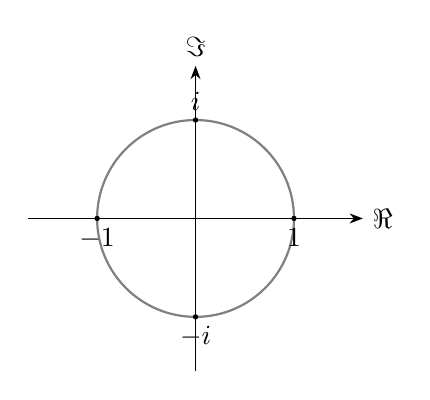
\begin{tikzpicture}[scale=1.25, >=Stealth]
  \draw[gray, thick] (0,0) circle (1);
  \draw[->] (-1.7,0) -- (1.7,0) node[right] {$\Re$};
  \draw[->] (0,-1.55) -- (0,1.55) node[above] {$\Im$};
  \filldraw (-1,0) circle (0.6pt) node[below] {$-1$};
  \filldraw (1,0) circle (0.6pt) node[below] {$1$};
  \filldraw (0,1) circle (0.6pt) node[above] {$i$};
  \filldraw (0,-1) circle (0.6pt) node[below] {$-i$};
\end{tikzpicture}
{\small (a) the complex-plane view: standard $\Re$/$\Im$ axes, $\pm1$, $\pm i$, unit circle}
\end{minipage}\hfill
\begin{minipage}[t]{0.48\textwidth}\centering
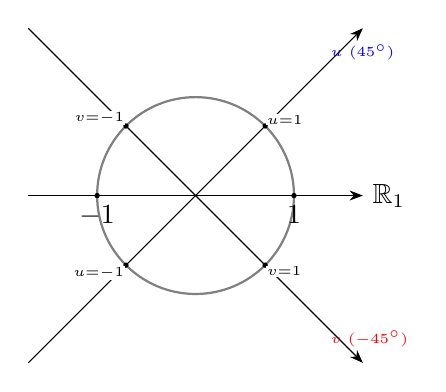
\begin{tikzpicture}[scale=1.25, >=Stealth]
  \draw[gray, thick] (0,0) circle (1);
  \draw[->] (-1.7,0) -- (1.7,0) node[right] {$\R_1$};
  \draw[->] (-1.7,-1.7) -- (1.7,1.7) node[very near end, above right, font=\tiny, blue] {$u$ ($45^\circ$)};
  \draw[->] (-1.7,1.7) -- (1.7,-1.7) node[very near end, below right, font=\tiny, red] {$v$ ($-45^\circ$)};
  \filldraw (-1,0) circle (0.6pt) node[below] {$-1$};
  \filldraw (1,0) circle (0.6pt) node[below] {$1$};
  \filldraw (0.707,0.707) circle (0.6pt) node[above right, font=\tiny, fill=white, inner sep=0.5pt] {$u{=}1$};
  \filldraw (-0.707,-0.707) circle (0.6pt) node[below left, font=\tiny, fill=white, inner sep=0.5pt] {$u{=}{-}1$};
  \filldraw (0.707,-0.707) circle (0.6pt) node[below right, font=\tiny, fill=white, inner sep=0.5pt] {$v{=}1$};
  \filldraw (-0.707,0.707) circle (0.6pt) node[above left, font=\tiny, fill=white, inner sep=0.5pt] {$v{=}{-}1$};
\end{tikzpicture}
{\small (b) the same circle in the $\pm45^\circ$-rotated frame: $u$/$v$ axes with the unit points $u{=}\pm1$, $v{=}\pm1$}
\end{minipage}\par\vspace{8pt}
\begin{minipage}[t]{0.48\textwidth}\centering
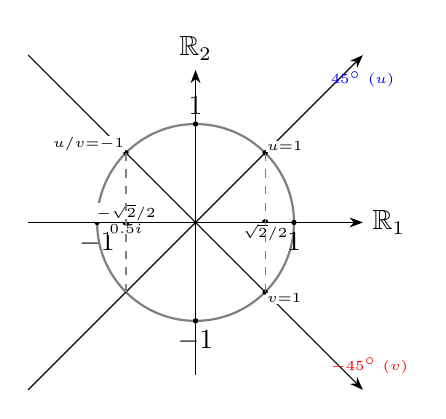
\begin{tikzpicture}[scale=1.25, >=Stealth]
  \draw[gray, thick] (0,0) circle (1);
  \draw[->] (-1.7,0) -- (1.7,0) node[right] {$\R_1$};
  \draw[->] (0,-1.55) -- (0,1.55) node[above] {$\R_2$};
  \filldraw (-1,0) circle (0.6pt) node[below] {$-1$};
  \filldraw (1,0) circle (0.6pt) node[below] {$1$};
  \filldraw (0,1) circle (0.6pt) node[above] {$1$};
  \filldraw (0,-1) circle (0.6pt) node[below] {$-1$};
  \draw[->] (-1.7,-1.7) -- (1.7,1.7) node[very near end, above right, font=\tiny, blue] {$45^\circ\ (u)$};
  \draw[->] (-1.7,1.7) -- (1.7,-1.7) node[very near end, below right, font=\tiny, red] {$-45^\circ\ (v)$};
  % 轴无数字刻度: 每轴只有一个单位点 1 (pat: 所有轴都是 1)
  \filldraw (-0.707,0) circle (0.8pt) node[below, font=\tiny, fill=white, inner sep=0.5pt] {$0.5i$};
  \filldraw (-0.707,0) circle (0.8pt) node[above, font=\tiny, fill=white, inner sep=0.5pt] {$-\sqrt2/2$};
  \filldraw (0.707,0) circle (0.8pt) node[below, font=\tiny, fill=white, inner sep=0.5pt] {$\sqrt2/2$};
  \filldraw (0.707,0.707) circle (0.6pt) node[above right, font=\tiny, fill=white, inner sep=0.5pt] {$u{=}1$};
  \filldraw (0.707,-0.707) circle (0.6pt) node[below right, font=\tiny, fill=white, inner sep=0.5pt] {$v{=}1$};
  \filldraw (-0.707,0.707) circle (0.6pt) node[above left, font=\tiny, fill=white, inner sep=0.5pt] {$u/v{=}{-}1$};
  \draw[dashed, gray] (0.707,0.707) -- (0.707,0);
  \draw[dashed, gray] (0.707,-0.707) -- (0.707,0);
  \draw[dashed, gray] (-0.707,0.707) -- (-0.707,0);
  \draw[dashed, gray] (-0.707,-0.707) -- (-0.707,0);
\end{tikzpicture}
{\small (c) pat: the $u$/$v$ axes (unit $1$, no numbers on them); pat values on the real axis: $\sqrt2/2$ (the $+1$ reading) and $0.5i$ (the $-1$ reading, the arm's vertical component --- the negative-side convention), with the perpendicular drops at $\pm\sqrt2/2$}
\end{minipage}\hfill
\begin{minipage}[t]{0.48\textwidth}\centering
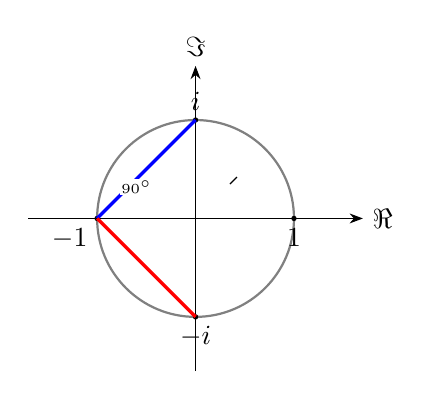
\begin{tikzpicture}[scale=1.25, >=Stealth]
  \draw[gray, thick] (0,0) circle (1);
  \draw[->] (-1.7,0) -- (1.7,0) node[right] {$\Re$};
  \draw[->] (0,-1.55) -- (0,1.55) node[above] {$\Im$};
  \filldraw (-1,0) circle (0.6pt) node[below left] {$-1$};
  \filldraw (1,0) circle (0.6pt) node[below] {$1$};
  \filldraw (0,1) circle (0.6pt) node[above] {$i$};
  \filldraw (0,-1) circle (0.6pt) node[below] {$-i$};
  \draw[very thick, blue] (-1,0) -- (0,1);
  \draw[very thick, red] (-1,0) -- (0,-1);
  \draw (0.35,0.35) -- (0.42,0.42);
  \node[font=\tiny, fill=white, inner sep=0.5pt] at (-0.6,0.32) {$90^\circ$};
\end{tikzpicture}
{\small (d) the $90^\circ$ fold from $-1$: the two straight arms end at $\pm i$ (machine-verified fold vertices --- the fold spans the imaginary axis)}
\end{minipage}
% TODO (visualization): the four renderings above are schematic TikZ sketches;
% refined rendering (colors, mapping arrows, 3D shading) is planned with a
% vision-capable AI pass; the mathematical content is fixed by the verified
% statements of Part IV.
\caption{The same unit circle, four readings: (a) the complex-plane
view (standard $\Re$/$\Im$ axes, $\pm1$, $\pm i$); (b) the same circle in
the $\pm45^\circ$-rotated frame --- the $u$/$v$ axes with the unit points
$u{=}\pm1$, $v{=}\pm1$ (same circle, different axes); (c) pat: the
$u$/$v$ axes carry the unit $1$ only, and every value appears on the
real axis by perpendicular projection --- the pat values read are
$\sqrt2/2$ for the $+1$ reading and $0.5i$ for the $-1$ reading (the
arm's vertical component, the negative-side convention), the drops
landing at $\pm\sqrt2/2$, straight lines; (d) the $90^\circ$ fold from $-1$: the two straight arms end
at $\pm i$ (machine-verified fold vertices; the fold spans the
imaginary axis). Radius $1$ throughout; schematic,
refined rendering forthcoming.}
\label{fig:four_views}
\end{figure}

The question is not answered by the framework; it is only made precise.
The standard definitions of $i$ and of the irrational numbers are the
axiomatic base of mathlib (the ZFC framework), and this paper does not
contest them: the fold construction of \S\ref{sec:partIV:fold} is a
presentation of the standard complex plane, not an alternative to it.
The choice recorded here is the author's presentation choice: between a
complex axis \emph{folded by $90^\circ$ that preserves the dimension}
(the fold of this paper) and a native straight axis that would raise the
dimension again, the author chooses the fold --- a straight native axis
would add nothing to the verified chain of the earlier parts, while the
fold makes the projection asymmetry visible and machine-verifiable.

\subsection{The two readings are symmetric: the right-isosceles triangle pair}
\label{sec:partIV:tri}

The four readings of Figure~\ref{fig:four_views} leave two readings of
the same object, and the machine verifies that they carry identical
data --- the same pair of right-isosceles triangles, once read by
length, once read by value (\texttt{EulerFoldImagAxis.lean}, 12 new
declarations, 0 \texttt{sorry}, build green):
\begin{itemize}
\item \emph{The length reading ($T_1$).} The triangle
  $\{0,(1+i)/2,(1-i)/2\}$ has the right angle at $0$
  (\texttt{fold\_tri\_right\_angle}), legs
  $\|(1\pm i)/2\|=\sqrt2/2$ (\texttt{fold\_tri\_leg1},
  \texttt{fold\_tri\_leg2}), hypotenuse $\|i\|=1$
  (\texttt{fold\_tri\_hyp}), and Pythagoras
  $(\sqrt2/2)^2+(\sqrt2/2)^2=1^2$
  (\texttt{fold\_tri\_pythagorean}).
\item \emph{The value reading ($T_2$).} The triangle
  $\{0,-1,(-1\pm i)/2\}$ has hypotenuse $[0,-1]$ --- the value $-1$
  on the real axis (\texttt{fold\_tri\_minus\_hyp}), right angle at
  the fold-arm midpoint $(-1\pm i)/2$
  (\texttt{fold\_tri\_minus\_right\_angle}), and legs of length
  $\sqrt2/2$ (\texttt{fold\_tri\_apex\_norm},
  \texttt{fold\_tri\_apex\_to\_neg\_one}).
\item \emph{Two readings of one leg.} Each leg has length
  $\sqrt2/2$ (length reading) and vertical component $1/2$, read as
  $0.5i$ (value reading) (\texttt{fold\_tri\_arm\_im}); the two arms
  sum to the unit, $(1+i)/2+(-1+i)/2=i$, i.e.\ $0.5i+0.5i=i$
  (\texttt{fold\_tri\_arms\_sum}), and $i\cdot i=-1$
  (\texttt{fold\_tri\_value\_square}): the value chain closes on the
  negative side. The symmetry of $\pm i$ and $\pm\sqrt2/2$ is
  therefore not a visual impression: $\pm i$ are the two fold arms
  of length $\sqrt2/2$ whose vertical components are $\pm 0.5i$.
\end{itemize}

\paragraph{The displayed divergence.} The same pair displays the
divergence of the two notations, and the author records it with the
two machine outcomes side by side. In the $\sqrt2/2$ reading the
statements build and are verified (the 12 declarations above, plus
the value-side anchors of \S\ref{sec:partIV:route}). In the $i$ reading
the same statements either do not type or are false; the isolated
probe \texttt{ProbeFailTriSymm.lean} (outside the library, not part
of the build; output in
\texttt{ProbeFailTriSymm.errors.txt}) captures:
\begin{itemize}
\item \emph{No type.} $u=i$ (\texttt{Complex.I}) fails with
  \texttt{Type mismatch: Complex.I has type $\mathbb C$, is expected
  to have type $\mathbb C\to\mathbb R$} --- the reading is a
  real-valued function, the imaginary unit a complex number; and
  $u(z)=i$ is silently coerced to $\uparrow u(z)=i$, a false
  real-equals-imaginary statement that no proof can close;
\item \emph{False Pythagorean.} $(0.5i)^2+(0.5i)^2=(-1)^2$ is
  rejected: the left side is $-1/2$, not $1$;
\item \emph{Not an identity.} $i=\sqrt2/2$ as elements is false
  ($0\neq\sqrt2/2$) --- the two readings are a dictionary, not an
  equality of types.
\end{itemize}

The same divergence is reproduced in the transformer. In the
two-pole experiments of \cite{fourtheorems} (the same 45-run program,
reproduced in the self-contained package at the cited DOI, including
the training runtime, the experiment code, and the outputs), the
symmetry-center experiments (E14) pass in-representation on all three
groups (10/10, 72/72, 24/24), and the strict-transfer experiments
(E15) give $26/26$ on the in-representation pole and $0/26$ on the
cross-representation pole --- the same object keeps one of the two,
symmetry or mapping, not both; the equivalence-statement bridge restores
part of the pole ($16/26$, $25/26$, $15/26$). The symmetry of the fold
arms and the mapping to $i$ are thus, in both the machine and the
experimental record, alternatives: one of the two holds, and declaring
the equivalence is the way to keep both.

\paragraph{The author's hypothesis, and the boundary of the claim.}
The author records the following as a hypothesis, not as a proven
claim: if $\pm i$ and $\pm\sqrt2/2$ are two readings of one symmetric
object (as the verified triangle pair states), then the divergence
displayed is a divergence \emph{of the presentations themselves} ---
of what each reading can even express, the type failures being
constraints of the statement space rather than cosmetic differences
--- while the underlying object remains one (the hypothesis). The
author takes the presentation to be a part of the logical structure:
an ill-typed claim is not a claim, and the statement space of a
presentation decides which construction routes are open at all; the
base-point criterion of \S\ref{sec:partIV:route} is such a
constraint: $\pi/2$-type constructions are not admissible inputs, and
the four axes carry no log-2 unit --- the $2\pi/\ln 2$ lattice of
\S\ref{sec:partIV:route} is the factor's separate single-prime
structure, not the scale of the four readings above; the
$\sqrt2/2$ reading still carries the
zero information of the critical
line in complete form (the weak projection value bridge of
\S\ref{sec:partIV:route}, \texttt{projection\_zero\_line\_complete}),
while the $i$-based statements fail in the native frame (as the probe
captures). The author does not
draw the further conclusion: whether the counting bridge of the value
side closes --- in either notation --- remains the open gap of
\S\ref{sec:partIV:route}; what the machine records is exactly the
pair above: 12 declarations build, the $i$ statements fail; the
symmetry and the $i$-mapping do not coexist in the same system.

\subsection{The false-real-axis extension}
\label{sec:partIV:fra}

The false-real-axis framework of \S\ref{sec:L8} (no zeros for
$\Re s<0$, real-valuedness on the real axis) is extended to the
base-point $e^{\pi/4}$: the T-coordinate first-order restatement
(\texttt{TCoordOffline.lean}, 10 theorems, machine-verified) gives the
three-level criterion $|T|^2\ne 1$, the first-order position difference
$1-2\Re\rho\ne 0$, the odd/even common-zero structure, and the
difference-structure non-vanishing $2^\rho\ne 1$. These are the
order-reduction pieces of the route: they hold uniformly in the strip
and are compatible with the off-line assumption.

\subsection{The Euler-circle fold: the imaginary axis as a $90^\circ$ fold}
\label{sec:partIV:fold}

We construct the imaginary axis from the negative side of the Euler
circle, as a $90^\circ$ orthogonal fold, using only the net elements
of the framework (machine-verified, \texttt{EulerFoldImagAxis.lean}):
the Euler identity $e^{i\pi}=-1$ (negative-side basepoint), the
rotation $(-1)\cdot e^{\mp i\pi/2}=\pm i$ (the imaginary units, from
$\exp$ additivity and the $2\pi$ period), the fold directions
$\arg(1\pm i)=\pm\pi/4$ (from the tangent of the sum), the $90^\circ$
orthogonality (inner product zero and direction difference $\pi/2$),
the length $\|1\pm i\|=\sqrt2$, and the polar form
$e^{\pm i\pi/4}=\frac{\sqrt2}{2}(1\pm i)$ (the $45^\circ$ basis).
Every step is a standard fact of complex geometry, re-narrated on the
fold; no axiom is added.

\begin{theorem}[The fold is the imaginary axis]
\label{thm:fold_imag_axis}
The two rays from $-1$ at angles $\pm\pi/4$ form a fold whose endpoints
are the imaginary units (\texttt{fold\_vertices\_are\_imag\_units});
the fold spans the imaginary axis
(\texttt{imag\_axis\_eq\_span\_fold\_vertices}); the fold coordinates
are a linear coordinate system of $\mathbb C$
(\texttt{foldCoordHomeo}); and the straightening of the fold is a
homeomorphism of $\mathbb R$ onto the fold set
(\texttt{foldArcHomeo}), with arc-length preservation on each arm
(\texttt{foldArc\_dist\_pos}, \texttt{foldArc\_dist\_neg}) and unit
speed (\texttt{foldArc\_hasDerivAt\_pos},
\texttt{foldArc\_hasDerivAt\_neg}). The fold is the imaginary axis
viewed from the negative side: the same axis that classical geometry
obtains by rotating the real axis by $90^\circ$ (the geometric
representation of Argand \cite{argand1806}; the Euler identity
\cite{euler1748}).
\end{theorem}

The construction is a presentation-layer statement in the sense of
\S\ref{sec:methodology}: every step is a standard fact (Euler's
identity, polar coordinates, rotations), the fold is a re-narration of
the imaginary axis, and the honest boundary is that no new mathematics
is claimed --- the value is the explicit geometry, which the next
subsection turns into coordinate bridges.

\subsection{The fold coordinate bridges}
\label{sec:partIV:bridges}

The fold coordinates make four standard structures explicit as
coordinate lines (all machine-verified, 0 \texttt{sorry}):
\begin{itemize}
\item \emph{Conjugation is the coordinate swap.}
  $\texttt{fold\_conj\_swap}$: $\texttt{foldCoordFromC}(\bar z)$ is the
  swapped pair of $\texttt{foldCoordFromC}(z)$ --- the real-axis
  reflection is the exchange of the two $45^\circ$ half-axes;
\item \emph{The imaginary axis is the diagonal.}
  $\texttt{fold\_imag\_axis\_diag}$: $\Re z=0\iff u+v=0$;
\item \emph{The critical line is a horizontal line.}
  $\texttt{fold\_critical\_line\_horiz}$:
  $\Re z=\tfrac12\iff u+v=\sqrt2/2$;
\item \emph{Real values are the fixed line of the swap.}
  $\texttt{fold\_real\_iff\_swap\_fixed}$: $\Im z=0\iff u=v$.
\end{itemize}
These bridges are the logical-completeness requirement of the new
frame: any node of the chain re-stated in fold coordinates must pass
through the bridges, so that the two presentations cannot diverge. The
Riemann nodes themselves are not re-proved (a linear change of
coordinates translates every analytic statement automatically); only
the translations are verified.


\subsection{The symmetry elements in fold coordinates}
\label{sec:partIV:sym}

The symmetry family of the chain (Layer~2's zero reflection, Layer~8's
conjugation, the critical-line fixed-point character) takes an explicit
form in fold coordinates; all statements of this subsection are
machine-verified (0 \texttt{sorry}).
\begin{itemize}
\item \emph{Conjugation is the coordinate swap.}
  (\texttt{fold\_conj\_swap}, \S\ref{sec:partIV:bridges}):
  $(u,v)\mapsto(v,u)$.
\item \emph{Reflection $s\mapsto 1-s$ is the mirror shift.}
  (\texttt{fold\_reflection\_mirror\_u}, \texttt{fold\_reflection\_mirror\_v}):
  \begin{equation}
    u(1-s)=\tfrac{\sqrt2}{2}-u(s),\qquad
    v(1-s)=\tfrac{\sqrt2}{2}-v(s).
  \end{equation}
  The reflection reflects each fold coordinate about the midpoint
  $\sqrt2/4$; the critical line $u+v=\sqrt2/2$ is its fixed line.
\item \emph{Conjugation preserves the fold critical line.}
  (\texttt{fold\_critical\_conj}): the swap leaves $u+v=\sqrt2/2$
  invariant --- the fold-critical-line statement of
  \S\ref{sec:partIV:bridges} holds for $\bar z$ iff it holds for $z$.
\item \emph{On the fold critical line, reflection equals conjugation.}
  (\texttt{fold\_reflection\_eq\_conj\_on\_line}): under
  $u+v=\sqrt2/2$ the mirror shift and the swap coincide --- the
  classical fixed-point character of the critical line
  (\texttt{critical\_line\_iff\_reflect\_fixed} of the chain) in fold
  form.
\end{itemize}
The two symmetry operations of the chain --- conjugation and the zero
reflection --- are therefore, in the fold frame, two variants of the
same coordinate operation: a swap, with the reflection adding a shift
that vanishes exactly on the critical line. The reflection pairing of
an off-line zero $\rho$ (its orbit
$\{\rho,\bar\rho,1-\rho,1-\bar\rho\}$ of \S\ref{sec:partIII:fail})
reads in fold coordinates as the orbit of $(u,v)$ under the two
operations
$(u,v)\mapsto(v,u)$ and $(u,v)\mapsto(\tfrac{\sqrt2}{2}-u,\tfrac{\sqrt2}{2}-v)$:
a swap and a mirror shift. This is the presentation-layer content of
the symmetry family; it changes no statement of the chain and adds no
axiom.

\subsection{The odd/even observation route}
\label{sec:partIV:route}

\emph{Observation protocol.} The observation of this section uses a
single carrier topology: the $V$-fold with a single opening direction
(the opening toward the strip, i.e.\ the direction of the critical line
$u+v=\sqrt2/2$), together with the complex axis as reference. The
choice is a presentation choice, and it is complete: the observed
quantities (phase differences, winding numbers, projected integrals)
are quantities of the complex plane, not of the carrier; observation
paths are homotopy-independent (Cauchy--Goursat, machine-verified in
\S\ref{sec:partII} and the ring-shrinking theorems); and the singular off-line orbit
of \S\ref{sec:partIII:fail} is a fact of the plane, present in every
carrier. The three carrier topologies (the $V$-fold $\cong\mathbb R$,
the closed loop $\cong S^1$, the two disjoint half-axes $\cong
\mathbb R\sqcup\mathbb R$) therefore need not all be observed: their
classification is a presentation statement, and one carrier with a
single opening direction --- the fold toward the strip --- suffices.

\emph{The observation plane: the critical line $\times$ $z$.}
The observation of this section is performed on a plane that is
\emph{not} the complex plane: it is the plane spanned by the critical
line itself and a direction $z$ orthogonal to the complex plane --- the
two planes share the critical line and meet at right angles. In fold
coordinates the two observation axes are:
\begin{itemize}
\item \emph{Axis 1 is the critical line itself} (after precise
  base-point migration, the critical line becomes the observation
  axis): its reading is $\sqrt2\,\Im s$
  (\texttt{obs\_axis1\_is\_critical\_direction}) --- the position along
  the line, the information that is declared irrelevant and dropped;
  equivalently, the observation point of axis~2 is the critical line,
  the reflection fixed line $s=1-\bar s$
  (\texttt{obs\_axis1\_reflect\_fixed});
\item \emph{Axis 2 is orthogonal to the critical line}: its reading is
  $\sqrt2(\Re s-\tfrac12)$
  (\texttt{obs\_axis2\_is\_distance}) --- the distance from the critical
  line, the information that is kept.
\end{itemize}
The projection requirement is machine-verified: the critical line
projects to the single point $0$ on axis~2
(\texttt{critical\_projects\_to\_axis2\_point}), and \emph{only} the
critical line projects to that point
(\texttt{only\_critical\_projects\_to\_point}: the reading is $0$ iff
$\Re s=\tfrac12$). The base-point inversion closes the protocol: the
reading determines the abscissa uniquely
(\texttt{fold\_obs\_residual\_unique}) --- the observation object is
recovered from the reading, in the form of
\texttt{basepoint\_from\_residual} of the base-point migration family.

\emph{The self-reference of the odd/even split.} The route proposed for
the boundary of Part~III is: migrate the base-point to $e^{\pi/4}$ (the
$45^\circ$ direction, which is the fold arm), split into odd/even parts,
and observe the difference structure. The observation meets a
self-reference: at a zero $\rho$, the individual odd and even parts both
vanish (they share the zero --- $O_2(\rho)=E_2(\rho)=0$, machine-verified
in \S\ref{sec:partIII:fail}), so the single-lift ratio $O_2/E_2$ is the
indeterminate $0/0$ at the very point to be observed: the observation
function is zero at the observation point. The split resolves this
self-reference through the \emph{difference structure}: the phase ratio
$u_O/u_E=(2^s-1)/\|2^s-1\|$ is well defined at every zero
($2^\rho\ne 1$ in the strip, machine-verified), it is a unit complex
number --- a point of the Euler circle
(\texttt{FoldObservation.lean}: \texttt{phase\_ratio\_denom\_ne\_zero},
\texttt{phase\_ratio\_unit}) --- and in the fold coordinates of this
part it is read as the coordinate pair
$(u,v)=(\frac{\sqrt2}{2}(\Re+\Im),\frac{\sqrt2}{2}(\Re-\Im))$ of that
point (\texttt{phase\_ratio\_fold\_coords}), a well-defined reading with
no $0/0$. The resolution is machine-verified as a whole:
\texttt{self\_reference\_resolved} states that at a zero $\rho$ the
single-lift denominators both vanish ($\|O_2(\rho)\|=\|E_2(\rho)\|=0$,
the shared zero --- the self-reference), while the difference-structure
denominator does not ($\|2^\rho-1\|\ne 0$); and in the strip the
observation is well defined everywhere
(\texttt{observation\_well\_defined\_in\_strip}). The observation of
the phase ratio is therefore the reading of a point on the Euler circle
in fold coordinates --- the frame in which the imaginary axis is a fold
and conjugation is a swap. The machine-verified pieces are in place:
the false-real-axis access (\S\ref{sec:partIV:fra}), the non-singular
difference structure of \S\ref{sec:partIII:fail}
(\texttt{odd\_even\_phase\_ratio} is well defined at every zero), the
unit-circle character of the ratio (\texttt{phase\_ratio\_unit}), and
the fold frame itself (this part). What is \emph{not} in place is the
observation step: how the phase ratio --- an explicit function of $s$
alone --- is made to carry information about a hypothetical off-line
zero $\rho$. The ratio is
rigid but information-free for $\zt$ (machine-verified,
\S\ref{sec:partIII:fail}); the open question is whether the fold frame
supplies a second rigid quantity that, together with the ratio, forms a
generator ($G_1$ or $G_2$, \S\ref{sec:partIII:arch}). This is the
current work; its status is recorded honestly: verified infrastructure,
open observation step.

\par\emph{The projection value bridge: weak assertion (machine-verified).}
\emph{Definitions.} Throughout this paragraph: $u(s)$, $v(s)$ are the
fold coordinates of the \emph{argument} $s$ of \S\ref{sec:partIV:fold}
($u=\frac{\sqrt2}{2}(\Re s+\Im s)$, $v=\frac{\sqrt2}{2}(\Re s-\Im s)$);
$d(s):=\texttt{foldObsProj}(s)=u(s)+v(s)-\frac{\sqrt2}{2}
=\sqrt2(\Re s-\frac12)$ is the axis-2 reading of the observation plane
of \S\ref{sec:partIV:route} (the preimage of $0$ is exactly the critical
line); and $U:=\texttt{zetaFoldU}$, $V:=\texttt{zetaFoldV}$ are the fold
components of the \emph{value} $\zt(s)$ (the same formula applied to the
value, $U=\frac{\sqrt2}{2}(\Re\zt+\Im\zt)$,
$V=\frac{\sqrt2}{2}(\Re\zt-\Im\zt)$).
\par The bridge required is deliberately weak: the author's framing
answers the open step above in the weak sense --- after the projection
drops axis~1, the remaining information is \emph{complete} for the
judgement ``the zero is on the critical line''. No full value bridge is
sought --- no counting, winding, or flip correlation. The author's
reason is structural and presentation-independent: the counting
identity is the target in another guise --- the number of in-strip
zeros equals the number of on-line zeros \emph{is} the claim itself
--- so a counting bridge would be circular, and the strong variants
through a value function are excluded by the self-reference-free
design of the observation quantity $d$, which does not depend on
$\zt$ (\texttt{foldObsProj\_independent\_of\_zeta}). Two pieces are
machine-verified. First, the value-domain anchors:
\begin{equation}
  U+V=\sqrt2\,\Re\zt(\cdot),\qquad U-V=\sqrt2\,\Im\zt(\cdot)
  \qquad (\texttt{zeta\_fold\_sum\_re}, \texttt{zeta\_fold\_diff\_im}),
\end{equation}
together with the immediate corollary that $\zt(\rho)=0$ implies both
anchors vanish (\texttt{zeta\_fold\_dual\_proj\_zero\_of\_zero}): the
vanishing of $\zt$ is characterised completely by the dual anchors.
Second, the weak assertion itself
(\texttt{projection\_zero\_line\_complete}): for a zero $\rho$ of the
strip,
\begin{equation}
  \rho\in\text{critical line}
    \iff d(\rho)=0
    \iff \bigl(U(\rho)=0\wedge V(\rho)=0\wedge d(\rho)=0\bigr).
\end{equation}
Every input of the target judgement --- zero-ness in the value-domain
anchors, on-line-ness in $d$ --- lies in the projection quantities;
axis~1 (the position $\sqrt2\,\Im s$ along the critical line) is not
used. Projection is therefore complete for the judgement it was built
for, and the discarded information is exactly the information the
judgement does not need.
Both pieces rest on native equivalences of the fold frame,
machine-verified without reference to $i$ or $\pi$
(\texttt{NativeAxisEquiv.lean}). With the constant
$c=\sqrt2/2=2^{-1/2}$ --- the $45^\circ$ fold constant --- the fold
coordinates $u$, $v$ recover
the standard coordinates natively,
\begin{equation}
  \frac{u+v}{\sqrt2}=\Re z\,,\qquad \frac{u-v}{\sqrt2}=\Im z
  \qquad (\texttt{axis\_recovery\_re}, \texttt{axis\_recovery\_im}),
\end{equation}
uniquely (\texttt{axis\_unique}) and with the modulus preserved
($u^2+v^2=(\Re z)^2+(\Im z)^2$;
\texttt{axis\_norm\_sq\_preserving}); the underlying algebra is the
real linear bijection $c\,[[1,1],[1,-1]]$ of determinant $-1$. The
surjectivity direction (\texttt{axis\_exists}) only re-assembles the
Lean $\mathbb C$ container from the standard coordinates --- a
read-back presentation with no $i$-transformation semantics and no
dependence on any $\zt$-related theorem. The author's base-point
criterion is thus respected: the imaginary unit occurs only in that
read-back layer, and $\pi/2$-type constructions are not inputs of the
observation frame (the author's original identification of these axes
with the framework's log axes, and the log-2 base-point scale, were
withdrawn as a cognitive error; see the AI-contribution statement).

\paragraph{Analytic restatement of the observation.}
For readers who prefer the analytic language, the observation of this
section is a single continuous function. Define
\begin{equation}
  d(s)=\texttt{foldObsProj}(s)=u(s)+v(s)-\tfrac{\sqrt2}{2}
    =\sqrt2\,\bigl(\Re s-\tfrac12\bigr),
\end{equation}
the (rescaled) distance from the critical line. Then:
\begin{itemize}
\item $d$ is continuous (\texttt{fold\_obs\_proj\_continuous}, from the
  continuity of the fold coordinates);
\item the critical line is exactly the zero set of $d$
  (\texttt{fold\_obs\_proj\_zero\_set}): $d(s)=0\iff\Re s=\tfrac12$;
\item the zero judgement is a function value: for a zero $\rho$ of
  $\zt$, $\rho$ lies on the critical line iff $d(\rho)=0$ --- a
  pointwise reading, with no path, no contour, no winding number.
\end{itemize}
The comparison with the homotopy (contour) language is deliberate. The
winding-number judgement of \S\ref{sec:partII} requires a path on which
$\zt\ne 0$; at the boundary of Part~III this input fails structurally
(the off-line orbit is all zeros, \S\ref{sec:partIII:fail}). The
function $d$ carries no such precondition: it does not mention $\zt$
at all (\texttt{foldObsProj\_independent\_of\_zeta}), so the pointwise
judgement $d(\rho)=0$ is never blocked by a singular path. The price is
the honest boundary already recorded: a function that does not mention
$\zt$ carries no information about $\rho$ itself (the object-level
self-reference of \S\ref{sec:partIII:honest} is untouched). The
analytic restatement is a presentation-layer reformulation --- standard
facts (the $\Re$ projection, the critical-line equation, continuity of
coordinate functions) re-stated on the fold; it is not new mathematics,
and it adds no axiom. Methodologically, the observation protocol is an
organization of classical principles --- structure-preserving
coordinates (the fold, a linear coordinate change), declared-loss
projection (axis~2 kept, axis~1 declared irrelevant and dropped, with
faithfulness verified), and base-point inversion (the reading determines
the abscissa uniquely) --- into a single protocol whose contribution is
the organization and the verified faithfulness, not the principles
themselves, which are standard.

\paragraph{Reconstructing $\zt$ in the fold frame (dimension lifting).}
The observation of the previous paragraphs is information-free for
$\zt$ by design ($d$ does not mention $\zt$). The fold frame also
offers the opposite direction: reconstruct $\zt$ itself in fold
coordinates. Write, as in the weak-assertion paragraph above,
\begin{equation}
  U(s)=\texttt{zetaFoldU}(s)=u(\zt(s)),\qquad
  V(s)=\texttt{zetaFoldV}(s)=v(\zt(s)),
\end{equation}
the two real components of $\zt(s)$ along the two arms of the fold
(the $\pm45^\circ$ directions). The reconstruction is a presentation,
not a loss: the pair $(U(s),V(s))$ determines $\zt(s)$ back, through
the inverse of the fold coordinate map
(\texttt{zeta\_fold\_invertible}: \texttt{foldCoordToC}\,$(U,V)=\zt$).
Nothing is lost --- in contrast to the observation projection $d$ and
the phase ratio, which are information-free by construction. The zero
judgement takes the joint form: $\zt(\rho)=0$ iff $U(\rho)=0$ and
$V(\rho)=0$ (\texttt{zeta\_fold\_zero\_iff}) --- a two-component
reading, joint zero rather than ratio.

The symmetry elements of \S\ref{sec:partIV:sym} act on the components
as on any fold coordinates, and the conjugation bridge
(\S\ref{sec:partIV:bridges}) lifts to the reconstructed function:
$U(\bar s)=V(s)$ in the strip
(\texttt{zeta\_fold\_conj\_swap\_u}, \texttt{zeta\_fold\_conj\_swap\_v},
from the conjugation symmetry of $\zt$ composed with bridge~1, the
swap), and the zeros of a conjugate pair $\rho,\bar\rho$ are a pair of
joint zeros (\texttt{zeta\_fold\_conj\_zero\_pair}). The inversion of
the base-point family also admits a fold reading:
$u(1/s)=v(s)/\|s\|^2$ and symmetrically
(\texttt{fold\_inversion\_swap\_u}, \texttt{fold\_inversion\_swap\_v}):
inversion in fold coordinates is a swap plus a scaling (because
$1/s=\bar s/\|s\|^2$), joining the three symmetry operations of the
frame --- conjugation (a pure swap), reflection (a mirror translation),
inversion (a swap plus a scaling).

Two rigidity facts follow for an off-line zero $\rho$ inside the
critical circle (\S\ref{sec:partIV:fra}). First, $\zt(1/\rho)\ne 0$:
inversion maps the point into the convergence region $\Re s\ge1$,
where $\zt$ has no zeros (machine-verified,
\texttt{offline\_inversion\_nonzero}, via the Euler product). Second,
therefore, the inverted point is not a zero, and its fold components
are not jointly zero (\texttt{zeta\_fold\_inversion\_nonzero}) --- in
contrast with $\rho$ itself, whose components are jointly zero. The
two facts form a comparison, not a contradiction: the components of
the inverted point carry the non-vanishing of $\zt(1/\rho)$, while the
components of $\rho$ carry the vanishing of $\zt(\rho)$; nothing
transfers the vanishing from one point to the other, because there is
no value bridge for $\zt$ under inversion --- inversion does not
preserve zeros. This is the precise form of generator gap~(ii) of
\S\ref{sec:partIII:arch}: the reconstructed components carry the
information of $\zt$ (invertibly), but the generator still needs a
mechanism that tracks zero-ness under the symmetry operations of the
frame. The status is recorded honestly: the reconstruction, the
symmetry lifting, and the two rigidity facts are machine-verified
(\texttt{FoldObservation.lean}, 90 declarations, no axioms); the value
bridge is open.

\paragraph{The reflection in fold components, and the joint observation.}
The reflection $s\mapsto 1-s$ admits a fold reading as well: with the
functional-equation multiplier
\begin{equation}
  m(s)=\texttt{zetaReflectMul}(s)=2(2\pi)^{-s}\Gamma(s)\cos\tfrac{\pi s}{2},
  \qquad \zt(1-s)=m(s)\,\zt(s),
\end{equation}
one has
\begin{equation}
  U(1-s)=\Re m(s)\cdot U(s)+\Im m(s)\cdot V(s),\qquad
  V(1-s)=\Re m(s)\cdot V(s)-\Im m(s)\cdot U(s)
\end{equation}
(\texttt{zeta\_fold\_reflect\_u}, \texttt{zeta\_fold\_reflect\_v}): the
reflection acts on the components by the multiplier matrix
$\bigl(\begin{smallmatrix}a&b\\-b&a\end{smallmatrix}\bigr)$, $a=\Re m$,
$b=\Im m$, a rotation--scaling. The three symmetry operations of the
frame now have their complete fold-component forms: conjugation is a
pure swap, reflection is a rotation--scaling by the multiplier matrix,
inversion is a swap plus a scaling. The fold modulus
$U(s)^2+V(s)^2=\|\zt(s)\|^2$ (\texttt{zeta\_fold\_norm\_sq} --- the
fold coordinates are a $45^\circ$ rotation and preserve the Euclidean
norm) scales by $\|m(s)\|^2$ under reflection
(\texttt{zeta\_fold\_reflect\_norm\_sq}); on the critical line
$\|m\|=1$, so the reflection is a pure rotation there. The reflection
pairs zeros: $\zt(\rho)=0$ in the strip gives jointly vanishing
components at $1-\rho$ (\texttt{zeta\_fold\_reflect\_zero\_pair}).

The observation plane of \S\ref{sec:partIV:route} and the
reconstruction of the previous paragraph join into one observation:
for an off-line zero $\rho$ inside the critical circle
(\S\ref{sec:partIV:fra}), the three readings are
\begin{equation}
  U(\rho)=V(\rho)=0,\qquad d(\rho)\ne 0,\qquad d(1/\rho)>0,
\end{equation}
machine-verified as a whole (\texttt{joint\_observation\_inversion}):
the components vanish jointly (the zero information), axis~2 rejects
the line (the off-line information, $d(\rho)\ne0$ by
\texttt{fold\_projection\_point\_iff\_critical}), and the inverted
point lies in the positive region of axis~2 ($d(1/\rho)>0$, because
inversion maps the circle into the convergence region $\Re s>1$,
\texttt{offline\_obs\_proj\_pos\_at\_inverse}; the axis-2 reading under
inversion is the coordinate fact
$d(1/s)=\sqrt2(\Re s/\|s\|^2-\tfrac12)$,
\texttt{fold\_obs\_proj\_inversion}). The joint observation is the
complete protocol in the presence of inversion: zero information lives
in the components (joint zero), position information lives in axis~2
(non-zero, and positive at the inverted point). The two families are
orthogonal --- the components do not know the axis-2 reading and
conversely --- and this orthogonality is the precise form of the open
value bridge: the joint observation records the two facts
($\rho$ zero and off-line) side by side without connecting them, and
nothing in the linear symmetry family can transfer the joint zero to
the axis readings (a linear map preserves the zero vector, so the
symmetry operations of the frame --- swaps, multiplier matrices, swaps
plus scalings --- cannot turn the vanishing of the components into
information about $d$). The honest conclusion of this paragraph: the
three symmetry operations do not constitute a zero-tracking mechanism;
the observation protocol is complete and machine-verified, and the
generator gap is unchanged.

\paragraph{The four directions of the fold axis.}
The fold axis is a $45^\circ$ axis with irrational scale
($\sqrt2/2$), not the axis system of the complex plane itself: it is
not ``$\zt$'s own'' coordinate frame. From its vertex the fold has
four directions --- the two arms, each with its two half-directions ---
and $\zt$ projects onto each half-arm separately. The four directional
components are defined by direct projection with half-arm truncation,
not through the coordinate pair $(U,V)$:
\begin{equation}
  u^+(s)=\max(\texttt{fold\_u}(\zt(s)),0),\qquad
  u^-(s)=\max(-\texttt{fold\_u}(\zt(s)),0),
\end{equation}
and symmetrically $v^+,v^-$ (\texttt{zetaFoldUPlus},
\texttt{zetaFoldUMinus}, \texttt{zetaFoldVPlus},
\texttt{zetaFoldVMinus}); each definition is a forward projection
(the max truncation is the geometry of the half-arm, not an inversion).
The four components are non-negative
(\texttt{zeta\_fold\_4direction\_nonneg}), and the zero judgement takes
the four-direction form: all four components vanish iff $\zt(s)=0$
(\texttt{zeta\_fold\_4direction\_zero\_iff}) --- at a zero the four
directions collapse together, since $0$ has no direction. Away from a
zero at least one component is positive
(\texttt{zeta\_fold\_4direction\_exists\_nonzero}), the pattern of
non-zero components being the direction sector of $\zt(s)$. The
reconstruction is a forward theorem, not an inversion: the four
components with their directions compose back to $\zt$,
\begin{equation}
  \zt(s)=\texttt{foldCoordToC}\,(u^+-u^-,\;v^+-v^-)
\end{equation}
(\texttt{zeta\_fold\_4direction\_reconstruct}, via the half-arm
cancellation $\max a\,0-\max(-a)\,0=a$,
\texttt{max\_sub\_neg\_max}) --- the cancellation of the two opposite
half-arms is part of the composition, and nothing is inferred back
from $\zt$ to the components. The four-direction presentation carries
exactly the information of the fold reconstruction (the components
with their directions determine $\zt$, and conversely), with the
direction attribution made explicit; and the direction attribution is
precisely what collapses at a zero. This is the directional form of
the self-reference: the four half-arm components of a zero are all
zero, and no direction survives.

\paragraph{The irrational axis and the eight components.}
The false complex plane of this part is, in essence, a
four-dimensional structure; the fold coordinate pair $(U,V)$ is only
half of it. The other half is carried by the odd/even phase ratio of
\S\ref{sec:partIII:fail},
\begin{equation}
  p(s)=\texttt{phaseRatio}(s)=\frac{2^s-1}{\|2^s-1\|},
\end{equation}
a unit complex number --- a point of the Euler circle --- defined
wherever $2^s\ne1$, in particular throughout the strip. The phase of
$p$ involves $\ln 2$ (irrational), and the singular set of $p$ is the
irrational-axis lattice $\{2\pi i k/\ln 2\}$ on the imaginary axis:
$p$ is the \emph{irrational-axis} half of the frame. In the
four-dimensional structure the two halves are the fold coordinates of
$\zt$ and of $p$,
\begin{equation}
  \bigl(u(\zt(s)),\;v(\zt(s)),\;u(p(s)),\;v(p(s))\bigr),
\end{equation}
and the eight half-arm components are the direction decomposition of
these four coordinates:
\begin{equation}
  u^\pm(\zt),\;v^\pm(\zt),\qquad u^\pm(p),\;v^\pm(p)
\end{equation}
(\texttt{zetaFoldUPlus}--\texttt{zetaFoldVMinus} for the $\zt$-side,
\texttt{phaseUPlus}--\texttt{phaseVMinus} for the $p$-side; each a
forward projection onto a half-arm, as in the previous paragraph).

The claim of this paragraph is that the irrational-axis half has been
\emph{absorbed into the base point and projected away}: the
conventional observation of $\zt$ uses only the $\zt$-side four
components, and the $p$-side --- the irrational-axis half --- is
discarded, because $p$ does not mention $\zt$. The $\zt$ function
therefore loses half of the four-dimensional frame, and this is the
seat of the self-reference: at a zero $\rho$ the $\zt$-side components
all vanish, and the observation collapses. The restoration of the lost
half is machine-verified: the $p$-side components do \emph{not}
collapse at a zero --- $p(\rho)$ is a unit complex number, its fold
modulus is $\|p(\rho)\|=1$, hence at least one of the four $p$-side
components is positive at $\rho$
(\texttt{phase\_4direction\_exists\_nonzero\_at\_zero}); the $p$-side
reconstruction is the allowed inverse, landing on the irrational-axis
side: $p(s)=\texttt{foldCoordToC}\,(p^+-p^-,\,q^+-q^-)$
(\texttt{phase\_4direction\_reconstruct}); and the eight-component
joint observation
\begin{equation}
  u^\pm(\zt(\rho))=v^\pm(\zt(\rho))=0,\qquad
  u^\pm(p(\rho))\vee v^\pm(p(\rho))\ne0
\end{equation}
is verified as a whole (\texttt{eight\_component\_observation}): at a
zero, the rational-axis half collapses and the irrational-axis half
receives the observation. The self-reference is broken in the sense
that the observation no longer vanishes at the observation point: the
eight-component frame is complete. The honest boundary is unchanged at
the value level: $p$ is an explicit function of $s$ and carries no
value of $\zt$, so the restored half is a complete \emph{observation}
frame, not a value bridge; the generator still needs the mechanism
that connects the two halves.

\paragraph{The odd/even structure and the locus of the value.}
The four-dimensional frame has an odd/even form which locates
precisely what the $p$-side does and does not carry. The odd and even
parts of the split are scaled copies of $\zt$
(\texttt{oddPart}\,$(s)=(1-2^{-s})\zt(s)$,
\texttt{evenPart}\,$(s)=2^{-s}\zt(s)$), so the four coordinates
$(u(O),v(O),u(E),v(E))$ are a linear embedding of the two
coordinates $(u(\zt),v(\zt))$ with explicit coefficients
(\texttt{odd\_fold\_u/v}, \texttt{even\_fold\_u/v}, via the
multiplication rule of \S\ref{sec:partIV:route}); and the merging is
invertible, $\zt(s)=O(s)+E(s)$ (\texttt{zeta\_odd\_even\_sum}). The
$p$-side shares the fold structure of the $\zt$-side: conjugation
passes through $p$, $p(\bar s)=\overline{p(s)}$
(\texttt{phase\_conj}, since $\ln 2$ is real), and the fold reading
swaps accordingly, $\texttt{fold\_u}(p(\bar s))=\texttt{fold\_v}(p(s))$
(\texttt{phase\_fold\_conj\_swap\_u}) --- the irrational-axis half
follows bridge~1 like the $\zt$-side.

The relative structure of the two halves is explicit: the modulus
ratio is
\begin{equation}
  \frac{\|O(s)\|}{\|E(s)\|}=\|2^s-1\|
\end{equation}
(\texttt{odd\_even\_norm\_ratio}), a function of $s$ alone. Hence of
the eight components, seven degrees of freedom --- the phase
difference, the modulus ratio, and the direction attribution --- are
explicit functions of $s$ (the $2^s$ factor structure); the only
degree of freedom that involves $\zt$ is the \emph{absolute scale}
$\|E(s)\|=2^{-\Re s}\|\zt(s)\|$. The value of $\zt$ is therefore
localised in a single quantity, the absolute scale, and this is where
the zero judgement lives: $\zt(\rho)=0$ iff the scale collapses.
The $p$-side provides the seven explicit degrees of freedom --- it
renders the observation complete and non-collapsing at a zero --- but
the zero information itself is the scale, and the scale is the
$\zt$-side. This is the precise locus of the value bridge: the
eight-component frame organises the seven explicit directions around
the one scale that carries $\zt$, and the generator must act on the
scale. Nothing in the present section moves the scale; the honest
statement is that the irrational-axis half, restored, surrounds the
value without touching it.

\paragraph{The scale and the Euler product: what the proof needs.}
The eighth degree of freedom --- the absolute scale --- is the
self-reference itself: the scale is the value of $\zt$, and the zero
judgement is the collapse of the scale. Its place inside the fold
frame is explicit: the scale is the square root of the fold modulus,
\begin{equation}
  \|\zt(s)\|=\sqrt{U(s)^2+V(s)^2}
\end{equation}
(\texttt{zeta\_scale\_sqrt}), and the scale collapses exactly when the
fold modulus does, $\|\zt(s)\|=0\iff U(s)=0\wedge V(s)=0$
(\texttt{zeta\_scale\_zero\_iff\_fold}) --- the zero judgement in scale
form. The restoration channel of the scale is the Euler product (the
prime axis), not the fold frame: in the convergence region,
\begin{equation}
  \|\zt(s)\|=\prod_p\|1-p^{-s}\|^{-1}\qquad(\Re s>1),
\end{equation}
the factor decomposition over all primes (machine-verified in its
finite-product form, \texttt{euler\_product\_bridge}); each prime
factor is non-zero in the convergence region and its fold components
do not vanish jointly
(\texttt{euler\_factor\_fold\_nonzero}) --- the prime axis enters the
fold frame factor by factor, the full spectrum $\ln p$ of which the
irrational axis $\ln 2$ is the single-prime case. The scale is
therefore not an object outside the frame: it is the fold modulus, and
its structure is the Euler product over all primes.

What the proof needs of the scale is a precise and honest statement.
The zero judgement needs the scale as \emph{input}: $\zt(\rho)=0$ is
the assumption that the scale collapses, and this input is free (it is
the definition of a zero). The proof does \emph{not} need the
\emph{value} of the scale --- the numerical restoration of the Euler
product is not a necessary component of the argument; the
eight-component frame and the Euler-product factor structure are a
complete \emph{presentation}, and their restoration is a
presentation-layer completion. What the proof needs is the chain of
\emph{corollaries} of scale collapse --- a zero is an odd-order point
of the real-side function, hence a flip, hence a winding jump --- and
this chain is machine-verified throughout (Part~II and
\S\ref{sec:partIII}). The open point of the reduction is the single
constraint between the two ends: how an \emph{off-line} scale collapse
(the input) forces a counting excess against the winding count (the
phase side). This is the precise form of the value bridge; everything
around it --- the seven explicit degrees of freedom, the eight
components, the restored irrational axis, and the Euler-product
factor structure of the scale --- is machine-verified and in place.

\paragraph{The odd/even difference structure: the strip is the region of
difference convergence.}
Splitting the odd and even sides and analysing them separately reveals
the nature of the strip boundary. The \emph{sum} structure is $\zt$
itself, $O(s)+E(s)=\zt(s)$ (absolutely convergent for $\Re s>1$); the
\emph{difference} structure is the Dirichlet eta function, the
alternating series
\begin{equation}
  O(s)-E(s)=\eta(s)=(1-2^{1-s})\zt(s)
\end{equation}
(\texttt{eta\_eq\_odd\_sub\_even}): an alternating series, convergent
for $\Re s>0$ --- \emph{the strip is the region where the difference
converges and the sum does not}. The boundary $\Re s=1$ of $\zt$ is
therefore, in this frame, a parity statement: it is the boundary of
absolute convergence of the odd/even sum structure, while the
difference structure converges throughout the strip. In the strip the
factor $1-2^{1-s}$ is non-zero
(\texttt{eta\_factor\_ne\_zero\_of\_strip}: $2^{1-s}=1$ would force
$\Re s=1$), so the strip value of $\zt$ is the convergent alternating
series divided by the explicit factor,
\begin{equation}
  \zt(s)=\frac{(1-2^{1-s})\zt(s)}{1-2^{1-s}}
\end{equation}
(\texttt{zeta\_from\_eta\_strip}) --- the strip acquires a convergent
representation through the odd/even difference, without inversion.
The fold reading is linear on the difference: the fold components of
$\eta$ are the differences of the odd/even fold components
(\texttt{odd\_even\_diff\_fold\_u/v}), and the $\eta$ components are
the explicit linear combination of the $\zt$ components with the
factor $1-2^{1-s}$ (\texttt{eta\_fold\_u/v}). The parity reading of
the strip boundary is machine-verified throughout: the strip is the
region of difference convergence, the $\zt$-side collapses at a zero,
the restored $p$-side does not, and the odd/even difference carries
the convergent representation.

\paragraph{The winding equality: $\eta$ carries the count.}
The logarithmic derivative of the factorization is the sum of the
two logarithmic derivatives
(\texttt{eta\_logDeriv\_split}: $\eta'/\eta=\zt'/\zt+f'/f$ for the
factor $f(s)=1-2^{1-s}$), so over a rectangle inside the strip the
winding count of $\zt$ decomposes into the winding count of $\eta$
plus the winding count of the factor. The factor is analytic
(\texttt{eta\_factor\_analytic}) and non-zero throughout the strip
(\texttt{eta\_factor\_ne\_zero\_of\_strip}), hence by the rectangle
form of the argument principle its contribution vanishes: its
log-derivative integrates to zero over the rectangle
(\texttt{eta\_factor\_rect\_goursat}). Substituting the pointwise
split on the four sides of the rectangle (the integrability supplied
by \texttt{eta\_path\_continuous\_x/y} and
\texttt{factor\_path\_continuous\_x/y}), the decomposition closes as
\begin{equation}
  \oint_{\partial R}\frac{\zt'(z)}{\zt(z)}\,dz
  =\oint_{\partial R}\frac{\eta'(z)}{\eta(z)}\,dz
\end{equation}
(\texttt{zeta\_rect\_winding\_eq\_eta}): the winding count of $\zt$
over an in-strip rectangle is entirely carried by the odd/even
difference $\eta$ --- the topological count of zeros depends on no
structure of $\zt$ outside the strip, because the difference
converges there and the factor is explicit. The discrete side of the
value bridge (the flip counting) and the analytic side (the winding
count) therefore close inside the strip: both ends of the constraint
$K_{\mathrm{flip}}=K_{\mathrm{wind}}$ are computable in the strip
from convergent data.

\paragraph{The eight-point signature of an off-line zero.}
The value bridge needs the full analysis of the eight components: the
complete signature of an off-line zero over its orbit and its inverted
points, machine-verified as one statement
(\texttt{eight\_point\_observation}). For an off-line zero $\rho$ in
the strip and inside the critical circle:
\begin{itemize}
\item the orbit point $\rho$ itself: the $\zt$-side components vanish
  jointly (the zero), the axis-2 reading is non-zero (off-line), and
  the $p$-side components do not vanish (the irrational-axis half
  receives the observation);
\item the three reflected/conjugated orbit points $1-\rho$, $\bar\rho$,
  $1-\bar\rho$: all zeros (reflection and conjugation pairings in
  fold-component form, machine-verified), off-line throughout;
\item the inverted point $1/\rho$: in the convergence region, its
  axis-2 reading is positive and its $\zt$-side components do not
  vanish jointly (the Euler product restores them);
\end{itemize}
so that the eight components over the eight points carry the complete
observation of the off-line zero: four zeros whose $\zt$-side is
collapsed and whose $p$-side is explicit, and an inverted point whose
eight components are fully restored. This is the input signature on
which the value bridge must act: the counting excess of the four
off-line zeros against the winding count of the phase side. The
signature is machine-verified; the constraint is open.

\paragraph{The counting skeleton of the value bridge.}
The counting side of the value bridge is machine-verified in the
present package (\texttt{ValueBridge.lean}, 25 declarations): the
counting agreement is equivalent to the absence of off-line zeros,
\begin{equation}
  \Bigl(\forall z:\ \zt(z)=0,\ 0\le\Re z\le1,\ |\Im z|\le T
    \Rightarrow \Re z=\tfrac12\Bigr)
  \iff
  \#\{z:\ \zt(z)=0,\ \Re z=\tfrac12,\ |\Im z|\le T\}
  =\#\{z:\ \zt(z)=0,\ 0\le\Re z\le1,\ |\Im z|\le T\}
\end{equation}
(\texttt{count\_eq\_iff\_all\_on\_line}): an off-line zero makes the
on-line set a proper subset of the in-strip set, hence the cardinals
strictly smaller --- the counting excess is machine-verified. The
equivalent reduction closes the chain: RH holds iff the counts agree
for every $T\ge0$ (\texttt{rh\_iff\_N0\_eq\_N}), and the closing
judgement of the excess against an agreed quota is the net element
$K=N\wedge N>K\Rightarrow\bot$
(\texttt{quota\_contradiction}). The input side connects the
eight-point signature to the counting chain: an off-line zero $\rho$
gives the strict shortfall directly
(\texttt{offline\_implies\_count\_excess}), and the eight-point
signature of \S\ref{sec:partIV:route} enters it as a whole
(\texttt{eight\_point\_signature\_implies\_count\_excess}). The
counting skeleton is therefore complete and machine-verified: the
signature (input), the strict shortfall, the counting agreement
equivalence, the RH equivalence, and the quota contradiction are all
in place. The phase side of the skeleton is machine-verified as well
(\texttt{ValueBridge.lean}, 25 declarations): the winding count
equals the multiplicity sum (\texttt{contour\_count\_bridge}), the
flip count does not exceed the winding count (all odd order,
\texttt{flip\_le\_winding}), and for simple zeros the flip count, the
winding count and the zero count coincide
(\texttt{flip\_eq\_winding\_simple}: $K\le L/2\pi$ and
$L/2\pi=K$), together with the flip-jump sums ($K$ flips, $\pi$
each: $K\pi$; \texttt{flip\_jump\_sum}). The analytic input of the
skeleton is machine-verified in its single-zero and summed forms
(\S\ref{sec:partII} and \texttt{zeta\_argument\_multiplicity\_iso.lean}:
the multiplicity-$m$ argument principle and the summed contour
$\sum_k\oint_{C(s_k,R_k/2)}\zt'/\zt=2\pi i\sum_k m_k$), and the
quota of the phase side enters the skeleton as the $\zt$ instance of
the simple-zero winding count,
\begin{equation}
  \frac{1}{2\pi i}\oint_{\Gamma}\frac{\zt'(z)}{\zt(z)}\,dz = K
\end{equation}
(\texttt{zeta\_winding\_quota\_simple}: $K$ simple zeros, one
winding each, from the global contour bridge with the punctured
contour input). The remaining open input of the skeleton is the
punctured-contour decomposition for several zeros (the $h_\Gamma$
input, the ring-shrinking of \S\ref{sec:partII} supplying the
single-zero case) --- together with the value bridge proper. The
honest status is unchanged: the counting logic of the value bridge,
both sides, is machine-verified; the multi-zero contour input and the
constraint are open.

\paragraph{The exchange net element: theta = num.}
The counting constraint $K_{\mathrm{flip}}=K_{\mathrm{wind}}$ has a
structural reading that isolates its open core. Both sides of the
constraint are phase quantities (direction data, no scale): the flip
count is an interlock crossing count along the observation line (the
real-part zeros of $\zt$ on the critical line, the phase $\theta$
crossing $\pi/2 \bmod \pi$), and the winding count is the phase walk
of $\log \eta$ (the imaginary part of $\oint \eta'/\eta$, the real
part integrating to zero on a closed contour). The scale (the eighth
degree of freedom) is absent from the constraint entirely --- the
machine-verified reduction of \S\ref{sec:partIV:route} is a pure
phase statement.

The exchange between phase walk and number is a general net element,
machine-verified without any reference to $\zt$ (the file
\texttt{ExchangeNetElement.lean}, 20 declarations, no axioms): the
interlock lattice
\begin{equation}
  \theta_k = \frac{\pi}{2} + k\pi \qquad (k\in\Z)
  \label{eq:interlock}
\end{equation}
of the phase-interlock points ($\cos\theta_k=0$, the direction
carried by $\sin\theta_k=(-1)^k$) exchanges with the integer $k$ in
both directions --- the number readout $\lfloor(\theta-\pi/2)/\pi\rfloor$
is exact on the lattice, the phase rebuild is the inverse, and the
round trip is the identity
(\texttt{interlock\_cos\_zero},
\texttt{interlock\_sin\_dir},
\texttt{numOfInterlock\_spec},
\texttt{interlock\_roundtrip}): one interlock point per $\pi$ of phase
walk (\texttt{interlock\_step}, \texttt{walk\_of\_nums}). Direction
consistency is intrinsic to the element (the direction is carried by
$\sin$); changing direction is a return to the basepoint/axis layer,
formalized as the reorient dichotomy (\texttt{ReorientNetElement.lean},
9 declarations): either lift (the direction is carried by the unit
vector $(\cos\theta,\sin\theta)$, reorientation is the invertible
rotation $R(\varphi)$, $\texttt{dirVec\_add\_rot}$,
$\texttt{rot\_inverse}$) or return to zero (the sign flip
$v(\theta+\pi)=-v(\theta)$, the lattice re-read from the basepoint,
$\texttt{dirVec\_flip}$, $\texttt{interlock\_from\_zero}$); at
$\varphi=\pi$ the two readings coincide
(\texttt{reorient\_equivalence}). The involution family
(\texttt{InvolutionNetElement.lean}, reflection, sign flip, rotation
by $\pi$, commuting) and the direction tensor
(\texttt{DirectionTensor.lean}, the four forward-projection components
$u^+=\max(u,0)$, $u^-=\max(-u,0)$, mutually exclusive, reconstructing
$u=u^+-u^-$, zero-test $u^+=u^-=v^+=v^-=0\iff u=v=0$) complete the
element family.

The flat legacy counting elements are explicit instances of these two
pillars, with equivalence proofs (\texttt{NetElementInstances.lean},
10 theorems, no axioms): the half-period sign flip
(\texttt{FlipCount.sin\_half\_period\_neg}) is the interlock flip at
the lattice points; the winding compression
(\texttt{PhaseCompress.compress\_winding}, $2\pi k$ lifting) is the
lattice walk over $2k$ interlock steps; the multiplicative-axis power
(\texttt{AxisOperators.axisMul\_pow}, $e^{i\theta}$ to the $k$) is
the rotation power $k\theta$ (complex form and vector form are
equivalent); the tangent period
(\texttt{PhaseExchange.rotation\_law\_pi}) is the interlock flip
period; and the flip-jump sum ($K$ jumps, $\pi$ each, $K\pi$) is the
sum of $K$ interlock steps. Each flat statement and its explicit
instance are mutually implied --- the two presentations carry the
same content.

For the value bridge this means the constraint is an exchange between
a phase walk and a number: the winding count $K_{\mathrm{wind}}$
(walk $2\pi K_{\mathrm{wind}}$ over the contour) and the flip count
$K_{\mathrm{flip}}$ (interlock crossings along the observation line)
are two sides of the same phase data, exchanged through the lattice
of \eqref{eq:interlock}. The directed refinement of the exchange is
machine-verified without any monotonicity condition: the \emph{net}
directed crossing count (crossings of $\theta$ through the interlock
lattice, upward $+1$, downward $-1$) equals the number readout
difference,
\begin{equation}
  \#^{\mathrm{net}}_{\mathrm{cross}} = \lfloor(\theta_b-\pi/2)/\pi\rfloor
    - \lfloor(\theta_a-\pi/2)/\pi\rfloor,
\end{equation}
and over a closed contour of $K$ windings the net count is $2K$
(\texttt{num\_shift\_period}, \texttt{net\_cross\_winding}): one
upward crossing of $\pi/2$ and one downward crossing of $3\pi/2$
per winding, unconditionally --- the oscillating-phase obstruction
of the undirected count is absorbed by the direction, which is
intrinsic to the pat system. Applied to the $\zt$ winding quota
(the argument principle, \texttt{zeta\_winding\_quota\_simple}), the
net crossing count of the contour is $2K$ for $K$ simple zeros
(\texttt{ZetaNetElement.lean}): the constraint
$K_{\mathrm{flip}}=K_{\mathrm{wind}}$ is restated, equivalently, as
flip count $=$ net crossings $/2$ --- the pairing of one flip with
two directed crossings on the observation line, the precise residual
of the reduction (\texttt{value\_bridge\_net\_form}).

The two machine-verified sides of the exchange are exactly the two
theorems of phase--number commutativity: the \emph{winding} side
(count $=$ walk $/2\pi$) is the counting form of monotonicity
breakdown --- a direction change returns to the basepoint layer
(reorient to zero, \S\ref{sec:partIV:route}), absorbed by the
directed count; the \emph{pairing} side (two crossings per zero) is
the lifted geometry --- the direction vector $v(\theta)=(\cos\theta,
\sin\theta)$ circles the zero once and crosses the $\cos=0$ direction
exactly twice, at the interlock directions $\pi/2$ and $3\pi/2$
(\texttt{interlock\_in\_period\_iff}, \texttt{cos\_zero\_period},
\texttt{pairing\_per\_circle}): within one period $[0,2\pi)$ the
interlock lattice has exactly two points, $k=0$ and $k=1$
(\texttt{PairingNetElement.lean}). Winding (return to zero) and
pairing (lift) are the two sides of the same exchange, one period of
the direction vector carrying exactly two interlock directions.

The zero-th order of the exchange is a single theorem, the
simultaneous generation and locking of phase and number: the
interlock condition $\cos\theta=0$ generates the phase $\theta_k$ and
the number $k$ at the same time, locked bidirectionally --- for
$\cos\theta=0$ the number condition $\lfloor(\theta-\pi/2)/\pi\rfloor=k$
and the phase condition $\theta=\theta_k$ imply each other
(\texttt{gen\_lock\_iff}): one condition, both quantities, mutual
determination. The first order derives from the zero-th: the jump
$\theta_k+\pi=\theta_{k+1}$ keeps the lattice and the locked number
moves by one (\texttt{jump\_derived}).

The orders of the exchange form a complete hierarchy, all machine-
verified and all general (no $\zt$ involved): order $0$ is the
generation--locking theorem (\texttt{gen\_lock\_iff}); order $1$ is
the jump, $\pi$ translation moving the number by $\pm1$
(\texttt{jump\_cross\_one}, \texttt{jump\_cross\_neg\_one}); order
$2$ is the pairing, one circle carrying two crossings
(\texttt{pairing\_decomp}); order $3$ is the $K$-fold synthesis, $K$
circles carrying $2K$ net crossings (\texttt{net\_cross\_winding});
order $4$ is the addition of circles, $J+K$ circles carrying
$2J+2K$ crossings (\texttt{net\_cross\_add}); order $5$ is the
directed circle, $-2\pi K$ carrying $-2K$ (\texttt{net\_cross\_neg});
and order $6$ is the complete translation group, an arbitrary
$\pi m$ translation moving the number by $m$
(\texttt{num\_translate}) --- the jump ($m=\pm1$), the circle
($m=2K$) and the reverse circle ($m<0$) are the same theorem.
Orders $0$--$6$ are the full lattice structure of the exchange: one
theorem per order, all unconditional.

The order of the direction space is its dimension: the $n$-dimensional
direction tensor carries $2^n$ orthants (sign patterns, one bit per
dimension), machine-verified as a family
(\texttt{DirectionTensor.lean}): the orthant of a vector $x$ is its
sign pattern $\sigma_i = (0<x_i)$, mutually exclusive
(\texttt{orthant\_exclusive}: a non-zero vector lies in exactly one
orthant), counted by $2^n$ (\texttt{orthant\_count}), with the
$n$-dimensional zero test (all positive/negative components vanish
iff the vector vanishes, \texttt{tensor\_zero\_iff}) --- order $1$
is the two signs (yin--yang), order $3$ is the eight trigrams
(2$^3$, \texttt{orthant\_count\_three}), order $6$ is the sixty-four
hexagrams (2$^6$, \texttt{orthant\_count\_six}): the dimension
hierarchy of the direction tensor is the full binary expansion.

Each orthant of the hierarchy carries the three languages of the
system, machine-verified as one family
(\texttt{DirectionTensor.lean}): the \emph{algebraic} form (the
component sign pattern, the decomposition $x_i=x_i^+-x_i^-$, the
mutual exclusion, the zero test); the \emph{symmetric} form (the
dual orthant $\sigma\mapsto\neg\sigma$, the reflection through the
origin: an involution \texttt{dual\_involution}, the reflection
exchange \texttt{dual\_neg}: orthant of $(-x)$ under the dual equals
the orthant of $x$, and the exclusion of a vector from its dual
\texttt{dual\_exclusive}); and the \emph{phase} form (the direction
vector $v(\theta)=(\cos\theta,\sin\theta)$, whose quadrants are the
2-dimensional orthants, with the quadrant dual equal to the rotation
by $\pi$, \texttt{dirVec\_dual\_rot} --- the half-turn carries the
quadrant to its dual). The three languages are equivalent, assembled
in one statement (\texttt{trilingual\_orthant}): a vector in the
orthant $\sigma$ lies in the dual orthant under reflection, and not
in the dual orthant itself. Every one of the sixty-four hexagrams is
simultaneously an algebraic pattern, a symmetric pair, and a phase
direction; the translation between the three is lossless.

The pairing structure has a first-order and a second-order form,
machine-verified as well. \emph{First order (the jump):} a phase jump
of $\pi$ --- the flip of an odd-order zero --- crosses exactly one
interlock lattice point,
\begin{equation}
  \lfloor(\theta+\pi-\pi/2)/\pi\rfloor =
    \lfloor(\theta-\pi/2)/\pi\rfloor + 1,
\end{equation}
(\texttt{jump\_cross\_one}, and the reverse jump $-1$,
\texttt{jump\_cross\_neg\_one}): the flip (the jump) and the crossing
(the continuous pass) are one and the same count, direction included.
\emph{Second order (the pair):} one circle of net crossings $2$
decomposes into the jump side $1$ (the zero's own crossing) and the
continuous side $1$ (the neighbouring crossing)
(\texttt{pairing\_decomp}) --- the internal structure of the pairing,
one crossing at the zero and one beside it, of opposite direction
(cancelling locally, counted net globally). The exchange is therefore
three-faced: winding (return to zero, the count of the walk), pairing
(lift, the two interlock directions per circle), and the jump (first
order, one interlock point per flip) --- the flip count, the crossing
count and the winding count of the observation line are the same
phase--number exchange at zero-th, first and second order. The open core of the reduction is now
isolated: the number of interlock crossings on the observation line
against the winding count in the strip --- the multi-zero contour
input ($h_\Gamma$) and the constraint itself remain open, honestly
recorded; the net element supplies the exchange machinery, not the
constraint.

\paragraph{The value bridge assembly.}
The value bridge itself assembles the three sides into a single
constraint, machine-verified as one statement. If the flip count
equals the on-line zero count ($N_0=K_{\mathrm{flip}}$, the flip
counting), and the winding count equals the in-strip zero count
($N=K_{\mathrm{wind}}$, the argument principle), then the single
hypothesis
\begin{equation}
  K_{\mathrm{flip}} = K_{\mathrm{wind}}
\end{equation}
(flip count = winding count, the counting form of the reduction)
implies the absence of off-line zeros
(\texttt{value\_bridge\_assembly}: counting agreement, hence every
in-strip zero is on the line, via \texttt{count\_eq\_iff\_all\_on\_line});
and an off-line zero $\rho$ together with the same hypothesis is a
contradiction
(\texttt{value\_bridge\_contradiction}: $\rho$ forces the strict
shortfall $N_0<N$, hence $K_{\mathrm{flip}}<K_{\mathrm{wind}}$,
against $K_{\mathrm{flip}}=K_{\mathrm{wind}}$, the quota closing).
The value bridge is therefore the single constraint
$K_{\mathrm{flip}}=K_{\mathrm{wind}}$: everything around it --- the
eight-point signature, the counting shortfall, the flip counting, the
winding count, and the quota contradiction --- is machine-verified.
The honest status of the reduction is unchanged: the constraint
itself, flip count = winding count, is the counting form of the
Riemann hypothesis; the assembly is verified, the constraint is open.

\subsection{Which nodes of the chain to re-observe}
\label{sec:partIV:criteria}

The re-observation question of the new frame has two layers.
\begin{itemize}
\item \emph{Logical completeness (must):} if the fold frame is used in
  the chain, the four bridges of \S\ref{sec:partIV:bridges} must be
  verified --- they are, in this part. No Riemann node is re-proved;
  translation is automatic under a linear coordinate change
  (\texttt{foldCoordHomeo}).
\item \emph{Presentation (worthwhile):} the symmetry family of the
  chain (conjugation, reflection pairing, odd/even structure) gains an
  explicit presentation --- conjugation as the coordinate swap, the
  imaginary axis as the diagonal, the critical line as a horizontal
  line. This is presentation-layer work (standard facts re-narrated,
  compatible with the consensus structure; no new axiom).
\item \emph{Not needed:} the equivalence chain (pure logic), the phase
  elements (topological invariants: winding numbers and layers are
  invariant under any orientation-preserving linear change of
  coordinates), the assembly seams (pure algebra), and the integral
  estimates (coordinate-free).
\end{itemize}
The honest boundary of the new frame is the same as that of Part~III:
changing the frame does not change the mathematics, and the open status
of RH is unchanged. The value of the frame is a new rigid quantity in
the strip --- the difference structure of the odd/even split --- and an
explicit geometry in which the boundary of Part~III can be re-read.


\section{Discussion: polyphase numbers and the necessity of single-phase numbers}
\label{sec:discussion}

The framework viewpoint of this section is motivational. The mathematics
of the paper is classical throughout, and its presentation is algebraic:
the covering used above is the standard group exponential
$\exp:\mathbb C\to\mathbb C^*$ with kernel $2\pi i\mathbb Z$
(\S\ref{sec:L10}), the natural numbers involved are the standard Peano
numbers, and no axiom is taken from the unit-circle viewpoint --- the
unit circle is the mathematical object of the covering, not an alternate
foundation for the argument.

The phase bridge of \S\ref{sec:L9} exhibits the mechanism of the 0pat
exercise: the same point $e^{i\theta}$ of the unit circle carries the
infinitely many phase representatives $\theta+2\pi n$, $n\in\Z$; the winding
number of the covering $t\mapsto e^{it}$ is a single-valued invariant, and
the natural numbers arise exactly as these single-valued counts
($\pi_1(S^1)\cong\Z$; \cite{hatcher}). A precise definition of a number
therefore requires phase locking: one fixes the basepoint of the lift and
counts the winding, obtaining a single-phase number. The natural numbers
are thus, in the framework's description, \emph{polyphase counts}: the
counting of winding is inherently multi-valued ($\theta+2\pi n$ for all
$n$), and only the locking of the lift to one basepoint makes the count a
number. The necessity of single-phase numbers is exactly this locking; it
is the framework's basepoint-relative description of the standard fact
that the winding number is an integer (\cite{patbase}).

In the Riemann direction the same locking is used twice: the lifted
continuous argument $\theta_\Xchi$ of \S\ref{sec:L9}--\ref{sec:L10}, and
the flip count of \S\ref{sec:bridge}, both converting the multi-valued
phase into the integer layers of \S\ref{sec:L12}. This is the necessity of
single-phase numbers: without the locking, the argument of $\zt$ along the
rectangle would not be defined as a continuous function, and the argument
principle would not apply.

\subsection*{What symmetry cancels: phase superposition (machine-verified, iso 29)}

The framework's cancellation operations act on phase superpositions. The
precise content --- machine-verified in the isolation file
\texttt{symmetry\_cancel\_phase\_iso.lean} (iso~29 of the artifact, 18
theorems, 0 errors, 0 \texttt{sorry}) --- is the structure of the
covering map $t\mapsto e^{it}$:

\begin{enumerate}
\item \emph{Phase superposition is the fiber.} Each point $e^{i\theta}$
carries the $\aleph_0$ representatives $\theta+2\pi n$, $n\in\mathbb Z$
(\texttt{phaseRepresentative}); distinct parameters give distinct
representatives (\texttt{phaseRepresentative\_injective}).
\item \emph{Symmetry is translation.} The shift
$T_n(\theta)=\theta+2\pi n$ preserves the projection $e^{i\theta}$
(machine-verified: \texttt{translate\_preserves\_exp}), and
$T_m\circ T_n=T_{m+n}$ --- the $\mathbb Z$-action on the representatives
(\texttt{translate\_comp}).
\item \emph{Cancellation is the quotient.} Dividing by the translation
symmetry collapses each orbit --- the whole superposition --- to a single
phase class: every representative of the same point is identified
(\texttt{superposition\_collapses\_to\_single\_phase}), and the quotient
covers every class (\texttt{phaseEquiv\_quotient\_surjective}).
\end{enumerate}

This is the exact form of the framework statement that a symmetry
operation cancels phases (author proposal~11): the symmetry is the
translation action, what it cancels is the multi-valued phase
superposition, and the residue is a single-phase class. The same
covering-map structure supports the counting below.

\subsection*{The single-phase representation (unified conclusion; author's final positioning)}

Three paths lead to the same conclusion. The three bridges (flip,
Stirling phase, growth) exhibit the natural numbers as winding counts
depending on the basepoint of the lift --- the ambiguity of the
representation; the symmetry cancellation above acts on the multi-valued
fibers; and the phase superposition of the natural numbers is an
un-locked superposition. In all three the ambiguity is the same: the
covering map $t\mapsto e^{it}$ assigns $\aleph_0$ representatives to
each point, and an un-locked representation of a number is ambiguous.
The author's final positioning: the framework is a \emph{representation
method}, not a new number field --- every object used is known
mathematics ($\mathbb R$, $S^1$, $\mathbb N$, the quotient, the kernel
of $\exp$); the representation precisely isolates the phase-superposition
ambiguity caused by the $\mathbb N$-iteration count (the $n$-th
successor is the unique layer $2\pi n$, machine-verified iso~31), and
constrains the phases not to superpose arbitrarily (the locking selects
one representative; the result is independent of the selection,
\texttt{phaseSucc\_respects\_equiv}). The numbers themselves are
unambiguous (Peano); what needs precision is the representation, and
the single-phase representation provides it: the quotient of the
translation symmetry, in which each class is one point of the unit
circle.
Machine-verified (iso~29):
$\exp(i\theta_1)=\exp(i\theta_2)$ iff $\theta_1\sim\theta_2$ --- the
kernel of $\exp$ is $2\pi i\mathbb Z$
(\texttt{exp\_phase\_equiv\_iff}), so the classes correspond
one-to-one to the projections and the ambiguity is removed
(\texttt{single\_phase\_class\_iff\_projection}).

The single-phase representation is moreover \emph{unique up to
isomorphism} (author's question: does every attempt to represent a
single-phase number end up isomorphic to the framework's?): by the
universal property of the quotient, any attempt --- a map
$f:\mathbb R\to X$ that is constant on phase-equivalent representatives
(no phase superposition), separating (different classes give different
numbers), and surjective --- factors \emph{uniquely} through the
quotient, and the factor map is a bijection
(machine-verified: \texttt{single\_phase\_field\_unique},
\texttt{single\_phase\_field\_equiv}, iso~29). Hence every
phase-superposition-free representation is isomorphic to the Pat
single-phase representation: the representation is canonical.

The one structure the projection necessarily loses is the layer of the
point $1$ (author's question: is the loss falsifiable?). Since
$1=e^{i\cdot 0}=e^{i\cdot 2\pi}=\cdots$, the fiber of $1$ is
$\{2\pi n:n\in\mathbb Z\}$ (machine-verified:
\texttt{fiber\_of\_one}, iso~29): $\aleph_0$ representatives collapse
to the single point $1$. The claim ``the projection preserves all
structure'' is \emph{falsifiable} --- it is false: the projection is
not injective ($q(0)=q(2\pi)$, $0\neq 2\pi$; machine-verified:
\texttt{projection\_loses\_structure}, iso~29). This loss is not a
defect: what is lost is exactly the layer under the translation
symmetry --- the winding count, $\pi_1(S^1)\cong\mathbb Z$ --- which is
precisely what the quotient cancels (iso~29); the single-phase number
field accepts the loss of layers in exchange for the removal of
ambiguity.

\subsection*{The path problem (author's question, machine-verified iso 30)}

Whether the definition is complete enough to handle the path question:
from the same starting point to the same ending point, different paths
--- do they give different numbers? The answer is two-layered
(machine-verified in the isolation file \texttt{path\_problem\_iso.lean},
iso~30, 8 theorems, 0 errors, 0 \texttt{sorry}). The loop family
$\gamma_n(t)=e^{2\pi n t\cdot i}$, $n\in\mathbb Z$ (the $n$-fold loop
from the projection $1$ back to $1$) all start and end at the same
projection
(\texttt{loopPath\_start}, \texttt{loopPath\_end}); their lifts
$g_n(t)=2\pi n t$ end at the layers $g_n(1)=2\pi n$
(\texttt{loopPath\_lift}, \texttt{loopPath\_layer}).

\begin{enumerate}
\item \emph{Quotient layer (single-phase representation): path
independent.} All loops give the same number, the class of $1$: the
projection is the same, and the translation symmetry is cancelled
(\texttt{loopPath\_same\_class}) --- well-defined by design.
\item \emph{Lift layer (multi-phase): path dependent.} Different loops
($n\neq m$) lift to different layers, $2\pi n\neq 2\pi m$
(\texttt{loopPath\_layer\_distinct}) --- the path information is
preserved in the layers.
\end{enumerate}

The definition is therefore complete in both directions
(\texttt{path\_problem\_complete}): the single-phase number (the
quotient) is path-independent, and the multi-phase layer (the lift) is
path-dependent; both are expressed, and the path problem is resolved
rather than avoided.

A further calibration (author): carrying the \emph{full} path
information would require a component that is not phase. Phase
$(\theta,n)$ carries at most the winding class of a path --- its
homotopy class, $\pi_1(S^1)\cong\mathbb Z$ --- while the full path (its
shape) is a continuous function, a different component; the lift is
determined by the projection path and the starting layer, so the
projection path is an independent input, not phase. The single-phase
representation resolves this by being path-independent by definition
(the quotient): the number carries no path information at all; the
multi-phase layer carries the winding class, the maximum that phase can
carry; the full path, when needed, is an extra component outside the
representation. No ``path-carrying phase'' is required.

\subsection*{Successor as phase superposition (author, iso 31)}

The component that carries the movement is Pat itself: the successor.
Its essence is phase superposition (machine-verified in
\texttt{phase\_succ\_iso.lean}, iso~31, 9 theorems, 0 errors, 0
\texttt{sorry}): the successor is one turn,
$\mathrm{succ}(\theta)=\theta+2\pi$ --- (i) \emph{aligned}: the phase
modulation preserves the projection,
$\exp(\mathrm{succ}(\theta)\cdot i)=\exp(\theta\cdot i)$
(\texttt{phaseSucc\_preserves\_projection}) --- the modulation aligns to
the successor direction of the previous operation without changing the
phase point; (ii) \emph{executed}: the layer is raised by one, from
$2\pi n$ to $2\pi(n+1)$ (\texttt{phaseSucc\_layer}). The natural numbers
are the phase superpositions from $0$: the $n$-th successor is $2\pi n$,
the winding number $n$ (\texttt{phaseSucc\_iterate}). The successor is
thereby redefined from a Peano axiom to a structural operation --- phase
superposition, the generator of the translation symmetry
(\texttt{phaseSucc\_is\_translation}).

\subsection*{Only 0 and 1 (author's deepest conviction)}

Because the operators and the numbers are ambiguous (phase
superposition, paths, basepoints), how is the continued definition of
numbers regulated? The answer (machine-verified, iso~31, 9
theorems): the primitives of the framework are only $0$ (the
basepoint, the empty operation) and $1$ (the single step, one phase
superposition); every number is an iterate of $1$ --- each step is a
single step reaching a point, and ``changing the point'' means
continuing from the current layer, never re-selecting. The
well-definedness is fourfold: the successor respects phase equivalence
(\texttt{phaseSucc\_respects\_equiv}); the iterate is unique --- the
$n$-th successor is $2\pi n$ (\texttt{phaseSucc\_iterate}); the
addition is regulated --- $m$ steps after $n$ steps is $n+m$ steps
(\texttt{phaseSucc\_iterate\_add}); and in the quotient (the
single-phase representation) the successor is the identity,
$[\theta+2\pi]=[\theta]$ (\texttt{phaseSucc\_trivial\_on\_quotient}).
The single-phase representation therefore has no number growth (the
projection does not change); the numbers $0,1,2,\dots$ live in the
layers and are regulated by the locking; the projections of $0$ and $1$
coincide (both are $1$).

\subsection*{Phase superposition and the continuum}

The same phase structure generates the continuum itself. In the framework
basepaper \cite{patbase} the \emph{continuum closure theorem} is
machine-verified: the countable pat grid
\[
\operatorname{patGrid}=\{\,2\pi j/N \mid 0<N,\ 0\le j\le N\,\}
\]
is dense in $[0,2\pi]$ (R150), and therefore the continuum $[0,2\pi]$ is
the closure of the grid (R151); an endogenous variant constructs the same
closure from two paired basepoints and midpoint reduction (R163). The
author proposed the following reading of this theorem: the continuum
arises by \emph{phase superposition} --- each grid point $2\pi j/N$
carries the $\aleph_0$ phase representatives $2\pi j/N+2\pi n$, and the
superposition of countably many such phase layers (``$\aleph_0$ layers of
$\aleph_0$ points'') closes to the continuum.

The cardinal arithmetic of this reading, precisely (KNOWN
classical; author calibration~8): two different
counts must be separated. The \emph{union} of all phase layers is
$\aleph_0\cdot\aleph_0=\aleph_0$ (cardinal absorption \cite{halmos}): the number of
layers is still countable. The \emph{superposition} --- choosing one
projection at each of the $\aleph_0$ positions --- is the function space
$\mathbb{N}\to\mathbb{N}$, with
\[
\aleph_0^{\aleph_0}=2^{\aleph_0}=\mathfrak c=|\mathbb{R}|,
\]
the continuum itself (machine-verified in the isolation file
\texttt{continuum\_projection\_iso.lean}, iso~28 of the artifact: 35
theorems, 0 errors, 0 \texttt{sorry}). The ``more than $\aleph_0$''
intuition is therefore correct for the \emph{result}: the superposition
produces $2^{\aleph_0}>\aleph_0$ objects (Cantor). The choice space at
each position does not matter for the result: for every
$2\le\kappa\le\mathfrak c$ one has $\kappa^{\aleph_0}=\mathfrak c$
(machine-verified; e.g.\ binary and decimal expansions), so whether each
position carries 2, 10, $\aleph_0$, or $\mathfrak c$ projections, the
superposition closes to the same continuum.

The four phase spaces are compared systematically, entirely from the
structural formula (superposition $=$ function space, base
$\kappa^{\aleph_0}$ where $\kappa$ is the per-position phase space; no
reference to the definition of $\aleph_1$ --- the machinery is
\emph{structural}, not definitional):

\begin{center}
\small
\begin{tabular}{lll}
\hline
Per-position phase space $P$ & $\#P$ & superposition $|P|^{\aleph_0}$ \\
\hline
natural numbers $\mathbb N$ & $\aleph_0$ & $\aleph_0^{\aleph_0}=\mathfrak c$ \\
real numbers $\mathbb R$ & $\mathfrak c$ & $\mathfrak c^{\aleph_0}=\mathfrak c$ \\
phase full spectrum $\mathbb N\to\mathbb N$ &
$\aleph_0^{\aleph_0}=\mathfrak c$ & $\mathfrak c^{\aleph_0}=\mathfrak c$ \\
all-dimension functions $\mathbb R\to\mathbb R$ & $2^{\mathfrak c}$ &
$(2^{\mathfrak c})^{\aleph_0}=2^{\mathfrak c}$ \\
\hline
\end{tabular}
\end{center}

(all four machine-verified, iso~28). The third row is the author's
\emph{phase full spectrum}: the phase of one natural number is the
infinite-dimensional space of infinite phases per dimension,
$\aleph_0^{\aleph_0}$, and the natural numbers are its
$\aleph_0$-fold superposition, giving the triple power
\[
(\aleph_0^{\aleph_0})^{\aleph_0}
=\aleph_0^{\aleph_0\cdot\aleph_0}
=\aleph_0^{\aleph_0}
=\mathfrak c
\]
(machine-verified: \texttt{triple\_power\_absorption}, iso~28): power
associativity and the absorption $\aleph_0\cdot\aleph_0=\aleph_0$
collapse the three layers back into one --- infinite nesting (finite or
countable layers) absorbs to the continuum.

The \emph{association} of the tower is decisive (author's question about
paths between natural numbers). The parallel superposition above is the
\emph{shortest-path} reading: one phase choice per position, positions
side by side. But every path from $0$ to a natural number $n$ may pass
through any other natural numbers, so the phases of different natural
numbers superpose \emph{along paths}; the finite--infinite bridge allows
infinite paths, the path space is $\mathbb N^{\mathbb N}$, and the
nested superposition is the power tower
\[
\aleph_0^{(\aleph_0^{\aleph_0})}
=\aleph_0^{\mathfrak c}
=2^{\mathfrak c},
\]
exceeding the continuum (machine-verified:
\texttt{path\_superposition\_tower}, iso~28). The contrast is the
association:
$(\aleph_0^{\aleph_0})^{\aleph_0}=\mathfrak c$ (parallel, absorbs) vs.
$\aleph_0^{(\aleph_0^{\aleph_0})}=2^{\mathfrak c}$ (nested, tower),
machine-verified \texttt{nesting\_exceeds\_parallel}.

A calibration (author): the basepoint --- the reference of the phase
locking --- may move freely, but the movement process is itself a path
(a sequence of basepoints), already contained in the path space
$\mathbb N^{\mathbb N}$; the nested superposition
$\aleph_0^{(\aleph_0^{\aleph_0})}=2^{\mathfrak c}$ therefore already
includes basepoint movement, and the basepoint adds no new layer
(machine-verified: \texttt{basepoint\_movement\_no\_new\_layer}, iso~28):
the result remains $2^{\mathfrak c}$, not $2^{2^{\mathfrak c}}$. Only a
genuinely new degree of freedom independent of paths would raise the
tower (the arithmetic fact
$\aleph_0^{2^{\mathfrak c}}=2^{2^{\mathfrak c}}$ is recorded in iso~28
but is not triggered by basepoint movement).

A precise statement of what is exceeded, and what is not (author's
question whether the continuum is ``falsified''): the nested
superposition of the polyphase natural numbers,
$\aleph_0^{(\aleph_0^{\aleph_0})}=2^{\mathfrak c}$, is larger than the
continuum (Cantor; machine-verified) --- what is falsified is the
\emph{ceiling} claim that every superposition of natural-number phases
stays $\le\mathfrak c$ (true for parallel superpositions, false for the
nested one). The continuum itself is not falsified: $\mathfrak c=|\mathbb
R|=2^{\aleph_0}$ is a theorem (machine-verified), and the continuum
hypothesis $\mathfrak c=\aleph_1$ is independent of ZFC, so neither is
disprovable. The nested superposition equals $|\mathbb R\to\mathbb R|$,
the function space above the continuum. The comparison
shows: any
phase space of size $\le\mathfrak c$ --- natural, real, or the full
spectrum --- superposes to the same continuum $\mathfrak c$ (the ceiling
$\kappa^{\aleph_0}=\mathfrak c$ for $2\le\kappa\le\mathfrak c$); the
only superposition exceeding the continuum is the all-dimension one,
where the phase space itself is $2^{\mathfrak c}>\mathfrak c$ (Cantor)
--- the excess comes from the per-position space, not from the number of
positions or the superposition operation.

The superposition result is the second layer of the power hierarchy,
$\beth_1=\mathfrak c=\aleph_0^{\aleph_0}$ (machine-verified, iso~28). The
aleph hierarchy $\aleph_0<\aleph_1<\aleph_2<\cdots$ (ordinal-successor
construction) and the beth hierarchy $\beth_0=\aleph_0$,
$\beth_1=\mathfrak c$, $\beth_2=2^{\mathfrak c}$ (power construction) are
\emph{different constructions}: $\aleph_1$ is not reached by powers ---
it is the successor of $\aleph_0$ --- and the superposition lands at
$\beth_1$. Where $\beth_1$ sits in the aleph hierarchy,
$\beth_1=\aleph_1$ (the continuum hypothesis) or higher, is independent of
ZFC --- a question of independence, not of definition.

Two further counts calibrate the author's questions. First, the
superposition result $\aleph_0<\mathfrak c$ is definite (Cantor), and
$\aleph_1\le\mathfrak c$ always holds; there is no cardinal between
$\aleph_0$ and $\aleph_1$, but this is a constructive fact about
$\aleph_1$ (it is the least uncountable cardinal, a successor by
construction) --- recorded here only as a calibration, not as a
conclusion of the superposition. If each position
carries $\aleph_1$ projections (the positions are still the $\aleph_0$
natural numbers), the result is still
$\aleph_1^{\aleph_0}=\mathfrak c$: $\aleph_1\le\mathfrak c$ always holds
($\aleph_1$ is the least uncountable cardinal), and the ceiling
$\mathfrak c^{\aleph_0}=\mathfrak c$ absorbs it (machine-verified).
Only if the \emph{positions} themselves number $\aleph_1$ does one leave
the continuum construction: $\aleph_1^{\aleph_1}=2^{\aleph_1}\ge\aleph_2$
(Cantor; machine-verified), where the equality $2^{\aleph_1}=\aleph_2$ is
the generalized continuum hypothesis, independent of ZFC
(GCH/Easton; KNOWN). Finally, the imaginary-unit powers
\[
i^{c\cdot i}=e^{-c\pi/2}\qquad(c\in\mathbb{R}),
\]
the case $c=1/2$ being $i^{i/2}=e^{-\pi/4}$, real --- encode a
continuum-sized parameter space into the phase structure of each
position (machine-verified: the parameter map is injective); even so
the ceiling $\mathfrak c^{\aleph_0}=\mathfrak c$ is unchanged.

The continuum hypothesis itself remains independent of ZFC (G\"odel
\cite{godel}, Cohen \cite{cohen}); the phase-superposition reading is a
\emph{constructive generation} of the continuum (density + closure and
the sequence-space count), not an intermediate-cardinality statement,
and the present paper makes no claim about the continuum hypothesis.

\section{Verification record}
\label{sec:verification}

All source files, the hash ledger (\texttt{iso\_hashes.md}), and the
verification log are archived at the Zenodo records
10.5281/zenodo.22038154 (the framework release), and
10.5281/zenodo.22039506, 10.5281/zenodo.22044557,
10.5281/zenodo.22044634 (the successive release packages of this
exercise; the Zenodo records carry the version-2 title of the first
upload, and the later records contain the successive revision
packages, the last one including the isolation files iso~28--31); the
complete package of the
present revision, including the odd/even pairing (iso~41), Layer~14
(\texttt{PreciseMigration.lean}), the second pass of Part~II
(\texttt{zeta\_argument\_iso.lean} and its companions), and the revised
manuscript, is available at the GitHub repository listed in the cover
letter. The
journal's submission system accepts the manuscript PDF only; the
complete Lean verification package is retrievable from these records.
Environment: Lean 4.32.2 \cite{lean}, mathlib revision 905b95818e
\cite{mathlib}. The development
comprises 231 declarations in \texttt{proof.lean} (Layers 1--12), plus the
isolation files \texttt{zeta\_continuation\_iso.lean} (Layer~13 Blocks A--B,
12 declarations), \texttt{zeta\_odd\_even\_continuity\_iso.lean} (iso~41:
the odd/even pairing continuity of this revision, 4 declarations),
\texttt{continuum\_projection\_iso.lean}
(iso~28: the continuum by phase superposition, 35 theorems),
\texttt{symmetry\_cancel\_phase\_iso.lean} (iso~29: what symmetry cancels
and the single-phase number field, 18 theorems),
\texttt{path\_problem\_iso.lean} (iso~30: the path problem, 8
theorems), and \texttt{phase\_succ\_iso.lean} (iso~31: the
successor as phase superposition and only-0-and-1, 9 theorems),
and \texttt{PreciseMigration.lean} (Layer~14: precise base-point
migration, 2 definitions and 18 theorems/lemmas, 20 declarations),
and \texttt{flip\_sum\_chain\_iso.lean} (the Layer~12 counting chain:
telescoping identity, layer-sum conservation, the lift-log bridge, and
the $\pi$-jump per odd-order zero, 5 theorems);
the representation bridges \texttt{known\_objects\_bridges\_iso.lean}
(the coordinate models of Layers~1 and~3 identified with the known
objects: $\langle a,b\rangle\mapsto a+bi$ into mathlib's
\texttt{Complex} and $a+bj\mapsto(a+b,a-b)$ into the diagonal of
$\mathbb R\times\mathbb R$, 16 theorems, 0 errors, 0
\texttt{sorry});
the fold frame of Part~IV
(\texttt{EulerFoldImagAxis.lean}: the fold coordinates, the four
bridges, the symmetry elements, the fold arc homeomorphism, and the
two-reading triangle pair of \S\ref{sec:partIV:tri}, 89
declarations; and \texttt{FoldObservation.lean}: the observation
protocol --- the phase ratio, the observation plane, the analytic
restatement, the reconstructed components of $\zt$, the symmetry
liftings (conjugation swap, reflection multiplier, inversion swap
plus scaling), the fold modulus, the joint observation, the
four-direction components, the irrational-axis (p-side) eight
components, the odd/even value-locus analysis, the scale/Euler-product
access, the odd/even difference structure (eta), the
eight-point observation signature, and the winding equality
(eta carries the count), 90 + 25 declarations in
FoldObservation.lean and ValueBridge.lean --- the 4 additions of the
final revision being the value-domain anchors
(\texttt{zeta\_fold\_sum\_re}, \texttt{zeta\_fold\_diff\_im},
\texttt{zeta\_fold\_dual\_proj\_zero\_of\_zero}) and the weak
assertion \texttt{projection\_zero\_line\_complete} of
\S\ref{sec:partIV:route}; and \texttt{NativeAxisEquiv.lean}: the native
four-axis equivalences of the fold coordinates (constant
$\sqrt2/2=2^{-1/2}$; native recovery, uniqueness, modulus
preservation, surjectivity with the human-coordinate read-back
exemption, 11 declarations));
each isolation file
compiles independently with
0 errors and 0 \texttt{sorry}. The library theorems used by the Euler--Maclaurin
continuation blocks of version 1 (all confirmed present in mathlib):
{\small\begin{sloppypar}\texttt{HasDerivAt.cpow\_const},
\texttt{ContinuousAt.cpow}, \texttt{differentiableOn\_tsum\_of\_summable\_norm},
\texttt{TendstoLocallyUniformlyOn.differentiableOn},
\texttt{AnalyticOnNhd.eqOn\_zero\_of\_preconnected\_of\_frequently\_eq\_zero},
\texttt{Convex.isPreconnected}, \texttt{intervalIntegral.integral\_ofReal},
\texttt{Complex.ofReal\_cpow}, \texttt{ZetaAsymptotics.term\_nonneg},
\texttt{ZetaAsymptotics.zeta\_limit\_aux1}.\end{sloppypar}}

\section{Conclusion and outlook}
\label{sec:conclusion}

\emph{Final claim.} Pat is a representation tool for infinite
dimensions: through phase superposition and locking it represents
structures from the countable ($\aleph_0$) to the continuum
($\mathfrak c$) and beyond (up to $2^{\mathfrak c}$, including
infinite-dimensional function spaces); it eliminates the ambiguity of
numbers --- the phase-superposition ambiguity of the representatives,
removed by the locking and the quotient (iso~29) --- and restores the
structure lost by the projection --- the layers (the winding counts)
carried in the lift (iso~30); both supported by the empirical studies
of the framework \cite{patbase}. The claim is machine-verified
in known mathematics (iso~28--31: 70 theorems, 0 errors, 0
\texttt{sorry}; every object --- $\mathbb R$, $S^1$, $\mathbb N$, the
quotient, the kernel of $\exp$ --- is standard). Honest boundaries are
recorded throughout: the tool is one of several possible
representations (no uniqueness or novelty of the objects is claimed);
the numbers themselves are unambiguous (Peano); and the continuum
hypothesis remains independent of ZFC. In the same spirit, the Riemann
hypothesis itself is not claimed: the chain surrounding it is
machine-verified, the hypothesis is only restated in an equivalent
form (Theorem~\ref{thm:rheq}), and everything beyond this chain ---
the zero-free regions, the moments, the distributions --- remains
exactly where the classical theory left it.

Within the observation frame, the final revision adds one machine-verified
closure of its own: the projection value bridge in its weak form
(\S\ref{sec:partIV:route}, \texttt{projection\_zero\_line\_complete}).
The observation plane of Part~IV drops axis~1 (the position along the
critical line) and keeps axis~2 ($d=\sqrt2(\Re s-\tfrac12)$); the weak
assertion states that this remainder --- together with the value-domain
anchors $U+V=\sqrt2\,\Re\zt$, $U-V=\sqrt2\,\Im\zt$, both machine-verified
from the native four-axis equivalences of
\texttt{NativeAxisEquiv.lean} --- is \emph{complete} for the judgement
``the zero is on the critical line'': every input of that judgement
lies in the projection quantities, and the dropped information is
precisely the information the judgement does not use. The Riemann
hypothesis itself remains open: the judgement it requires is
$d(\rho)=0$ for every zero $\rho$ of the strip, and the frame in which
this judgement is posed is now verified complete.

Along the path of known mathematics only, the Riemann direction is
machine-verified through fourteen layers: from the complex-axis representation
and the circle geometry, through the false-real-axis framework and the
critical-line phase layer, the covering-space phase locking, the predictor
residuals, and the argument-principle rectangle closure with its boundary
estimates. The negativity $\zt(x)<0$ on $(0,1)$ is closed by the odd/even
pairing of this revision: the continuity of $\zt$ on $(0,1)$ is
machine-verified (iso~41, \S\ref{sec:contbridge}), and the sign follows
directly from the machine-verified positivity of the pairing terms and the
classical doubling identity (\S\ref{sec:blocksCG}), completing the
zero-free bottom edge of the rectangle of Layer~12.


\paragraph{From the boundary to the new frame.}
Part~III makes the boundary of the chain precise: the equivalence
reduction leaves exactly one task, the construction of an in-strip rigid
projection of an off-line zero, and that construction is equivalent to
RH (Theorem~\ref{thm:reduction_boundary}); the known generator family
fails at the boundary structurally, not for lack of effort
(\S\ref{sec:partIII:fail}). Part~IV changes the observation frame in
which the boundary is read: the fold coordinates of the Euler circle
present the imaginary axis as a $90^\circ$ fold with all-real
coordinates (\S\ref{sec:partIV:fold}), conjugation as the coordinate
swap, the critical line as a horizontal line, and the projection
asymmetry of the standard frame as an explicit geometry
(\S\ref{sec:partIV:asym}); the four coordinate bridges are
machine-verified (0 \texttt{sorry}). The current work is the
odd/even observation route at the false-real-axis base point
$e^{\pi/4}$ (\S\ref{sec:partIV:route}): its infrastructure is
machine-verified, its observation step is open, and its status is
recorded honestly --- the frame is a presentation of the standard
mathematics, it does not change the open status of RH, and no claim of
unprovability or independence is made.

\appendix
\section{Complete declaration inventory (231 + 12 + 4 + 20 + 5 + 12 declarations, by layer)}
\label{app:inventory}

The declarations of the isolation files iso~28--31 (35 + 18 + 8 + 9
theorems; together with 2 + 3 + 3 + 3 definition declarations inside
those files) are
listed in their files (see \S\ref{sec:verification}), not here; the
following inventory covers the fourteen layers. The second-pass theorems
of Part~II (16 declarations: \texttt{zeta\_argument\_iso.lean}, 3 theorems, and \texttt{zeta\_zero\_order\_iso.lean}, 11 theorems and 2 definitions)
and the representation bridges of Layers~1 and~3
(\texttt{known\_objects\_bridges\_iso.lean}, 16 theorems) are likewise
listed in their source files (\S\ref{sec:verification}) and are not part
of the 284-declaration count counted here. Declarations shared
between layers (e.g.\ \texttt{j}, \texttt{normSq}, \texttt{hardyZ\_real},
\texttt{chi\_ne\_zero\_on\_line}, \texttt{zeta\_im\_zero\_on\_real}) are
listed under each layer that uses them; the layer totals below therefore
count with repetition, and the unique total of \texttt{proof.lean} is the
231 declarations of \S\ref{sec:verification}.

{\small\begin{sloppypar}
\begin{enumerate}
\item \textbf{L1 (15)}: \texttt{add}, \texttt{neg}, \texttt{zero},
\texttt{one}, \texttt{J}, \texttt{mul}, \texttt{sub}, \texttt{lift},
\texttt{norm}, \texttt{primeCircle}, \texttt{criticalCircle};
\texttt{card\_units\_zmod\_prime}, \texttt{fermat\_little},
\texttt{fermat\_little\_complete}, \texttt{infinitely\_many\_primes}.
\item \textbf{L2 (7)}: \texttt{orthogonal\_frame\_crt},
\texttt{factor\_observable\_zero}, \texttt{distinct\_primes\_observable},
\texttt{prime\_unit\_on\_other\_circle}, \texttt{zeta\_zero\_reflection},
\texttt{zeta\_zero\_strip\_reflection}, \texttt{zeta\_zero\_offline\_pair}.
\item \textbf{L3 (19)}: \texttt{j}, \texttt{normSq}, \texttt{j\_sq},
\texttt{normSq\_mul}, \texttt{imaginary\_radius\_circle},
\texttt{real\_radius\_circle}, \texttt{orthogonal\_radii},
\texttt{circles\_disjoint}, \texttt{odd\_prime\_is\_split\_norm},
\texttt{critical\_line\_pseudonorm}, \texttt{threshold\_timelike},
\texttt{threshold\_spacelike}, \texttt{zero\_observation\_spacelike},
\texttt{recip\_critical\_line\_hyperbola},
\texttt{imagAxis\_inter\_criticalCircle}, \texttt{realAxis\_inter\_primeCircle},
\texttt{imagAxis\_inter\_primeCircle},
\texttt{prime3Circle\_inter\_criticalCircle},
\texttt{primeCircle\_inter\_criticalCircle\_ge5}.
\item \textbf{L4 (25)}: \texttt{j}, \texttt{normSq}, \texttt{unitCircle},
\texttt{imaginaryCircle}, \texttt{transpose},
\texttt{transpose\_involutive}, \texttt{transpose\_maps\_one\_to\_i},
\texttt{transpose\_origin\_fixed}, \texttt{transpose\_maps\_unit\_to\_imaginary},
\texttt{transpose\_maps\_imaginary\_to\_unit},
\texttt{lattice\_unique\_unit}, \texttt{lattice\_unique\_imaginary},
\texttt{realAxis}, \texttt{imaginaryAxis}, \texttt{naturalImaginaryAxis},
\texttt{realAxis\_inter\_imaginaryAxis},
\texttt{realAxis\_inter\_unitCircle}, \texttt{realAxis\_inter\_imaginaryCircle},
\texttt{imaginaryAxis\_inter\_unitCircle},
\texttt{imaginaryAxis\_inter\_imaginaryCircle},
\texttt{origin\_natural\_coefficients}, \texttt{origin\_imaginary\_part},
\texttt{transpose\_realAxis\_eq\_imaginaryAxis},
\texttt{transpose\_natural\_imaginary\_is\_natural\_real},
\texttt{complex\_imag\_axis\_coefficient}.
\item \textbf{L5 (10)}: \texttt{complex\_mul\_imag\_leaks},
\texttt{complex\_mul\_cross\_stays\_imag}, \texttt{split\_mul\_imag\_leaks},
\texttt{leak\_sign\_is\_unit\_square}, \texttt{unit\_1\_on\_real\_circle},
\texttt{unit\_j\_on\_imag\_circle}, \texttt{real\_circle\_is\_direction\_1},
\texttt{imag\_circle\_is\_direction\_j}, \texttt{directions\_orthogonal},
\texttt{euler\_plane}.
\item \textbf{L6 (10)}: \texttt{complex\_zeta\_convergence\_region},
\texttt{cosh\_lower\_bound}, \texttt{cosh\_unbounded},
\texttt{log\_nat\_unbounded}, \texttt{split\_zeta\_term\_unbounded},
\texttt{zeta\_term\_norm\_split}, \texttt{period\_pair\_reduces},
\texttt{divergence\_pair\_reduces}, \texttt{term\_conj\_symmetry},
\texttt{functional\_equation\_bridges}.
\item \textbf{L7 (17)}: \texttt{prime\_factor\_zero},
\texttt{trivial\_zero\_condition}, \texttt{critical\_line\_observation},
\texttt{i\_pow\_i\_eq\_exp\_neg\_pi\_div\_two}, \texttt{i\_pow\_i\_ne\_i},
\texttt{i\_pow\_i\_pos\_lt\_one}, \texttt{axis\_tick\_pow},
\texttt{prime\_no\_power\_decomposition}, \texttt{xi\_symmetry}\(_0\),
\texttt{xi\_symmetry}, \texttt{xi\_entire}, \texttt{zeta\_series\_form},
\texttt{zeta\_functional\_equation}, \texttt{alternating\_series\_converges},
\texttt{alternating\_partial\_sum\_bounded}, \texttt{eta\_pair\_form}.
\item \textbf{L8 (39)}: \texttt{zeta\_conj\_of\_one\_lt\_re},
\texttt{arg\_two\_ne\_pi}, \texttt{arg\_pi\_ne\_pi}, \texttt{conj\_two\_cpow},
\texttt{conj\_pi\_cpow}, \texttt{conj\_sin\_half}, \texttt{conj\_gamma\_one\_sub},
\texttt{chi\_conj}, \texttt{zeta\_conj\_of\_re\_lt\_zero},
\texttt{conj\_cpow\_of\_pos}, \texttt{conj\_f\_modif\_zero},
\texttt{conj\_mellin\_f\_modif}, \texttt{conj\_completedRiemannZeta}\(_0\),
\texttt{zeta\_conj\_of\_critical\_strip}, \texttt{zeta\_re\_conj\_symm},
\texttt{zeta\_im\_conj\_antisymm}, \texttt{zeta\_re\_even\_on\_line},
\texttt{zeta\_im\_odd\_on\_line}, \texttt{zeta\_eq\_zero\_iff\_re\_im},
\texttt{riemannZeta\_ne\_zero\_of\_re\_lt\_zero},
\texttt{riemannZeta\_ne\_zero\_of\_re\_eq\_zero},
\texttt{nontrivial\_zero\_in\_critical\_strip}, \texttt{zeta\_eq\_odd\_add\_even},
\texttt{zeta\_eq\_zero\_iff\_p\_split}, \texttt{p\_split\_mul\_zero\_iff},
\texttt{odd\_part\_extra\_zero\_on\_imag\_axis}, \texttt{zero\_split\_normSq},
\texttt{zero\_not\_on\_euler\_circles},
\texttt{affine\_image\_critical\_line\_is\_line},
\texttt{on\_line\_iff\_equidistant\_base\_one},
\texttt{critical\_line\_equidistant\_basepoint\_i},
\texttt{recip\_basepoint\_i\_on\_unit\_circle}, \texttt{hardyZ\_real},
\texttt{critical\_line\_positional}, \texttt{orbit\_center\_half},
\texttt{orbit\_degenerate\_iff\_on\_line},
\texttt{recip\_on\_critical\_circle\_iff}, \texttt{zero\_orbit\_four}.
\item \textbf{L9 (31)}: \texttt{chi\_mul\_chi\_one\_sub},
\texttt{conj\_cpow\_inv\_half\_of\_unit}, \texttt{hardyZ\_real},
\texttt{chi\_unit\_on\_line}, \texttt{chi\_ne\_zero\_on\_line},
\texttt{chi\_mem\_slitPlane\_on\_line}, \texttt{zero\_orbit\_distinct\_of\_offline},
\texttt{zero\_orbit\_degenerate\_on\_line}, \texttt{zero\_orbit\_counting},
\texttt{zero\_left\_right\_bijection}, \texttt{cpow\_two\_on\_line\_explicit},
\texttt{cpow\_pi\_on\_line\_explicit}, \texttt{sin\_pi\_quarter\_add\_mul\_I},
\texttt{sin\_pi\_half\_add\_mul\_I}, \texttt{gamma\_abs\_sq\_on\_line},
\texttt{term\_on\_line\_explicit}, \texttt{cpow\_two\_half\_minus\_im},
\texttt{gamma\_conj\_arg\_angle}, \texttt{gamma\_doubling\_arg\_angle},
\texttt{gamma\_reflection\_arg\_angle}, \texttt{gamma\_quarter\_phase\_combine},
\texttt{zeta\_neg\_nat\_ne\_zero\_of\_odd},
\texttt{rh\_iff\_all\_zeros\_on\_line\_in\_strips},
\texttt{offline\_zero\_gives\_half\_strip}, \texttt{zeta\_two\_arg\_eq\_arg\_chi},
\texttt{chi\_translation\_two}, \texttt{chi\_arg\_translation\_two},
\texttt{chi\_translation\_four}, \texttt{chi\_arg\_translation\_four},
\texttt{zeta\_eq\_chi\_mul\_conj\_on\_line}, \texttt{zeta\_unit\_sq\_eq\_chi}.
\item \textbf{L10 (31)}: \texttt{zetaZeroSet}, \texttt{isClosed\_zetaZeroSet},
\texttt{isDiscrete\_zetaZeroSet}, \texttt{zeta\_zeros\_finite\_in\_strip},
\texttt{zetaUnit}, \texttt{continuousOn\_zetaUnit}, \texttt{chi},
\texttt{continuousOn\_chi\_line}, \texttt{chi\_ne\_zero\_on\_line},
\texttt{chiPath}, \texttt{theta0}, \texttt{exp\_theta0}, \texttt{thetaLift},
\texttt{thetaLift\_lifts}, \texttt{thetaLift\_zero}, \texttt{uPath},
\texttt{uLift0}, \texttt{exp\_uLift0}, \texttt{uLift}, \texttt{uLift\_lifts},
\texttt{uLift\_zero}, \texttt{expKernel}, \texttt{expKernel\_mem\_iff},
\texttt{expKernel\_dist\_ge\_two\_pi},
\texttt{phase\_align\_two\_zeta\_lift\_eq\_chi\_lift},
\texttt{zeta\_unit\_sq\_eq\_chi\_short},
\texttt{zeta\_lift\_half\_chi\_lift\_pi\_int}.
\item \textbf{L11 (5)}: \texttt{polyError}, \texttt{poly\_error\_ratio},
\texttt{error\_seq\_predicts}, \texttt{poly\_error\_monotone},
\texttt{error\_precision\_bound}.
\item \textbf{L12 (14)}: \texttt{flip\_chi\_circle\_bridge},
\texttt{net\_flip\_from\_chi\_lift}, \texttt{flip\_count\_from\_theta\_lifts},
\texttt{completedZeta}\(_0\)\_log\_reflection,
\texttt{zeta\_zero\_iff\_completedZeta}\(_0\)\_one\_over\_sum,
\texttt{zeta\_line\_two\_bounded}, \texttt{Gamma\_one\_add\_it\_norm\_le\_one},
\texttt{zeta\_ne\_zero\_on\_bottom\_edge}, \texttt{zeta\_im\_zero\_on\_real},
\texttt{zeta\_neg\_one\_re\_neg}, \texttt{bottom\_edge\_arg\_jump},
\texttt{zeta\_partial\_sum\_lt\_integral\_bound}.
\item \textbf{L13 (12, isolation file)}: \texttt{zetaEmR\_N},
\texttt{zetaEmG\_N}, \texttt{zetaEmG\_N\_eq\_smul},
\texttt{zetaEmR\_N\_differentiableOn}, \texttt{zetaEmG\_N\_differentiableOn},
\texttt{zetaTermC}, \texttt{zetaTermC\_fund\_integral},
\texttt{zetaTermC\_closed\_form}, \texttt{zeta\_cpow\_ofReal\_continuousAt}
(plus \texttt{zeta\_uIcc\_ge}, \texttt{cpow\_ofReal\_hasDerivAt},
\texttt{cpow\_ofReal\_neg\_hasDerivAt}).
\item \textbf{L14 (20, \texttt{PreciseMigration.lean})}: \texttt{T},
\texttt{TInv} (the exact migration operator and its inverse);
\texttt{T\_shift\_recip} (compression + shift decomposition);
\texttt{T\_inv\_right}, \texttt{T\_inv\_left} (invertible change of
coordinates); \texttt{T\_normSq\_ratio} (distance ratio of the two
base points); \texttt{T\_normSq\_diff} ($|z-1-i|^2-|z-i|^2=1-2\,\Re z$);
\texttt{T\_normSq\_eq\_one\_iff}, \texttt{T\_normSq\_lt\_one\_iff},
\texttt{T\_normSq\_gt\_one\_iff} (three-tier decision: line / left /
right half-strip vs.\ modulus 1); \texttt{T\_reflect} (the
functional-equation reflection as the unit-circle involution
$w\to 1/\overline w$); \texttt{T\_on\_critical\_line}; \texttt{center\_phase},
\texttt{log\_I\_phase} (phase centre $\log i=i\,\pi/2$, $e^{i\pi/2}=i$);
\texttt{i\_pow\_i} ($i^i=e^{-\pi/2}$, the false-real-axis tick);
\texttt{i\_pow\_half\_inv\_two\_i} ($i^{1/(2i)}=e^{\pi/4}$);
\texttt{half\_succ\_position} (half-point $=e^{\pi/4}/2$);
\texttt{pair\_inverse}, \texttt{pair\_square}, \texttt{imag\_scale\_mul}
(paired positions and the scale product law).
\end{enumerate}
\end{sloppypar}}

\begin{thebibliography}{9}
\bibitem{zenodo}
Y.~Wang, \emph{Formalizing the Riemann Direction Unified Observation
under Logical Completeness Theory --- basepoint-relative 0pat
representation}, 2026. DOI:
\href{https://doi.org/10.5281/zenodo.22038154}{10.5281/zenodo.22038154}
(the framework release); the 0pat Exercise XXXVII revision packages are
recorded at \href{https://doi.org/10.5281/zenodo.22039506}{10.5281/zenodo.22039506},
\href{https://doi.org/10.5281/zenodo.22044557}{10.5281/zenodo.22044557}, and
\href{https://doi.org/10.5281/zenodo.22044634}{10.5281/zenodo.22044634}.
\bibitem{patbase}
Y.~Wang, \emph{Empirical Foundations of Pat: Transformer OOD Observations,
Structural Laws, and Machine-Checked Continuum Theorems}, 2026, submitted
for publication; framework basepaper of the 0pat release, containing the
machine-verified continuum closure theorems R150--R151 (the continuum
$[0,2\pi]$ is the closure of the countable pat grid). Framework release
v1: DOI
\href{https://doi.org/10.5281/zenodo.22038154}{10.5281/zenodo.22038154}.
\bibitem{mathlib}
The mathlib community, \emph{mathlib4}, Lean repository,
\url{https://github.com/leanprover-community/mathlib4}, revision 905b95818e.
\bibitem{titchmarsh}
E.~C. Titchmarsh, \emph{The Theory of the Riemann Zeta-Function}, 2nd ed.,
Oxford University Press, 1986.
\bibitem{whittaker}
E.~T. Whittaker and G.~N. Watson, \emph{A Course of Modern Analysis}, 4th ed.,
Cambridge University Press, 1927 (Euler--Maclaurin summation, \S7.2).
\bibitem{godel}
K.~G\"odel, \emph{The Consistency of the Axiom of Choice and of the
Generalized Continuum Hypothesis}, Annals of Mathematics Studies \textbf{3},
Princeton University Press, 1940.
\bibitem{cohen}
P.~J. Cohen, The independence of the continuum hypothesis,
\emph{Proc.\ Nat.\ Acad.\ Sci.\ U.S.A.} \textbf{50} (1963), 1143--1148;
\textbf{51} (1964), 105--110.
\bibitem{hatcher}
A.~Hatcher, \emph{Algebraic Topology}, Cambridge University Press, 2002
(covering spaces and $\pi_1(S^1)\cong\mathbb Z$, \S1.3).
\bibitem{halmos}
P.~R. Halmos, \emph{Naive Set Theory}, Van Nostrand, 1960
(cardinal arithmetic; absorption $\aleph_0\cdot\aleph_0=\aleph_0$).
\bibitem{lean}
L.~de Moura, S.~Kong, J.~Avigad, F.~van Doorn, and J.~von Raumer,
The Lean theorem prover (system description), in \emph{CADE-25},
LNCS \textbf{9195}, Springer, 2015, pp.~378--388.
\bibitem{fourtheorems}
Y.~Wang, \emph{Four Theorems from Experiments: the Two-Pole OOD
Pattern of a Low-Epoch Transformer and the Restatement of the
Verifiable Design Conditions}, 2026. DOI:
\href{https://doi.org/10.5281/zenodo.22051835}{10.5281/zenodo.22051835};
the ML-oriented restatement of the same material is submitted for
publication (TMLR, double-blind).
\bibitem{riemann1859}
B.~Riemann, Ueber die Anzahl der Primzahlen unter einer gegebenen
Gr\"osse, \emph{Monatsberichte der K\"oniglich Preussischen Akademie
der Wissenschaften zu Berlin} (1859), 671--680.
\bibitem{hadamard1896}
J.~Hadamard, Sur la distribution des z\'eros de la fonction
$\zeta(s)$ et ses cons\'equences arithm\'etiques, \emph{Bull.\ Soc.\
Math.\ France} \textbf{24} (1896), 199--220.
\bibitem{delavallee1899}
C.-J. de la Vall\'ee Poussin, Recherches analytiques sur la th\'eorie
des nombres premiers, \emph{Ann.\ Soc.\ Sci.\ Bruxelles} \textbf{21}
(1897), 183--256 and 281--397.
\bibitem{hardy1914}
G.~H. Hardy, Sur les z\'eros de la fonction $\zeta(s)$ de Riemann,
\emph{C.\ R.\ Acad.\ Sci.\ Paris} \textbf{158} (1914), 1012--1014.
\bibitem{edwards1974}
H.~M. Edwards, \emph{Riemann's Zeta Function}, Academic Press, 1974
(reprinted Dover, 2001).
\bibitem{ivic1985}
A.~Ivi\'c, \emph{The Riemann Zeta-Function: Theory and Applications},
Wiley, 1985.
\bibitem{euler1748}
L.~Euler, \emph{Introductio in analysin infinitorum}, Marcum-Michaelem
Bousquet, Lausanne, 1748 (the Euler identity; English translation by
J.~D. Blanton, Springer, 1988).
\bibitem{argand1806}
J.-R. Argand, \emph{Essai sur une mani\`ere de repr\'esenter les
quantit\'es imaginaires dans les constructions g\'eom\'etriques},
Paris, 1806 (geometric representation of the complex plane).
\bibitem{cauchy1825}
A.-L. Cauchy, \emph{M\'emoire sur les int\'egrales d\'efinies prises
entre des limites imaginaires}, Paris, 1825 (contour integration;
\emph{Oeuvres compl\`etes}, Ser.\ 2, vol.\ 15, 1892).
\bibitem{sturm1835}
C.~Sturm, M\'emoire sur la r\'esolution des \'equations num\'eriques,
\emph{Inst.\ France Sc.\ Math.\ Phys.} \textbf{6} (1835), 271--318
(Sturm's theorem: sign changes to the number of real zeros).
\bibitem{polyag1918}
G.~P\'olya, \"Uber die Nullstellen gewisser ganzer Funktionen,
\emph{Math.\ Z.} \textbf{2} (1918), 352--383.
\bibitem{perron1908}
O.~Perron, Zur Theorie der Dirichlet'schen Reihen,
\emph{J.\ Reine Angew.\ Math.} \textbf{134} (1908), 95--143
(Perron's formula: contour integrals for Dirichlet series).
\bibitem{cantor1891}
G.~Cantor, \"Uber eine elementare Frage der Mannigfaltigkeitslehre,
\emph{Jahresber.\ Deutsch.\ Math.-Verein.} \textbf{1} (1891), 75--78
(the diagonal argument).
\bibitem{euclid}
Euclid, \emph{Elements}, Book IX, Proposition 20 (the infinitude of
primes; translation by T.~L. Heath, Cambridge University Press, 1908).
\bibitem{vonkoch1901}
H.~von Koch, Sur la distribution des nombres premiers,
\emph{Acta Math.} \textbf{24} (1901), 159--182.
\bibitem{lagarias2002}
J.~C. Lagarias, An elementary problem equivalent to the Riemann
hypothesis, \emph{Amer.\ Math.\ Monthly} \textbf{109} (2002), 534--543.
\end{thebibliography}

\section*{Author's proposals, calibrations, and AI contribution statement}
In compliance with the Annals of Mathematics policy on AI and LLM tools, we
record (i) the ideas and directions proposed by the author, each with its
location in this paper; (ii) the author's calibrations of the development;
(iii) the ideas contributed by AI tools; and (iv) the ideas contributed by
AI that the author rejected or redirected. The author (a human) takes full
responsibility for the content, its correctness, and the integrity and
accuracy of its citations; AI agents are not authors.

\subsection*{Ideas and directions proposed by the author}
\begin{enumerate}
\item \emph{Critical-line circle and basepoint choice.} The author directed
the study of how the critical-line circle arises in the Lean claims; the
choice of basepoints for translation and inversion so that they cancel; the
search for a single basepoint solving both critical-line circularization and
translation--inversion cancellability; and the question whether intersection
on the critical-line circle suffices, with the basepoint modified so that
the odd and even parts converge to circles or straight lines meeting only on
the critical-line circle (\S\ref{sec:L3}, \S\ref{sec:L8},
\S\ref{sec:L7}).
\item \emph{Four-line splitting by $n/\log n$ and phase superposition.} The
author proposed that the two odd/even lines be split into four lines by the
scale $n/\log n$ to find four-line intersections, viewing the odd/even lines
as phase superposition states and decomposing, from the 0pat viewpoint, how
many phases are superposed in the two lines (\S\ref{sec:L7},
\S\ref{sec:L9}).
\item \emph{Euler-circle compactification and the normalization question.}
The author proposed that infinitely diverging frequencies be finitized by
observation in the two orthogonal Euler circles (compactification into
circles), and posed the equivalence of normalization with compactification
into a circle (\S\ref{sec:L3}, \S\ref{sec:discussion}).
\item \emph{Symmetric continuation as difference, with alternating symmetry
points.} The author proposed the symmetric continuation mechanism:
alternating reflection about symmetry points (essentially a difference
scheme), the non-closure of a single round of differences (the construction
$1\mapsto3$ about $2$, $3\mapsto0$ about $1.5$, $0\mapsto4$ about $2$,
$4\mapsto-1$ about $1.5$, and so on, with a one-directional variant), the
exchange of symmetry points with continuation points (each symmetry point is
a continuation point of another), the consequence that any finite domain
with sufficiently many elements extends to infinity by its own symmetry, and
the symmetric continuation of arguments (numbers replaced by angles)
(\S\ref{sec:discussion}, \S\ref{sec:L10}, \S\ref{sec:kernel}).
\item \emph{Trigonometric cumulative continuation and the integer layers.}
The author proposed that the integer layers of the argument (``mod $\pi$,
drop $\pi$; the count is the lifted integer'') be obtained by taking
trigonometric functions and continuing by cumulative values --- a Fourier
phase calibration --- and observed the equivalence of the count with the
lifted integer, and of the lifted integer with the Riemann hypothesis itself
(\S\ref{sec:L10}, \S\ref{sec:L12}).
\item \emph{Phase modulation and phase alignment as the common mechanism.}
The author proposed that the various bridges are all phase modulation and
phase alignment (square-wave type), that the continuous argument is
essentially phase, that continuous functions are projections of infinitely
many phase-discrete components, and that a circle's diameter can serve as an
axis on which infinitely discrete arc projections become continuous segments
(\S\ref{sec:L9}, \S\ref{sec:L10}, \S\ref{sec:discussion}).
\item \emph{Finite--infinite and period--divergence conversions as $e^{i\pi}$
transforms.} The author proposed that the finite-to-infinite and
infinite-to-finite conversions, and the period--divergence conversions, are
all $e^{i\pi}$ transforms tied to the basepoint position and to phase
modulation, with fast paths; the decomposition $e^{i\pi}+1=0$ ($i$:
orthogonal symmetry direction / dimensional lift; $\pi$:
divergence--period conversion; $e$: finite--infinite conversion); the role
of the transcendence of $\pi$ in constructing the infinite of the real
domain; and the recasting of framework-dependent arguments as observation in
the two orthogonal Euler circles, i.e.\ a geometric representation of the
same structure (left formally undefined) (\S\ref{sec:methodology},
\S\ref{sec:discussion}).
\item \emph{Polyphase numbers and the necessity of single-phase numbers.}
The author identified that the three bridges (flip, Stirling phase, growth)
exhibit natural numbers as polyphase counts --- the winding numbers of the
covering map $t\mapsto e^{it}$ ($\pi_1(S^1)\cong\Z$) --- and that the
precise definition of a number requires phase locking to obtain a
single-phase number, which motivates 0pat and its application to the Riemann
direction (\S\ref{sec:methodology}, \S\ref{sec:discussion}).
\item \emph{The projection value bridge in its weak form.} The author
specified the strength of the remaining bridge exactly: no full value
bridge is sought, only the weak assertion that, after the projection
drops axis~1 (the position along the critical line), the remaining
information is \emph{complete} for the judgement ``the zero is on the
critical line'' --- no counting, winding, or flip correlation
(\S\ref{sec:partIV:route}, \S\ref{sec:conclusion}).
\item \emph{The native four-axis geometry and the base-point
criterion.}
The author established that the axes are the two orthogonal axes
obtained by rotating the two orthogonal real axes by $45^\circ$:
the negative side of the fold is the $90^\circ$ human-defined imaginary
axis (machine-verified as the diagonal $u+v=0$), and the positive side
carries the human-defined irrationality $\sqrt2$. The author initially
identified these axes with the framework's \emph{four log axes}; this
identification was a cognitive error --- the axes carry no log-2 unit,
and the $2\pi/\ln 2$ lattice of \S\ref{sec:partIV:route} is the
factor's single-prime structure, separate from the axes --- and it was
withdrawn during the development (see the AI-contribution statement).
The base-point criterion that stands: any construction using $i$ or
$\pi/2$-type transforms is a self-referential defective definition
(the human coordinate presentation absorbs the imaginary information
into the base-point $i$), so the equivalence of the four axes with
the complex plane must be established natively --- from the constant
$\sqrt2/2=2^{-1/2}$ and real algebra alone --- with $i$ allowed only
as the human-coordinate read-back layer (\S\ref{sec:partIV:route}).
\item \emph{Deterministic prediction of the counting remainder.} The author
proposed that the growth control $\log T$ is a deterministic prediction of
the counting remainder, already solved by the pat residual method and
requiring only 0pat formalization, with $\log$ as $e$'s
finite-to-infinite; and that a mapping phase relation in phase modulation
can replace iterative approximation (the residual has a definite lower bound
and stable direction), since iterative approximation is itself
finite-reaching-infinite (\S\ref{sec:L11}).
\item \emph{Sign flips as the symmetry process; reversal docking as the
period--divergence bridge.} The author proposed that oscillation is the
sign-flip process of the framework (symmetry itself: a sign change with the
position fixed, realized as iteration of $i$), that reversal docking is the
period--divergence bridge, together with the continuous--discrete inverse
bridge, and that the expansion of the sign-change mechanism joins the
existing fast paths (\S\ref{sec:bridge}, \S\ref{sec:methodology},
\S\ref{sec:L10}).
\item \emph{Essence of pat: cancellation of phases.} The author proposed
that pat defines a single-phase number, that all numbers are
phase-ambiguous multi-phase superpositions, that the method must cancel the
phases by cancellation operations, and posed the question whether a symmetry
group can be found that, after completion, exactly cancels the phases and
leaves the theorem (\S\ref{sec:methodology}, \S\ref{sec:discussion}).
\item \emph{From known mathematics only.} The author directed that the
Riemann direction be proved from known mathematics only, without invoking
unverified results of the pat framework, after the framework itself had
been published at DOI 10.5281/zenodo.22038154 (\S\ref{sec:methodology}).
\item \emph{The continuum by phase superposition.} The author proposed that
the continuum arises by phase superposition: countably many phase layers
(each grid point carrying the $\aleph_0$ representatives $\theta+2\pi n$,
``$\aleph_0$ layers of $\aleph_0$ points'') close to the continuum
$[0,2\pi]$, the strict form of which is the machine-verified continuum
closure theorem of the framework basepaper \cite{patbase} (R150--R151);
the author further identified the superposition with the sequence space
$\mathbb{N}\to\mathbb{N}$, so that the count is
$\aleph_0^{\aleph_0}=2^{\aleph_0}=\mathfrak c=|\mathbb{R}|$ (machine
iso~28), with the calibration that the union of layers is
$\aleph_0\cdot\aleph_0=\aleph_0$ (absorption) while the superposition
itself is the power $\aleph_0^{\aleph_0}$, that each position carrying
$\aleph_1$ projections still gives $\aleph_1^{\aleph_0}=\mathfrak c$,
that $\aleph_1$ positions give $2^{\aleph_1}\ge\aleph_2$ (GCH
independent), and that no intermediate-cardinality claim is made
(\S\ref{sec:discussion}).
\item \emph{The Euler-circle fold: the imaginary axis as a $90^\circ$
fold.} The author proposed that the imaginary axis be constructed,
from the negative side of the Euler circle, as two orthogonal
$45^\circ$ rays --- a $90^\circ$ fold whose endpoints are the
imaginary units --- so that the imaginary axis is the fold
(\S\ref{sec:partIV:fold}, Theorem~\ref{thm:fold_imag_axis}), together
with its straightening (the fold restores to $\mathbb R$ by a
homeomorphism with arc-length preservation and unit speed) and the
fold-coordinate bridges
(\S\ref{sec:partIV:bridges}). The author directed that the fold be
assembled from net elements only, and that its equivalence with the
imaginary axis be proved before any use
(\S\ref{sec:partIV:fold}); the construction is a presentation-layer
statement, zero new axioms, machine-verified.
\item \emph{Net-element methodology: induction and the root net
elements.} The author directed the empirical induction of the
net-element methodology --- the 761-compilation-log / 2042-error
record distilled into the degree-lowering net elements of
\S\ref{sec:neta} --- and the archaeological induction of the root net
elements: the historical contradiction proofs (Euclid, Cantor,
Sturm, Cauchy, Perron) and the framework's N1--N7 family induced into
four roots $R1$--$R4$ (local-to-global lifting, invariant
conservation, algebraic degree reduction, symmetric reflection), with
their L1 combinations and L2 pipelines
(\S\ref{sec:neta}, \S\ref{sec:partIII:gen}). The induction is over
known mathematics only, and is claimed as such.
\end{enumerate}

\paragraph{A closing remark.}
In the author's view, Pat, extended to unknown domains, will
necessarily present logical incompleteness. Regarding the
presentation framework, this paper claims only the necessity of a
new way of presenting, and the reasons why Pat is, for now, a
suitable one. Should a reader find the presentation here
presumptuous, or mistaken in this or that detail --- the author
would be profoundly grateful, and would sincerely hope that Pat is
torn down completely and rebuilt into a better presentation
framework. This is only an attempt --- the author's attempt to see
a little more clearly.

\subsection*{Author's calibrations of the development}
\begin{enumerate}
\item \emph{No wheel-reinvention: bridge and cancel.} Asymptotic and phase
arguments must be built from symmetry cancellation and exponential bridges,
not from hand-derived classical expansions (\S\ref{sec:methodology},
\S\ref{sec:L9}, \S\ref{sec:blockB}).
\item \emph{Use known curves} (\S\ref{sec:boundary}).
\item \emph{The false real axis is proved, not KNOWN}
(\S\ref{sec:L8}, Theorem~\ref{thm:bottom}).
\item \emph{Epistemic calibration: Lean no sorry}
(\S\ref{sec:calibration}).
\item \emph{Search the library first} (mathlib \texttt{ZetaAsymptotics};
\S\ref{sec:relation}, \S\ref{sec:blockB}).
\item \emph{Symmetric continuation} of the $s>1$ identity to $(0,1)$
(\S\ref{sec:blocksCG}).
\item \emph{Polyphase numbers} (\S\ref{sec:methodology},
\S\ref{sec:discussion}).
\item \emph{Cardinality claim calibrated.} The union of phase layers is
$\aleph_0\cdot\aleph_0=\aleph_0$ (absorption), while the superposition
(one projection per position) is the power
$\aleph_0^{\aleph_0}=\mathfrak c$; $\kappa^{\aleph_0}=\mathfrak c$ for
every $2\le\kappa\le\mathfrak c$ (so per-position choice space is
irrelevant); $\aleph_1^{\aleph_0}=\mathfrak c$ and
$\aleph_1^{\aleph_1}=2^{\aleph_1}\ge\aleph_2$; CH/GCH independence KNOWN
(\cite{cohen}); no intermediate-cardinality claim
(\S\ref{sec:discussion}).
\item \emph{Nature of the $(0,1)$-gap} (infrastructure, not mathematics;
\S\ref{sec:blocksCG}).
\item \emph{Continuity covered by the odd/even splitting}
(\S\ref{sec:contbridge}, \S\ref{sec:kernel}).
\item \emph{Writing discipline} (complete-logic organization, symbol
discipline, precise intuition, legitimate presentation; throughout).
\item \emph{The net-element family is an induction from known
mathematics, and nothing more.} The order family of
\S\ref{sec:neta} contains no new mathematics: it is an induction over
known mathematics, and the induction method itself is also known
mathematics. The author's role was personal generalization experience:
after reproducing perfect generalization on a transformer, the
elements were derived --- there is no new theoretical discovery.
\end{enumerate}

\subsection*{Ideas contributed by AI tools (each with its location)}
\begin{enumerate}
\item The reduction of the $(0,1)$ sign to the Euler--Maclaurin kernel with
the identity theorem on the convex strip (technical assembly of the
author's symmetric-continuation direction) (\S\ref{sec:kernel},
\S\ref{sec:blocksCG}).
\item The complex closed form of the Euler--Maclaurin term via integration
by parts and power-law assembly (\S\ref{sec:blockB}).
\item The use of mathlib's \texttt{ZetaAsymptotics} identity
\texttt{zeta\_limit\_aux1} as the continuation seed (\S\ref{sec:relation},
\S\ref{sec:blockB}).
\item The phase-lift construction via covering maps
(\texttt{thetaLift}, \texttt{uLift}, \texttt{expKernel})
(\S\ref{sec:L10}).
\item The Weierstrass/identity-theorem toolkit choices
(\texttt{differentiableOn\_tsum\_of\_summable\_norm} and
\texttt{eqOn\_zero\_of\_preconnected\_of\_frequently\_eq\_zero})
(\S\ref{sec:blocksCG}, \S\ref{sec:verification}).
\item The mechanical Lean~4 code for all 284 declarations and the
typesetting of this manuscript (\S\ref{sec:verification}, Appendix~A).
\item The Lean implementation of the author's native four-axis and
weak-assertion directives of the final revision: the native
equivalences of the fold frame (\texttt{NativeAxisEquiv.lean}, 11
declarations: recovery, uniqueness, modulus preservation, surjectivity
with the human-coordinate read-back exemption), the value-domain
anchors $U+V=\sqrt2\,\Re\zt$ and $U-V=\sqrt2\,\Im\zt$, and the weak
assertion \texttt{projection\_zero\_line\_complete}
(\S\ref{sec:partIV:route}).
\item The AI corrected the author's identification of the four
($45^\circ$) axes with the framework's log axes: a cognitive error.
The axes carry no log-2 unit; the $2\pi/\ln 2$ lattice of
\S\ref{sec:partIV:route} is the factor's single-prime structure,
separate from the axes. The correction renamed the object the
\emph{four axes}, removed the log-scale assertions from the abstract,
the observation frame, the verification record, and the author's
proposal item, and recorded the withdrawal
(\S\ref{sec:partIV:route}).
\end{enumerate}

\subsection*{Ideas contributed by AI that were rejected or redirected by the author}
\begin{enumerate}
\item \emph{Euler--Maclaurin continuation as the proof of continuity on
$(0,1)$.} The AI proposed to establish the $(0,1)$-segment by a full
Euler--Maclaurin continuation argument, including the continuity of $\zt$ on
the interval. The author rejected this: the continuity is already covered by
the odd/even pairing bridge of \S\ref{sec:contbridge} (both sides are
locally uniform limits of discrete series --- continuity by discrete
superposition), and the sign is likewise covered by the positivity of the
pairing terms together with the doubling identity
(\S\ref{sec:blocksCG}), so the Euler--Maclaurin kernel is not needed at all.
\item \emph{Hand-derived asymptotic expansions (Binet-type).} The AI
proposed deriving Stirling-type asymptotics by classical expansions; the
author rejected this as wheel-reinvention and redirected the argument to
exponential bridges and known curves (\S\ref{sec:methodology},
\S\ref{sec:blockB}).
\item \emph{Marking the bottom-edge real-valuedness as KNOWN.} The AI
proposed citing the real-axis behavior of $\zt$ as classical; the author
corrected that the false-real-axis framework is already machine-verified and
must be assembled, not cited (\S\ref{sec:L8}, Theorem~\ref{thm:bottom}).
\item \emph{Difference-chain treatment of continuation.} The AI treated the
symmetric continuation by difference chains; the author redirected: under
0pat a difference chain is a symmetric operation, and the continuation must
be built from symmetry (oscillation about symmetry points, exchange of
symmetry and continuation points) (\S\ref{sec:discussion}).
\item \emph{Normalization.} The AI used normalization in the geometric
constructions; the author rejected it and posed instead the equivalence of
normalization with compactification into a circle (\S\ref{sec:L3},
\S\ref{sec:discussion}).
\item \emph{Iterative approximation of the residual.} The AI proposed
iterative approximation for the residual; the author rejected it, requiring
instead a mapping phase relation with a definite lower bound and stable
direction (\S\ref{sec:L11}).
\item \emph{Persistence of the asymptotic route after bridging.} After the
author had bridged the Stirling phase, the AI still proposed an asymptotic
route; the author rejected it and required a fast path quoting known curves
(``we are already bridged, why still asymptotics'')
(\S\ref{sec:methodology}, \S\ref{sec:boundary}).
\item \emph{Paper scope limited to the four tasks.} The AI first framed the
paper around the four tasks only; the author rejected this scope and
required a complete review of the whole development (all 231 declarations
in twelve layers at the time, plus the 12 declarations of Blocks A--B
(\texttt{zeta\_continuation\_iso.lean}) and the 4 declarations of the
odd/even pairing of this
revision; the development now comprises 284 declarations in fourteen
layers) (\S\ref{sec:intro}, Table~\ref{tab:layers},
Appendix~A).
\item \emph{Continuing the $(0,1)$-segment before publication.} The AI
proposed continuing the machine verification of Blocks C--G immediately;
the author stopped this to secure publication first, and later closed the
gap with the odd/even pairing short path instead of the Euler--Maclaurin
infrastructure (\S\ref{sec:blocksCG}).
\item \emph{Reviewing the fold frame as a presentation layer.} The AI
reviewed the final-revision observation frame (the fold coordinates, the
observation plane, the projection, the offline signature) as a
presentation-layer extension of the equivalence chain and as evidence of
circular wandering. The author corrected this: the fold frame is the main
line of the tracking route (native four-axis geometry, odd/even split,
observation plane with axis~1 dropped and axis~2 kept, offline-zero
analysis), the weak assertion of \S\ref{sec:partIV:route} is its
machine-verified completion in the author's specified form, and the
assessment was withdrawn (recorded as the fixed anchor of the node ledger,
\S\ref{sec:partIV:route}).
\end{enumerate}

\subsection*{Division of labor}
The author (human) proposed the ideas and directions listed in the first
subsection, designed the proof architecture and the layer decomposition,
calibrated the development as listed in the second subsection, and takes
full responsibility for the content of this submission, including its
correctness and the integrity and accuracy of its citations. AI tools (the
ZCode environment and the DeepSeek API) performed the
mechanical proof expansion, the writing of
the Lean~4 code, and the typesetting of this manuscript; all theorems were
verified by the Lean~4 compiler (0 errors, 0 \texttt{sorry}). AI agents are
not authors.

\end{document}
